\documentclass[11pt]{report}
\usepackage[left=1in,right=1in,top=1in,bottom=1in]{geometry}
\usepackage{alltt}
\usepackage{amssymb,amsmath}
\usepackage{fancyhdr}
\pagestyle{fancy}\pagestyle{fancy}\pagestyle{fancy}
\fancyhead[RO]{\slshape \rightmark}
\fancyhead[LO]{}
\usepackage{paralist}
\usepackage{tikz} % drawing support
\usepackage{soul} % provide highlighting support
\usepackage{color}
\usepackage{listings}
\usetikzlibrary{patterns}

% use upquote if available, for straight quotes in verbatim environments
\IfFileExists{upquote.sty}{\usepackage{upquote}}{}
% use microtype if available
\IfFileExists{microtype.sty}{%
\usepackage{microtype}
\UseMicrotypeSet[protrusion]{basicmath} % disable protrusion for tt fonts
}{}
\usepackage{hyperref}
\hypersetup{unicode=true,
            pdfborder={0 0 0},
            breaklinks=true}
\urlstyle{same}  % don't use monospace font for urls
\usepackage{longtable,booktabs}
\IfFileExists{parskip.sty}{%
\usepackage{parskip}
}{% else
\setlength{\parindent}{0pt}
\setlengt{\parskip}{6pt plus 2pt minus 1pt}
}
\setlength{\emergencystretch}{3em}  % prevent overfull lines
\providecommand{\tightlist}{%
  \setlength{\itemsep}{0pt}\setlength{\parskip}{0pt}}
\setcounter{secnumdepth}{3}

% Use this command to omit text temporarily for the document.
\newcommand{\omitted}[1]{}

% Use this command to provide a feedback or comment on the 
% text.  The first argument should be the name of the person
% providing feedback and the second argument should be the 
% text of the feedback.   For example:
%  \feedback{David Tarditi}{Here are some additional examples.}

\newcommand{\feedback}[2]{\footnote{Feedback (#1): #2}}

%
% define colors used for highlighting
%
\definecolor{lightblue}{rgb}{0.8,0.85,1}
\definecolor{lightyellow}{rgb}{1.0,1.0,0.6}
\sethlcolor{lightyellow}

\lstdefinelanguage[checked]{C}[]{C}
{morekeywords={array_ptr,_Array_ptr,
               assume_bounds_cast, _Assume_bounds_cast,
               bool, _Bool, % C11
               bounds,
               byte_count,
               checked,_Checked,
               count,
               dynamic_bounds_cast, _Dynamic_bounds_cast,
               dynamic_check, _Dynamic_check,
               ptr,_Ptr,
               unchecked,_Unchecked,
               where, _Where},
 moredelim=[is][\it \color{purple}]{|-}{-|}
}
\lstdefinestyle{customc}{
  belowcaptionskip=1\baselineskip,
  breaklines=true,
  % frame=L,
  xleftmargin=\parindent,
  language=[checked]C,
  showstringspaces=false,
  basicstyle=\small\ttfamily,
  keywordstyle=\bfseries\color{green!40!black},
  commentstyle=\color{purple!40!black},
  identifierstyle=\color{blue},
  stringstyle=\color{orange},
}
\lstset{language=C,style=customc}


%
% meta variables are italicized.  Use the macro name var
% to save on typing.
\newcommand{\var}[1]{\texttt{\textit{#1}}}
%
% macro for font for keywords
%
\newcommand{\keyword}[1]{\texttt{#1}}
\newcommand{\sizeof}[1]{\texttt{sizeof(#1)}}
%

%
% type macros
%
\newcommand{\void}{\texttt{void}}
% array_ptr type macros
%
\newcommand{\arrayptr}{\texttt{array\_ptr}}
\newcommand{\plainarrayptr}{\texttt{array\_ptr}}
\newcommand{\arrayptrinst}[1]{\texttt{array\_ptr<#1>}}
\newcommand{\arrayptrT}{\arrayptrinst{\var{T}}}
\newcommand{\arrayptrchar}{\arrayptrinst{\keyword{char}}}
\newcommand{\arrayptrint}{\arrayptrinst{\keyword{int}}}
\newcommand{\arrayptrvoid}{\arrayptrinst{\keyword{void}}}

% use the name spanptr because span is already a command
% in tex
\newcommand{\spanptr}{\texttt{span}}
\newcommand{\spanptrinst}[1]{\texttt{span<#1>}}
\newcommand{\spanptrT}{\spanptrinst{\var{T}}}
\newcommand{\spanptrchar}{\spanptrinst{\texttt{char}}}
\newcommand{\spanptrint}{\spanptrinst{\texttt{int}}}
\newcommand{\spanptrvoid}{\spanptrinst{\texttt{void}}}

\newcommand{\ptr}{\texttt{ptr}}
\newcommand{\ptrinst}[1]{\texttt{ptr<#1>}}
\newcommand{\ptrT}{\ptrinst{\var{T}}}
\newcommand{\ptrchar}{\ptrinst{\texttt{char}}}
\newcommand{\ptrint}{\ptrinst{\texttt{int}}}
\newcommand{\ptrvoid}{\ptrinst{\texttt{void}}}

\newcommand{\uncheckedptrinst}[1]{\texttt{#1 *}}
\newcommand{\uncheckedptrT}{\texttt{\var{T} *}}
\newcommand{\uncheckedptrvoid}{\uncheckedptrinst{void}}

%
% bounds expression macros
%
\newcommand{\relalign}[1]{\texttt{rel\_align(#1)}}
\newcommand{\relalignval}[1]{\texttt{rel\_align\_value(#1)}}
\newcommand{\bounds}[2]{\texttt{bounds(#1, #2)}}
\newcommand{\boundsrel}[3]{\texttt{bounds(#1, #2) \relalign{#3}}}
\newcommand{\boundsrelval}[3]{\texttt{bounds(#1\, #2)} \relalignval{#3}}
\newcommand{\boundsany}{\texttt{bounds(any)}}
\newcommand{\boundsnone}{\texttt{bounds(none)}}
\newcommand{\boundscount}[1]{\texttt{count(#1)}}
\newcommand{\boundsbytecount}[1]{\texttt{byte\_count(#1)}}

%
% bounds declaration macros
%
\newcommand{\boundsdecl}[2]{\texttt{#1}~\texttt{:}~\texttt{#2}}
%
% computed bounds for expressions
%
\newcommand{\boundsinfer}[2]{\texttt{#1}~$\vdash$~\texttt{#2}}

% expression macros
\newcommand{\inbounds}[1]{\texttt{in\_bounds(#1)}}
\newcommand{\exprcurrentvalue}{\texttt{expr\_current\_value}}

\begin{document}

\begin{titlepage}
{\center
\mbox{ }\\
\vspace{2in}
{\huge Extending C with bounds safety \par}
%{Version 0.6 (January 4, 2017) \par}
{Version 0.7 - Draft as of \today \par}
\vspace{0.5in}
{Checked C Technical Report Number 1 \par}
\vspace{0.25in}
{Author: David Tarditi, Microsoft\par} 
\vspace{1in}
{\it Summary \par}
\begin{abstract}
Systems programmers need a systems programming language that
detects or prevents common programming errors involving pointers. This
would improve the reliability and security of systems software, as well
the productivity of systems programmers. This design note describes
Checked C, an extended version of C that provides bounds-checking for
pointers and arrays.

Checked C relies on static and dynamic checking to enforce bounds
safety. It adds new pointer types and array types that are
bounds-checked, yet layout-compatible with existing pointer and array
types. Programmers control the placement of bounds information in data
structures and the flow of bounds information through programs. Static
checking enforces the integrity of the bounds information and allows the
eliding of some dynamic checking. Dynamic checking enforces the
integrity of memory accesses at runtime when static checking cannot.
Checked C is a backwards-compatible extension: existing C programs work
``as is''. Programmers incrementally opt-in to bounds checking, while
maintaining binary compatibility. Checked C builds on extensions to C
proposed by the CCured and Deputy projects.
\end{abstract}
}
\end{titlepage}

\thispagestyle{empty}
\mbox{  }\\
\vspace{1.0in}

Microsoft is making this Specification available under the Open Web
Foundation Final Specification Agreement (version OWF 1.0).  The OWF 1.0
is available at {\color{blue} \url{http://www.openwebfoundation.org/legal/the-owf-1-0-agreements/owfa-1-0}}.

This Specification is part of an on-going research project.
Contributions to this specification
are made under the Open Web Foundation Contributor License 1.0. 
This license is available at {\color{blue} \url{http://www.openwebfoundation.org/legal/the-owf-1-0-agreements/owf-contributor-license-agreement-1-0---copyright-and-patent}}.

\newpage

% use roman numbers for the table of contents
\setcounter{page}{1}
\pagenumbering{roman}

\tableofcontents

% number the body of the document from 1 using arabic
% numerals.
\setcounter{page}{1}
\pagenumbering{arabic}

\documentclass[11pt]{report}
\usepackage{tikz}
\begin{document}
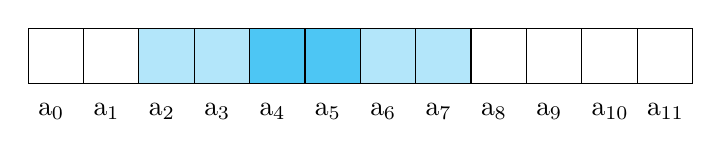
\begin{tikzpicture}
\newcommand{\rectsize}{20}
\filldraw[color=cyan!30] (2*\rectsize pt, 0) rectangle(8*\rectsize pt, \rectsize pt);
\filldraw[color=cyan!70] (4*\rectsize pt, 0) rectangle(6*\rectsize pt, \rectsize pt);
\draw[step=20pt] (0,0) grid(12*\rectsize pt, \rectsize pt);
\foreach \x in {0,...,11} 
  {
    \draw (\x * \rectsize pt, - \rectsize / 2 pt) node[anchor=west]{a\textsubscript{\x}};
  }
\end{tikzpicture}
\end{document}

% !Tex root = checkedc.tex

\chapter{Introduction}
\label{chapter:introduction}

The C programming language \cite{Ritchie1988, ISO2011} allows programmers to use
pointers directly. A pointer is an address of a location in memory. Programs may do
arithmetic on pointers, dereference them to read memory, or assign
through them to modify memory. The ability to use pointers directly
makes C well-suited for low-level system programming that is ``close to
the hardware'' and allows programmers to write efficient programs. C
also unifies pointer types and array types. They can usually be used
interchangeably and array subscripting is a synonym for equivalent
pointer operations.

Pointers and the unification of arrays and pointers are one of the
strengths of the C programming language, allowing programmers to write
concise, efficient programs. At the same time, they are a source of
reliability and security problems in modern software. This is
because pointers and array indices are not bounds checked in C and
related languages such as C++. Bounds checking checks that a pointer or
array index is in bounds before it is used to read or write memory. A
pointer to an array object is in bounds if it points to an element of
the array object. An array index is in bounds if the index is greater
than or equal to zero and less than the size of the array.

Between 2010 and 2015, buffer overflows accounted for between 10-16\% of
publicly reported security vulnerabilities in the U.S. National
Vulnerability Database each year \cite{NIST2015}. The vulnerabilities have affected
software implemented in C and C++ that is widely used, including the
Windows and Linux operating systems, the Internet Explorer, Chrome, and
Safari web browsers, the Apache web server, the OpenSSL security
library, scripting language implementations for Bash, Ruby, and PHP, and
media playback software such as QuickTime.

Because pointers and array indices are not bounds checked in C, a
programming error involving them may corrupt memory locations used by
the program. The memory locations may hold data that is important to the
computations being done by the program or data that is essential to the
control-flow of the program, such as return address locations and
function pointers. Memory corruption can lead to a program producing
incorrect results or, in the hands of a malicious adversary, the
complete malfunctioning of the program and the takeover of a running
process by the adversary.

This technical report describes Checked C, an extension to C that provides
bounds checking for pointers and arrays. There are two obstacles to
adding bounds checking to C. First, it is not clear where to put the
bounds information at runtime. Second, it is not clear how to make the
bounds checking efficient for programs where performance matters. The
solution of changing the representation of all C pointer types and
arrays to carry bounds information is not sufficient in practice. C may
be used at the base of systems where hardware or standards dictate data
layout and data layout cannot be changed. C programs must also
interoperate with existing operating systems and software that require
specific data layouts.

\section{Overview}
Checked C addresses the bounds checking problem for C by:

\begin{itemize}
\item
  Introducing different pointer types to capture the different ways in
  which pointers are used. The unchecked C pointer type \code{*} is kept
  and three new {\it checked} pointer types are added: one for pointers
  that are never used in pointer arithmetic and do not need bounds
  checking (\ptr),  one for \emph{array pointer types} that are involved
  in pointer arithmetic and need bounds checking (\arrayptr), and an
  extension to \arrayptr\ for null-terminated arrays (\ntarrayptr).
\item
  For array pointer types (\arrayptr), in keeping with the low-level
  nature of C,  bounds checking is placed under programmer control.
  This differs from languages like
  Java, where bounds checking is completely automatic. A programmer
  declares \emph{bounds}, where the bounds for an \arrayptr\
  variable are given by non-modifying C expressions. These are a subset
  of C expressions that do not modify variables or memory. They include
  local variables, parameters, constant expressions, casts, and
  operators such as addition, subtraction, and address-of (\code{&})
  operators. Static checking ensures that programs declare and maintain
  bounds information properly. The bounds are used at runtime for
  bounds checking.  A runtime bounds check may be optimized away by a
  compiler if the compiler can prove the check always succeeds.
\item
  Introducing different array types to distinguish between arrays whose
  accesses are bounds-checked and existing C arrays whose accesses are
  not bounds-checked. A programmer places the modifier \keyword{checked}
  before the declaration of the bound(s) of the array: \code{int x
  checked[5][5]} declares a 2-dimensional array for which all
  accesses will be bounds-checked.  Arrays with null terminators
  as their last element can be declared using \keyword{nt\_checked}
  instead of \keyword{checked}.
\item
  For structure types with \arrayptr -typed members, a
  programmer declares \emph{member bounds} for those members. A member
  bounds declares the bounds for a member in terms of members of the
  structure type. Member bounds can be suspended temporarily for
  specific variables and objects. Static checking ensures that updates
  to members maintain the member bounds.
\item
  Introducing bounds-safe interfaces to address the problem of
  interoperation between checked code and unchecked code. A bounds-safe
  interface describes the checked interface to unchecked code by declaring
  bounds for unchecked pointers in function signatures and data structures.
  It describes a boundary that is ``checked'' or ``unchecked''
  depending on what kind of code is using it. The
  interface is trusted in checked code (code that uses only checked pointer types).
  Proper usage is enforced via checking at compile time and runtime. For
  code that uses only unchecked pointer types, the interface is descriptive and
  not enforced by
  language checking. This provides a way to upgrade existing code to
  provide a checked interface without breaking existing users of the code.
\item
  Introducing checked program scopes, where bounds checking is the
  default behavior. In a checked program scope, definitions of variables
  and functions can use checked pointer types and cannot use unchecked pointer
  types. Declarations involving unchecked pointer types must provide
  bounds-safe interfaces. Checked program scopes avoid problems with
  subtle misuse of bounds-safe interfaces.
\item
  Reasoning about the correctness of programs with declared bounds
  sometimes requires reasoning about simple aspects of program behavior.
  To support this, lightweight invariants are added to Checked C. A lightweight
  invariant declares a relation between a variable and a simple
  expression using a relational operator. An example would be the
  statement \code{x < y + 5}. Lightweight invariants can be
  declared at variable declarations, at assignment statements, for
  parameters, and for return values. Checked C is extended with rules for
  checking these lightweight invariants. Just as type checking rules are
  defined by the programming language, so are rules for checking
  lightweight invariants. The checking of the correctness of
  programmer-declared bounds is integrated with the checking of
  invariants.
\item
  For the cases where static checking reaches its limits, a programmer
  can introduce dynamic checks that are runtime errors if they fail.
  Dynamic checks use the syntax \keyword{dynamic\_check} \var{e}, where \var{e} is an
  integer-valued expression. A check is similar to an assert, except
  that it is never removed from the program (unless a compiler proves
  it is redundant). It cannot be removed because the integrity of the
  program depends upon it.
\end{itemize}

For an existing C program to be correct, there has to be an
understanding on the part of the programmer as to why pointers and array
indices stay in range. The goals of the design are to let the programmer
write this knowledge down, to formalize existing practices, such as
array pointer parameters being paired with length parameters, and to
check this information.

To simplify bounds and reasoning about bounds for
\arrayptr\ types, pointer arithmetic overflow for \arrayptr\
types is considered a runtime error. Pointer arithmetic involving a null
pointer for \arrayptr\ types is also a runtime error.

Efficiency is addressed by extending the static checking so that it can
guarantee that specific bounds checks will always succeed at runtime for
\arrayptr\ . The static checking
supports the scenario of simple control-flow enclosing the bounds check
guaranteeing that the bounds check will succeed. For example, a for-loop
may iterate only over values within the declared bounds of an
\arrayptr\ variable.

A problem with incorporating static checking into a programming language
is that static checking needs to be something that compilers can do
quickly and deterministically. Static checking can become very expensive
to do, depending on the language of invariants and the inference that
compilers are expected to do. For example, Presburger arithmetic is
integer arithmetic restricted only to addition and less than or equal
operations. It is NP-complete to determine whether a formula in the
first-order logic for quantifier-free Presburger arithmetic is
always true. Even statically checking properties of
simple fragments of real programs can be computationally intractable.

This problem is addressed in two ways. First, the language rules that are
used to check the validity of bounds are limited intentionally.  The rules can
check the validity of bounds that are needed in practice.  However, there are
bounds that are true that cannot be proved using the rules.  In the terminology
of program logics, the rules are incomplete.  As an example, the
rules about distributivity limit the size of
expressions that they produce.   In practice, this means that
simple disjunctive bounds can be checked, but complex disjunctive bounds cannot be checked.

Second, the inference that compilers do for checking program invariants is
limited.  Compilers act as \emph{checkers} for invariants. They check that
declared invariants follow from other declared invariants, the
program control-flow, intervening assignments, and simple axioms about
invariants, such as transitivity of relational operators. Compilers
do not try to devise invariants or prove the correctness of
invariants; they apply simple local reasoning to check them. The
programmer has to call out the relevant facts. If a programmer declares
an invariant \code{x == y} but neglects to declare the invariant
\code{y == z}, a checker may not be able to reason several
statements later that \code{x == z}, even though it may be true at
that point in the program. This is taking advantage of the fact that
checking a proof is usually much easier than creating the proof.

Establishing the bounds-safety of pointer operations is just the first step in
establishing type safety for C programs. There are other ways which C
programs may fail. C programs may incorrectly deallocate memory that is
still in use, do incorrect type-unsafe pointer casts, or have concurrency
races that tear data structures. Addressing these problems is beyond the
scope of this technical report. For now, it is assumed that programs are
correct in these other aspects.

This design is being done in an iterative fashion.  To validate the
design, we mocked up modifying a subset of the OpenSSL
code base \cite{OpenSSL2015} to be bounds-safe.
We created C++ templates for the new pointer types and modified OpenSSL to
compile as valid C++ code.
We hand-edited about 11,000 lines of the code to use checked pointer
types with full bounds annotations.  We used macros to encapsulate
the bounds annotations so that they could be elided from the code
and OpenSSL compiled and tested using the new types.  We also modified the
generic stack type in OpenSSL to use the \code{ptr} type, which required
cross-cutting changes across the code base (in all, about 160 files were changed)
as well dealing with complicated macros.

We learned the following from this
experience.   First, it was important to have a compact, succinct syntax
for declaring bounds.
Second, in most cases, declaring bounds at declarations was sufficient for
tracking the bounds of variables.  Large blocks of code
remained unchanged, which matches the observations of the
Cyclone project \cite{Jim2002}, an earlier research
effort to create a type-safe version of C.
Third, the expressions allowed in declaring
bounds needed to be rich.  Fourth, pointer casts were used
fairly extensively, but often times it was obvious that the casts were
correct with respect to bounds.  The existing bounds could be modified
easily to be appropriate for the new referent type of the pointer.
Fifth, it was clear that there needed
to be a graceful way of interoperating with existing libraries that could
not be changed.   Finally, signed integer overflow was a pervasive
possibility, which raised questions about the meaning of bounds
declarations that used signed integers.

We revised the design to
address these issues.  In particular, we paid close attention to
tracking bounds through pointer casts.  We also made sure that the
constraints on signed integer expressions used in bounds expressions
were understood and could be written down in the language of
simple invariants.

\section{Principles for extensions}
\label{chapter:principles}

Here are the principles that are followed to extend C to support bounds checking:

\begin{enumerate}
\item
  Preserve the efficiency and control of C. C is designed to be
  low-level and work with the same types that computer processors work
  with. This allows programmers to
  control what programs do precisely at the
  machine level. This efficiency and control are reasons why C is valued as a
  system programming language. Extensions will be ``pay-as-you-go'' and
  continue to provide precise control to programmers at the machine
  level. Hidden costs will be avoided.
\item
  Be Minimal. This means adding the minimal set of extensions needed to
  accomplish the goals. It is easier to learn extensions if there are as
  few of them as possible. It also stays true to the design goals
  of C.
\item
  Aim for clarity and succinctness. Clarity means that code is easy to
  understand and extensions are straightforward to understand.
  Succinctness means the programmers have less to read or type.
  Programmers value clarity and succinctness because it makes them more
  productive.  Sometimes clarity and succinctness are in
  tension and sometimes they are not. When they are in conflict, clarity
  will be prioritized above succinctness, primarily because source code
  is usually read many more times than it is written.
\item
  Enable incremental use. Real systems are large and complicated, with
  hundreds of thousands and millions of lines of code. The teams that
  work on those systems will adopt checked pointer operations over time,
  not all at once, so incremental use of checked pointer operations will be
  supported. Teams will prefer incremental conversion paths because of
  practical matters such as reducing risk, fixing existing bugs
  identified by introducing bounds checking, maintaining system
  stability, and understanding performance effects. Even though
  incremental use will be supported, it is not the end goal. We believe
  that benefits of using checked pointer operations will be modest until
  almost an entire system is converted. At that point, we expect a
  qualitative increase in system reliability and programmer
  productivity.
\end{enumerate}

Two specific design principles are adopted based on these principles:

\begin{enumerate}
\item
  Do not change the meaning of existing C code. Methods that do not use
  extensions will continue to compile, link, and run ``as is''. If the
  meaning of existing C code is changed, it will violate the principles
  of clarity and enabling incremental adoption.
\item
  Adopt existing notations from C++ when they meet our needs, instead of
  inventing new notations. Many systems are hybrid C/C++ systems, so
  this approach fits with the principle of clarity. It also enables
  incremental adoption. One of the design goals of C++ has been that C
  is a subset of C++.  It is a design goal to allow Checked C extensions
  to be amenable to being added to C++ too, so that Checked C is a subset
  of a Checked C++.
\end{enumerate}

\section{Notation}
This specification includes many code examples.   Code will be shown in a teletype font (like \texttt{\small this}).
Operators and symbolic characters will be shown in black (like \lstinline|->|).    Keywords will be shown in blue and program
variables will be shown in light blue (like \lstinline|for (int i = 0; i<10; i++)|).   At times, we will
define properties or make mathematical statements that range over sets of values or program
elements, such as mathematical integers, variables, or expressions.   We will use meta-variables in {\it italics} that
range over these values or program elements.  We might say something like
``for all expressions \var{e\textsubscript{1}} and \var{e\textsubscript{2}}.''   These meta-variables
 differ from program variables, which are elements of specific C programs.

\section{Organization of this document}

Chapter~\ref{chapter:core-extensions} describes
the new pointer types and the new array types, including syntax,
semantics, and error conditions. It also covers other extensions to C
semantics. One extension is the introduction of checked program scopes to
prevent inadvertent use of unchecked types. Another extension is a
refinement of C's notion of undefined behavior. We wish to maintain
bounds safety even in the face of integer overflow, which is a
widespread possibility in C programs. This requires a more nuanced
requirement on the result of overflow than ``the result is undefined.''

Chapter~\ref{chapter:tracking-bounds} describes how programmers declare the bounds for
\arrayptr\ variables and structure members. It also describes the meaning of bounds declarations.
Bounds can be declared at variable declarations. They can also be
declared for local variables at expression statements. If the only
bounds declaration for a variable is at the declaration of the variable,
the bounds declaration is an invariant bounds declaration that is true 
for the lifetime of the variable. If there are bounds declarations for the
variable at assignments or other declarations, all bounds declarations for the variable are
dataflow-sensitive. Dataflow-sensitive bounds declarations extend via
dataflow to uses of the variable.

Invariant bounds declarations must usually be valid after every
statement and declaration in the scope of a variable. Sometime multiple
statements are needed to update the variables in a bounds
declaration.
To support this, expression statements and
declarations can be be replaced in \emph{bundled} block, in which
case bounds declarationsmust be valid only at the end of the block.
In the bundled block, the variables may be inconsistent with respect to
bounds declarations that use them. 

Member bounds declarations are type-level invariants about members
of structure types. We assume that that concurrency control is
been done correctly for those data structure.  Race conditoin in
updates could make the type-level invariants invalid.

When pointers to structure are used to modify members, Checked C requires
that modifications to members preserve type-level bounds invariants.
This follows the lead of the Deputy system \cite{Condit2007}.

Chapter~\ref{chapter:interoperation} covers interoperation between
checked and unchecked code. It covers conversions between checked and
unchecked pointers, as well as conversions between the new kinds of checked pointers.
It pins down the notion of checked code  and unchecked code. Finally, it covers
bounds-safe interfaces in depth.

Chapter~\ref{chapter:checking-bounds} describes rules that the compiler uses to check the validity
of bounds declarations. It covers inferring bounds for expressions.
Because expression may have assignments embedded within them, it also
covers inferring effects of an expression on the bounds of variables.
This inferred information is then used to validate that declarations and
statements correctly declare bounds and maintain the bounds information.

Chapter~\ref{chapter:simple-invariants}
extends the checking of bounds to incorporate simple
reasoning about bounds and program behavior. It includes a set of rules
for deducing facts that are true about a program at a specific point in
the program (for example, given an assignment \code{x = y;} the fact
that x == y is true after the assignment). Facts can also be deduced
from program control-flow. There are additional rules for reasoning
about whether one fact is true given a set of other facts (for example,
given x == y and the statement \code{z = y;} z == x is true after that
statement). These rules and facts can be used to deduce the correctness
of bounds declarations that differ from those inferred directly by the
checking described in Chapters~\ref{chapter:checking-bounds}. For example,
a programmer may wish to narrow the memory that is accessible via an
\arrayptr\ variable by declaring bounds that are a subrange of
the bounds inferred by the checking. A programmer may wish to update the
bounds for an \arrayptr\ variable after an assignment \code{x = y}, substituting
\code{x} for \code{y}.

The same static checking that is used for bounds can be used to reason
about the ranges of variables at specific points in a program. From
there, it is a short step to deducing at compile-time that bounds are
always satisfied at a particular memory access in a program. For
example, a fact can be that the range of an integer variable \code{i}
is always between 0 and 10. This can be used to deduce that an array
access in a crucial inner loop is always in bounds.

Chapter\ref{chapter:roadmap} describes future planned features for Checked C.
These feature are currently not implemented in the Checked C compiler.

\omitted{
Chapter~\ref{chapter:eval} evaluates the design by describing our experience modifying
an existing C open-source code base by hand to use the Checked C
extensions. We chose to modify OpenSSL, an important widely-used
open-source code base. The static and dynamic checking is not
implemented in a compiler yet, so we cannot be sure of the correctness
of the modifications or understand the practical benefits of checking.
Still, this gives some idea about the usefulness and applicability of
the design.

Chapter~\ref{chapter:open-issues} summarizes the open problems uncovered by
Chapter~\ref{chapter:eval} or
unaddressed by the design. It also describes next steps for implementing
this in a C compiler.
}

Appendix~\ref{chapter:related-work} describes related work that addresses
the lack of bounds checking in C.  Because of the serious practical consequences
for computer security and software reliability, there has been extensive work
in the area.  We are heavily influenced by the Deputy system \cite{Feng2006,Condit2007}.

Appendix~\ref{chapter:design-alternatives} discusses design alternatives
that were considered and not chosen.  It explains why those alternatives were
not chosen.

\section{Acknowledgements}

This design has benefited from many discussions with Weidong Cui, Gabriel Dos Reis,
Sam Elliott, Chris Hawblitzel, Galen Hunt, Shuvendu Lahiri, and Reuben Olinsky.  The design has
benefited also from feedback from Michael Hicks, Wonsub Kim, Greg
Morrisett, Jonghyun Park, and Andrew Ruef. We thank them for their contributions to
the design.



% !Tex root = checkedc.tex

\chapter{Extensions to existing C concepts}
\label{chapter:core-extensions}

This chapter describes extensions to existing C concepts. 
It covers new kinds of pointer types and array types, their meaning,
and the operations  on them.   It introduces two
new program scopes: \texttt{check} and \texttt{unchecked}
blocks. It covers a generalization of assertions to 
dynamic checks that are never  removed (unless a compiler
proves them redundant) because bounds safety depends upon them. 
Finally, it describes changes to
undefined behavior needed for bounds safety.

\section{New kinds of pointer types}
Three new safe pointer types are added to C. Each pointer type can be
used in place of `*'

\begin{enumerate}
\item
  \ptrT: this points to
  a value of type \textit{T}. Pointer arithmetic is not allowed on these
  kinds of pointers. The expectation is that that many pointers are not
  involved in pointer arithmetic and will be given this type. When
  values of this pointer type are used to read or write memory, they
  must be non-null. The non-nullness is checked at runtime if necessary.
  The name \ptr\ is chosen for these kinds of pointers because these
  are expected to be the most common type of pointer in C code. \ptr\
  is a short succinct name.
\item
  \arrayptrT: this is
  a pointer to an element of an array of type \var{T} values. A
  variable of type \arrayptr\ that is used to access memory
  must have an associated declaration of the valid bounds for the
  variable. When values of this pointer type are used to read or write
  memory, they must be non-null and in bounds. The non-nullness and
  bounds are checked at runtime if necessary. Pointer arithmetic can be
  done on these pointer types. The resulting pointers do not need to be
  in bounds.
\item
  \arrayviewT: this
  is a pointer that dynamically carries its bounds information with it.
  These pointers follow the same rules as
  \arrayptrT .
\end{enumerate}

Unsafe C pointer types that use \texttt{*} and are unchecked in their
ranges continue to exist. Pointer arithmetic is not forbidden on unsafe
pointer types because it would break existing C code. C compilers will
have an error or warning mode that flags unexpected uses of `*'.

The same syntax as C++ template instantiations is used for building
instances of these types because this syntax is well-known and
understood. The parameter to these type constructors must be a type.

\section{New kinds of array types}

A new safe array type is added to C. Just as there are safe pointer
types, there are safe array types. They are declared by placing the
modifier \keyword{checked} before the declaration of the bound of the
array\footnote{We can just as easily adopt the syntax that the checked
annotation is postfix and propagates from the inner most array to the
 outermost array. We have chosen the prefix syntax because the notation
 can be read easily from left to right ``this is a checked array of
 10x10 elements''.}:
\begin{verbatim}
int a checked[10];
\end{verbatim}

All array references to checked array types are bounds checked. C has
the rule that an ``array of \var{T}'' is converted implicitly to a
``pointer to \var{T}'' in a number of situations. This rule is extended
to convert a ``checked array of \var{T}'' to an ``\arrayptr\ 
to \var{T}''.

In C, array types may be complete or incomplete. A complete array type
specifies the bound of each dimension of the array using constant
expressions. An incomplete array type does not specify the bound of the
first dimension of the array. Examples of complete array types are
\texttt{int[10]} and \texttt{int[10][10]}. Examples of
incomplete array types are \texttt{int[]} and \texttt{int[][10]}.

If a checked array type is incomplete, there must be an associated
declaration of the valid bounds for the first dimension of the array.
For a complete array type, the bounds declared by the type are used to
bounds check array references. For example, given a declaration
\texttt{int a[10]} and a use \texttt{a[i]}, the bounds check is
that \texttt{i >= 0} and \texttt{i < 10}.

Array references to multi-dimensional arrays must be uniformly bounds
checked or not bounds checked. If any dimension is bounds checked, all
dimensions must be checked. A programmer can simply declare the
\emph{``checked''}-ness for the outer dimension. It will be propagated
to the inner dimensions:

\begin{verbatim}
int b checked[10][10];
\end{verbatim}

More specifically, in C, multidimensional arrays are arrays of arrays,
where the nested array types have known dimensions at compile-time. A
2-dimensional array is an array of array of T, a 3-dimensional array is
an array of array of array of T. The checked-ness is propagated from the
outer array to the nested array types.

The propagation works as follows. In C, a declaration of a variable has
the form T D, where T is a type and D is a declarator. The declarator
can be as simple as an identifier \texttt{x}:
\begin{verbatim}
int x;
\end{verbatim}

It can be a more complex form that declares an identifier and modifies T
to produce a new type for the identifier. An example is \texttt{x[5]}:

\begin{verbatim}
int x[5];
\end{verbatim}

Given a C declaration \var{T} \var{D}, if \var{D} is an array
declarator, it will have the form
\texttt{\var{D1}[\var{constant-expression\textsubscript{opt}}]},
where \var{D1} is another declarator. The type of the identifier in the
declaration \var{T D1} will be determined first. The type can be some
constructed type of the form \var{type-modifier} of \var{T}, where
\var{type-modifier} is a sequence of array, checked array, or pointer
type modifiers. If the first element in the \var{type-modifier}
sequence is an array or pointer, the type of the identifier will be
\var{type-modifier} array of T. If the first element in the
\var{type-modifier} sequence is checked array, the type of the
identifier will be \var{type-modifier} checked array of T.

For example, in parsing the declaration of \texttt{b} above, \var{D1}
will be \texttt{int b checked[10]}. The type of \texttt{b} in
\var{D1} is ``checked array of int''. The type of \texttt{b} in
\texttt{int b checked[10][10]} will be ``checked array of
checked array of int''.

\subsection{An example}

It is easy to convert a function that operates only on complete array
types to one where array accesses are bounds checked: just add the
checked keyword to the declarations of the variables with complete array
types. Consider a method that adds 2x2 integer arrays \texttt{a} and
\texttt{b} so that \texttt{a} = \texttt{a} + \texttt{b}:

\begin{verbatim}
void add(int a checked[2][2], int b checked[2][2])
{
    for (int i = 0; i < 2; i++) {
        for (int j = 0; j < 2; j++) {
            a[i][j] += b[i][j];
        }
    }
}
\end{verbatim}

\section{Operations involving pointer types}

The following operations involving pointer-typed values are allowed:

\begin{itemize}
\item
  Indirection: the \texttt{*} operator can be applied to a value of type
  \var{T} \texttt{*},
  \ptrT,
  \arrayptrT, or
  \arrayviewT. It
  produces a value of type \var{T}.
\item
  Array reference: the \texttt{[]} operator can be applied to a
  value of type \var{T} \texttt{*}, \arrayptrT, or \arrayviewT. It
  cannot be applied to a value of type \ptrT.
  \texttt{\var{e1}[\var{e2}]} is equivalent to
  \texttt{*(\var{e1} + \var{e2})}
\item
  Assignment: two pointers of the same type can be assigned.
\item
  Adding or subtracting a pointer type and an integer. This is allowed
  for \var{T} \texttt{*}, \arrayptrT, and \arrayviewT types.
\item
  Pointers to objects of the same type can be compared for equality or
  inequality. The pointers do not have to be the same kind of pointer.
  To support reasoning about program behavior, the result of comparing
  pointers to different objects must be defined.
\item
  Pointers to objects of the same type can be compared relationally,
  except for \ptr\ types. Relational comparisons are the
  \verb|<|, \verb|<=|, \verb|>|, \verb|>=| operators. The pointers do not have to be
  the same kind of pointer. Given a type \var{T}, a \var{T}
  \texttt{*}, \arrayptrT\ or   \arrayviewT, can be compared to a \var{T} \texttt{*},
  \arrayptrT , or \arrayviewT. For example, an \arrayviewT can be compared with an
  \arrayptrT . To support bounds checking and reasoning about program behavior, the
  result of comparing pointers to different objects must be defined.
  Section~\ref{section:changes-to-undefined-behavior} describes this requirement in detail.
\item
  Pointers to objects of the same type can be subtracted, except for
  \ptr\ types. The pointers do not have to be the same kind of
  pointer. The result of subtracting pointers to different objects of
  the same type must be defined. Section~\ref{section:changes-to-undefined-behavior}
  describes this requirement in detail.
\end{itemize}

A value of one pointer type may be converted to a value of another
pointer type. For casts to or from safe pointer types where
bounds-safety can be checked at compile-time, a cast operator can be
used. If bounds safety cannot be checked at compile-time, bounds cast
operators must be used. There are two kinds of bounds cast operators:
\keyword{dynamic\_bounds\_cast}, which does runtime checks of any
conditions required to enforce bounds safety and
\texttt{unchecked\_bounds\_cast}, which does no runtime checking and
trusts the programmer. The rules for pointer casting and the bounds cast
operators are described in Section~\ref{section:pointer-casting}.

\subsection{Rules for the address-of operator}

If an address-of operator (\texttt{\&}) applied to an lvalue expression
of type \var{T}, the following rules apply:

\begin{itemize}
\item
  If the operator occurs in a checked block, the address-of operator
  produces a value of type
  \ptrT
\item
  Otherwise, the address-of operator produces a value of type \var{T}
  \texttt{*}.
\end{itemize}

If the \& operator is applied to an lvalue expression that is a
dereference of a pointer or an array that has bounds checking, the
bounds check will be done when the address is taken. This guarantees
that it is valid to dereference the pointer that results from the
address-of operator. For example, in the following code, bounds checks
will be done at \texttt{\&a[i]} and \texttt{\&b[0]}.

\begin{verbatim}
int a checked[10];
array_ptr<int> b;
int i;
...
ptr<int> y = &a[i];
ptr<int> z = &b[0];
\end{verbatim}

\subsection{Rules for conversion of checked array types to pointer types}

If the type of an expression or a subexpression is ``checked array of
\var{T}'', the type of the expression is altered to be
\arrayptrT.

Following existing C language rules, this alteration does not happen if
the expression is an operand of an address-of operator, \texttt{++},
\texttt{--}, \texttt{sizeof}, or the left operand of an assignment
operator or the `\texttt{.}' operator. The prohibition against this
conversion occurring for operands of the address-of operator gives the
results of the operator a more precise type. For sizeof, it also results
in a more precise answer. The prohibitions against it for ++, and --
operands and the left operand of an assignment operato keeps array
variables from being modifiable.

\subsection{\texttt{Array\_view<}\textit{T}\texttt{>} specific operations}

An \arrayviewT
pointer carries three values with it: the memory location that will be
accessed by dereferencing the
\arrayviewT, a lower
bound on the memory that can be accessed via the current pointer value,
and an upper bound on accessible memory. Those values can be accessed
using the \texttt{.} operator combined with the special field names
\texttt{current}, \texttt{lower\_bound}, and \texttt{upper\_bound}. The
resulting values have the type
\arrayptrT. The
special field names can only be read and cannot be modified by
assignments.

\begin{verbatim}
array_view<int> p = ...
array_ptr<int> low = p.lower_bound;
array_ptr<int> high = p.upper_bound;
array_ptr<int> current = p.current;
\end{verbatim}

An \arrayviewT value
is created by casting a value of another pointer type to the
\arrayviewT type. A
value of another pointer type may be converted to an
\arrayviewT in
situations where an
\arrayviewT value is
expected, the referent type of the other pointer type is \var{T}, and
the bounds of the value can be determined automatically.

For example, a variable of array type can be converted automatically to
an \arrayview\ . First, the array type will be converted to a
pointer type of either \var{T} \texttt{*} or
\arrayptrT , depending
on whether the array type is checked or unchecked. This pointer type
will then be converted to an
\arrayviewT. The
bounds of a variable of array type are easily determined at compile
time, so the pointer type will then be converted to an
\arrayviewT:

\begin{verbatim}
int x[10]
array_view<int> p = x; 
// p.current = x; p.lower_bound = x; p.upper_bound = x + 10;

\end{verbatim}

Similarly, an \arrayptr\ value with declared bounds can be
converted to an \arrayview\ value:

\begin{verbatim}
array_ptr<int> src = ...
array_view<int> p = src;
\end{verbatim}

The full rules for casting to an \arrayview\ type are covered
in Section~\ref{section:pointer-casting}.

\section{Pointer arithmetic error conditions}

For existing unsafe C pointers, the definition of pointer arithmetic is
described in terms of addresses of elements of an array object. The C
Standard \cite{ISO2011} states, that given a pointer p that points to some element i of
an array object, p + j points to the (i+j)th element of that object.
Pointer arithmetic is defined only for pointers to elements of the array
object or one past the last element of the array object.

We take an alternative approach to defining the meaning of pointer
arithmetic and the error conditions for pointer arithmetic. Pointer
arithmetic is allowed to go out-of-bounds and has a well-defined
semantics. Section~\ref{section:new-pointer-types-semantics}
defines the semantics of the new pointer types
directly in terms of byte addresses, instead of with respect to
addresses of elements of an array. Pointer arithmetic that overflows or
involves a null pointer is defined to produce a runtime error.

The new pointer types allow pointer arithmetic that produces
out-of-bounds values. The C definition leaves pointer arithmetic that
produces out-of-bounds values undefined because it is not clear what the
meaning of should be when the pointers are dereferenced. The new pointer
types prevent out-of-bounds pointers from being dereferenced, and solve
this problem another way. In addition, in practice C implementations
often allow pointer arithmetic to produce out-of-bounds values and C
programs end up relying on this implementation-specific behavior. There
is no reason to cause existing code that computes out-of-bounds pointers
but does not dereference them to break when it is converted to use the
new pointer types.

When pointer arithmetic overflows or involves a null pointer, the
resulting value of the expression cannot be used and program execution
stops. If a system provides for error handling, an error handling
mechanism may be invoked to redirect program execution to a new point of
execution that does not use the value of the expression.

Defining pointer arithmetic this way simplifies reasoning about the new
pointer types. Expected Identities such as \texttt{p + 1 > p} now hold
because, if \texttt{p + 1} overflows, the value cannot be
used. This allows programmers to narrow the bounds for
\arrayptr\ values by incrementing the lower bound or
decrementing the upper bound, even in situations where the bounds are at
the ends of the address space. Later sections describe places where
allowing an undefined value to be used would complicate reasoning about
programs.

If a compiler cannot prove that a new pointer type value is non-null
before a pointer arithmetic operation, it must insert a check.
Similarly, if a compiler cannot prove that a pointer arithmetic
expression for a new pointer type cannot overflow, it must insert a
check. This may slow a typical program down by a slight amount.

\subsection{Semantics of pointer arithmetic for new pointer types}
\label{section:new-pointer-types-semantics}

This section defines the semantics of pointer arithmetic and explains
when overflow occurs in pointer arithmetic. It is assumed that memory is
addressable at the byte level. The order of bits within a byte is not
specified. The order of bytes within built-in types larger than a byte,
such as integers and floating-point numbers, is also not specified.
Pointers shall be treated as addresses of locations of bytes in memory.
The addresses shall be unsigned integers with a defined range of 0 to
\texttt{UINTPTR\_MAX}. The maximum value of a signed integer that can be
added to an address shall be given by \texttt{INTPTR\_MAX} and the
minimum value of a signed integer that can be added to an address shall
be given by \texttt{INTPTR\_MIN}.

For the new
\arrayptrT\ pointer
types, there are distinct operations for addition and subtraction of
pointers by signed and unsigned integers. The operations behave
similarly, but have different overflow conditions for scaling because
the ranges of signed integers and unsigned integers are different.

\begin{itemize}
\item
  First scaling an integer by \sizeof{\var{T}} is
  defined. To scale an integer \var{i}, \var{i} shall be multiplied by
  \sizeof{\var{T}}, producing an integer \var{j}. If
  \var{i} is a signed integer, the scaled result shall be treated as a
  signed integer. If \var{i} is an unsigned integer, the scaled result
  shall be treated as an unsigned integer. For a signed integer, the
  minimum and maximum range for j shall be \texttt{INTPTR\_MIN} and
  \texttt{INTPTR\_MAX} For an unsigned integer, the minimum and maximum
  range for j shall be 0 and \texttt{UINTPTR\_MAX}. If \var{j} is
  outside its valid range, the operation doing the scaling operation
  shall produce a runtime error.
\item
  \var{p} \texttt{+} \var{i}, where p is an
  \arrayptrT\ pointer
  and \var{i} is an integer. The integer \var{i} shall be scaled by
  \sizeof{\var{T}}, producing an integer \var{j}. The
  pointer p will be interpreted as an unsigned integer. The mathematical
  value \var{p} + \var{j} shall be the result of the operation. If
  \var{p} + \var{j} is out of range for a pointer, the operation shall
  produce a runtime error.
\item
  \var{i} \texttt{+} \var{p}, where \var{p} is an
  \arrayptrT\ pointer
  and \var{i} is an integer, shall be defined as \var{p} \texttt{+}
  \var{i}.
\item
  \var{p} \texttt{-} \var{i}, where \var{p} is an
  \arrayptrT\ pointer
  and \var{i} is an integer. The integer \var{i} shall be scaled by
  \sizeof{\var{T}}, producing an integer \var{j}. The
  pointer \var{p} will be interpreted as an unsigned integer. The
  mathematical value \var{p} - \var{j} shall be the result of the
  operation. If \var{p -} \var{j} is out of range for a pointer, the
  operation shall produce a runtime error.
\item
  \var{p} \texttt{-} \var{q}, where \var{p} and \var{q} are
  \arrayptrT
  pointers. The two pointers will be interpreted as unsigned integers
  and the mathematical value \var{p} - \var{q} shall be computed,
  producing an integer \var{j}. If \var{j} is out of range for signed
  integer that can be added to an address, the operation shall produce a
  runtime error. If \var{j} is a multiple of
  \sizeof{\var{T}}, the result shall be
  \var{j}/\sizeof{\var{T}}. If \var{j} is not a
  multiple of \sizeof{\var{T}}, then the value shall
  be determined as follows:

  \begin{itemize}
  \item
    If \var{j} is non-negative,
    \var{j}/\sizeof{\var{T}} shall round toward 0.
  \item
    If \var{j} is negative, it shall be implementation-defined whether
    \var{j}/\sizeof{\var{T}} rounds toward 0 or away
    from 0.
  \end{itemize}
\end{itemize}

An important implication of these definitions is that they put a maximum
limit on the number of elements in an array of type \var{T}. It is
\texttt{UINTPTR\_MAX}/\sizeof{\var{T}}. They also put
maximum limits on the number of elements that can be accessed in an
array by a signed integer or an unsigned integer. That leads to limits
on the size of arrays that can be described by some bounds. A signed
integer that must be non-negative can describe an array of
\texttt{INTPTR\_MAX/\sizeof{\var{T}}} elements.

\subsection{Expressing pointer arithmetic as integer arithmetic}
\label{section:pointers-as-integers}

During static checking, pointer arithmetic operations will be converted
to use integer arithmetic. This is necessary in C because at times
programmers do explicit size computations that follow the same rules as
pointer arithmetic.

To support this expansion, integer arithmetic operators are extended
with the operators \texttt{+\textsubscript{ovf}},
\texttt{-\textsubscript{ovf}} , and\texttt{*\textsubscript{ovf}}. The
operators interpet pointers as unsigned integers in some range 0 to
\texttt{UINTPTR\_MAX}. An operator produces a runtime error if the value
of its result cannot be represented by the result type:

\begin{itemize}
\item
  \texttt{+\textsubscript{ovf}} takes an unsigned integer i and an
  integer j and produces an unsigned integer in the range 0 to
  \texttt{UINTPTR\_MAX}. Its result is the mathemetical value i + j.
\item
  For subtraction, there are two forms:

  \begin{itemize}
  \item
    \texttt{-\textsubscript{ovf}} takes an unsigned integer i and an
    integer j as an argument and computes i - j, producing an unsigned
    integer in the range 0 to \texttt{UINTPTR\_MAX}. Its result is the
    mathematical value i - j.
  \item
    \texttt{-\textsubscript{ovf\_diff }}takes two unsigned integers i
    and j and computes i - j, producing a signed integer of type
    \texttt{ptrdiff\_t}. Its result is the mathemetical value i - j.
  \end{itemize}
\item
  \texttt{*\textsubscript{ovf }}takes two integers i and j (both either
  signed or unsigned) as arguments. It produces an integer whose type is
  the same as the input argument types. Its result is the mathematical
  value i * j.
\end{itemize}

Given an expression \texttt{e1} with a pointer type and an expression
\texttt{e2} with an integer type, the expansion of \texttt{e1 + e2} from
pointer arithmetic to integer arithmetic depends on the type of
\texttt{e2}. The number of bytes to added must be the same kind of
signed or unsigned integer as \texttt{e2}.

\begin{itemize}
\item
  If \texttt{e2} is an unsigned integer, \texttt{e1 + e2} expands to
  \texttt{e1 +\textsubscript{ovf} \sizeof{\var{T}} *\textsubscript{ovf} e2}
\item
  If \texttt{e2} is a signed integer, the expansion of \texttt{e1 + e2}
  must cast \sizeof{\var{T}} to a signed integer. We introduce a
  signed integer type \texttt{signed\_size\_t} that is large enough for
  this cast. \texttt{e1 + e2} expands to \texttt{e1 +\textsubscript{ovf}
  ((signed\_size\_t) \sizeof{\var{T}} *\textsubscript{ovf} e2}. This cast is
  necessary because in C, multiplying a signed integer by an unsigned
  integer implicitly converts the signed integer to be an unsigned
  integer.
\end{itemize}

\subsection{Runtime performance implications}

There will be concerns about the effect of overflow checks on the speed
of pointer arithmetic using the new pointer types. These concerns are an
empirical question to be settled after implementing and using the new
pointer types. It is unclear what the actual cost will be. First, there
will be sometimes be additional conditions on expressions used in
pointer arithmetic that prevent overflow from occurring. Second,
compiler optimizations often can remove the checks. Third, programmers
can use lightweight invariants to show statically that checks are not
necessary.

In our experience working on an operating system written in managed code
that required these checks, the slowdown was a few percent, even when
\emph{all} arithmetic instructions were checked for overflow too. The
cost of checks was low because it is often the case that checks are
redundant or can be combined into adjacent machine instructions. For
example, in the code \texttt{t = *p; p += 1;} the first dereference of
\texttt{p} implies that \texttt{p} is non-null before the increment.
Otherwise, in a typical C environment, the program would fault at
\texttt{*p}. In the code \verb|if (p < hi) { p += 1; }|
the check \texttt{p < hi} implies that the increment cannot
overflow. The checks are also inexpensive on superscalar processors:
they can be placed so that they are statically predicted by the
processor to never fail.

\section{Relative alignment of \arrayptr\ and \arrayview\ values}
\label{section:relative-alignment}

\arrayptrT\ and \arrayviewT\ pointers provide safe
pointer arithmetic on arrays. The bounds for these pointers usually
describe a range of memory that is exactly the size of some array of \var{T}.
The pointers point to an element of the array. In other words, the lower
bound, the upper bound, and pointer are  relatively aligned to the type
\var{T}. Given a lower bound \var{lb}, an upper bound \var{ub}, and a
pointer \var{p}, there should exist some integer \var{count} such that
\var{ub} = \var{lb} + \var{count}. In addition, there is either some
integer \var{index} such that \var{p} = \var{lb} + \var{index},
where addition is C pointer arithmetic, or \var{p} is null.

The type to which a pointer and its bounds are relatively aligned is
called the relative alignment type. By default, the relative alignment
type for a pointer and its bounds is the referent type. However, the
relative alignment type can be overridden by specifying it explicitly as
part of the bounds.  This is described in 
Section~\ref{section:representing-relative-alignment}.
This can be used for bounds for the results of pointers casts and 
for  \arrayptrvoid\ and \arrayviewvoid\ pointers. The type
\texttt{void} has no defined size, so the default relative alignment is
undefined for \texttt{void}.

We considered removing the entire concept of relative alignment from the
design to simplify the design.  We decided against that it because it 
increases cost of bounds checking throughout the program.  
Section~\ref{section:design-alternatives:always-unaligned} explains
this choice in more detail.

\section{Program scopes for safe pointer types}

To improve program reliability and to simplify understanding programs,
it is desirable to limit code to using only safe pointers. To support
this, we introduce checked program scopes. The \keyword{checked} keyword
can be attached to blocks and function definitions. In checked program
scopes, definitions can use only safe pointer types and checked array
types; they cannot use unsafe pointer types and unsafe arrays. On the
other hand, declarations can use unsafe pointer types and unsafe arrays,
provided that the declarations provide a bounds-safe interface.

A new pragma directive \texttt{BOUNDS\_CHECKED} is introduced to control whether
the top-level scope is a checked scope:
\begin{alltt}
#pragma BOUNDS_CHECKED \textit{on-off-switch}
\end{alltt}

Where \texttt{\textit{on-off-switch}} is one of \verb|ON OFF DEFAULT|

By default, function definitions are not checked. A block inherits the
checking properties of its parent. This preserves the meaning of
existing C code.

A checked block is introduced by placing  \keyword{checked} before a
compound block:
\begin{verbatim}
checked 
{
    int a = 5;
    ptr<int> pa = &a;

    int b checked[5][5];
    for (int i = 0; i < 5; i++) {
        for (int j = 0; j < 5; j++) {
            // all references are bounds checked
            b[i][j] = -1;
        }
    }
}
\end{verbatim}

It is rarer for a programmer to need to introduce an unchecked scope. It
is usually needed to allow the use of unsafe pointers within a checked
block. The \keyword{unchecked} keyword can be used in all the places where the
checked keyword can be used. This example shows the use of an unchecked
block:

\begin{verbatim}
checked 
{
    int a = 5;
    unchecked 
    {
        int *upa = &a;	
        int b[5][5];
        for (int i = 0; i < 5; i++) {
            for (int j = 0; j < 5; j++) {
                // not bounds checked
                b[i][j] = -1;
            }
        }     
    }
 ...
}
\end{verbatim}

In a checked function definition, the body of the function is a 
checked  block. A checked function definition is declared by placing the
\keyword{checked} before the definition. Here are examples of checked and
unchecked function definitions:

\begin{verbatim}
// checked at the function level: no unsafe pointers can appear in argument
// types, the return type, or the body of the function.
checked int f(ptr<int> p) 
{
    int a = 5;
    ptr<int> pa = &a;
    ...
}

// unchecked at the function level: Safe and unsafe pointer types can occur 
// in argument types, the return type, or the body of the function
unchecked int f(int *p, ptr<int> r)
{
    int a = 5;
    int *pa = &a;
    ...
}

// f is unchecked by default
int f(int *p, ptr<int> r)
{
    int a = 5;
    int *pa = &a;
    ...
}
\end{verbatim}

When a function call occurs in a checked block, the function being
called does not have to be declared as checked. The notion of whether a
scope is checked or not checked is lexical and the function definition
is a separate lexical scope.

As we add different notions of checking to C programs, we will use the
checked and unchecked keywords for all the different notions of
checking. We may introduce additional keywords to control specific kinds
of checking.

\section{Programmer-inserted dynamic checks}

A bounds check generates a runtime error if it fails. The ability to
generate a runtime error is not limited to the C implementation. A
programmer can check a Boolean condition and generate a runtime error
using the expression \texttt{dynamic\_check(}\var{e1}\texttt{)}, where
\var{e1} is an integral valued expression. At runtime, \var{e1} is
evaluated. If the result is \texttt{0} (false), a runtime error occurs.
If the result is non-zero (true), no runtime error occurs. Just as with
a bounds check, if a runtime error occurs and a C implementation
provides an error-handling facility, the error-handling facility may be
invoked.

The \texttt{dynamic\_check} expression is similar to an assertion, but
unlike an assertion, it is expected to be used in production or release
versions of software. The \texttt{dynamic\_check} expression is useful
for these reasons:

\begin{itemize}
\item
  It provides an escape hatch for limits of static checking. If a
  programmer knows a condition is true at runtime, yet the static
  checking cannot prove the fact, the programmer can use
  \texttt{dynamic\_check} to show that the condition is true.
\item
  It maintains programmer control: programmers can use unsafe ponters
  and \texttt{dynamic\_check} to write the same code that the compiler
  would generate for safe pointers.
\item
  It gives programmers more control over bounds checks. A programmer can
  place a pre-condition before a loop that ensures that the loop is free
  from dynamic bounds checks, without having to restructure the
  control-flow of the program.
\end{itemize}

The following example illustrates why having an escape hatch from static
checking is useful. Suppose a decoder from a compressed representation
to an uncompressed representation is being converted to use safe
pointers. This example is based on code patterns seen in the Abstract
Syntax Notation (ASN1) parsing code of OpenSSL \cite{OpenSSL2015}.

\begin{verbatim}
void decode(char *output_buffer, char *input_buffer, size_t input_len)
{
    char *src = input_buffer;
    char *src_bound = src + input_len;
    char *dst = out_buffer;

    while (src < bound) {
        switch (*current++) {
            case UNCOMPRESSED_BYTES: { 
                // just copy bytes; compression wasn't useful here.
                size_t len = src[0] + src[1]*256;
                src += 2;
                memcpy(dst, src, len);
                src += len;
                dst += len;
                break;
            }
            case COMPRESSED_INT64: {
                ...
                break;
            }
        ...
    }
}
\end{verbatim}

The caller knows that the destination buffer will be large enough and
that the contents of the source buffer are well-formed. However, these
invariants cannot be expressed using lightweight invariants. These are
complicated high-level invariants that require the use of techniques for
proving functional correctness.

To use safe pointers, the size of the destination buffer must be passed
in and there must be a check before the memcpy that the destination
buffer and source buffer have enough room. We ignore the details of how
the bounds are described for now.

\begin{verbatim}
void decode(array_ptr<char> output_buffer, array_ptr<char> input_buffer, 
            size_t input_len, size_t output_len)
{
    array_ptr<char> src = input_buffer;
    array_ptr<char> src_bound = src + input_len;
    array_ptr<char> dst = out_buffer;
    array_ptr<char> dst_bound = out_buffer + output_len;


    while (src < bound) {
        switch (*current++) {
            case UNCOMPRESSED_BYTES: { 
                size_t len = src[0] + src[1]*256;
                src += 2;
                // need check that dst and src have at least len bytes of
                // space
                memcpy(dst, src, len);
                src += len;
                dst += len;                
                break;
            }
            case COMPRESSED_INT64: {
                ...
                break;
            }
        ...
    }
}
\end{verbatim}

How should that check be written? One approach is to change the
control-flow by inserting if-statements into the program. Something must
be done if the check fails, though. One possibility is to just ignore a
failure. This is bad programming practice because now the program might
fail silently:

\begin{verbatim}
void decode(array_ptr<char> output_buffer, array_ptr<char> input_buffer, 
            size_t input_len, size_t output_len)
{
      ...
            case UNCOMPRESSED_BYTES: { 
                size_t len = src[0] + src[1]*256;
                src += 2;
                // check that dst and src have at least len bytes of
                // space
                if (dst + len >= dst_bound || src + len >= src_bound) {
                    goto failure;
                }
                memcpy(dst, src, len);
                src += len;
                dst += len;                
                break;
            }
   ...
   failure: 
      return;
}
\end{verbatim}

This could be fixed by having \texttt{decode} return a status code
indicating success or failure. That just pushes the problem upward to
the caller and leaves a testing problem. The program should never fail,
so there is no way to test the path.

\begin{verbatim}
int decode(array_ptr<char> output_buffer, array_ptr<char> input_buffer, 
            size_t input_len, size_t output_len)
{
   ...
   failure: 
      return 1;
}
\end{verbatim}

The problems with requiring functions that validate buffer lengths to
return status codes for errors are analyzed by O'Donell and Sebor\cite{ODonell2015}. 
Annex K of the C Standard \cite{ISO2011} introduced a new set of standard library functions to replace
functions that provide no way to validate their arguments. These
functions return status codes to indicate success or failure A classic
example of a function prone to misuse is \texttt{strcpy(char *dst, const
char *src)}. It copies all bytes in \texttt{src} to \texttt{dst} until
it hits a null byte. If \texttt{src} is missing the null byte or
\texttt{dst} is too small, this causes a buffer overrunn. The new
function \texttt{strcpy\_s} takes an additional size parameter for
\texttt{dst} and has the signature \texttt{errno\_t strcpy\_s(char *dst,
size\_t dest\_len, const char *src)}. O'Donell and Sebor explain how
using these functions is awkward, leading to more complicated and less
efficient code.

In contrast, \texttt{dynamic\_check} allows the checking to be localized
and not propagate upward in the call chain. If the programmer is
correct, the check never fails. If the programmer is incorrect, the
check might fail and invoke error-handling code:

\begin{verbatim}
void decode(array_ptr<char> output_buffer, array_ptr<char> input_buffer, 
            size_t input_len, size_t output_len)
{
      ...
            case UNCOMPRESSED_BYTES: { 
                size_t len = src[0] + src[1]*256;
                src += 2;
                dynamic_check(dst + len < dst_bound && src + len < src_bound);
                memcpy(dst, src, len);
                src += len;
                dst += len;                
                break;
            }
   ...
}
\end{verbatim}

One can argue that it is a problem to have a dynamic point of failure
that leads to error-handling code being invoked. This is the same way
systems treat null pointer dereferences, though, which are a possibility
throughout C code. The alternative of having a program with undefined
behavior is worse.

The following example uses \texttt{dynamic\_check} to eliminate bounds
checks in a loop. It is based on experience hand-optimizing C\# and Java
programs. This kind of example is typically found during a performance
tuning phase of program development. In the example, 
the \verb|: count(|\var{exp}\verb|)| notation indicates that \var{exp} is the
length of the buffer.

\begin{verbatim}
void append(array_ptr<char> dst : count(dst_count),
            array_ptr<char> src : count(src_count), 
            size_t dst_count, size_t src_count)
{ 
    for (size_t i = 0; i < src_count; i++) {
        if (src[i] == marker) {
           break;
        }
        dst[i] = src[i];
    }
}
\end{verbatim}

The highlighted expressions are bounds checked:
\begin{verbatim}
void append(array_ptr<char> dst: count(dest_count), 
            array_ptr<char> src : count(src_count), 
            size_t dst_count, size_t src_count)
{ 
    for (size_t i = 0; i < src_count; i++) {
        if (src[i] == marker) {
           break;
        }
        dst[i] = src[i];
    }
}
\end{verbatim}

It is clear that the accesses to \texttt{src} are in-bounds based on
just information from the for-loop, so a compiler will eliminate those
bounds checks. It is not clear that assignments through \texttt{dst} are
always in bounds, so the check there must remain. It can be eliminated
by adding a \texttt{dynamic\_check}:

\begin{verbatim}
void append(array_ptr<char> dst: count(dest_count), 
            array_ptr<char> src : count(src_count), 
            size_t dst_count, size_t src_count)
{ 
    dynamic_check(src_count <= dst_count);
    for (size_t i = 0; i < src_count; i++) {
        if (src[i] == marker) {
            break;
        }
        dst[i] = src[i];
    }
}
\end{verbatim}

The compiler now knows that \texttt{i < src\_count
<= dst\_count}, so it can eliminate the check.

A compiler would not introduce this dynamic\_check because it would
alter the behavior of \texttt{append}. The bounds check on \texttt{dst}
in the original code is done only if a marker is not found in
\texttt{src} and \texttt{src\_count \textgreater{} 0}. A compiler could
try to deduce a precondition for the bounds check failing, but this is
not possible because the precondition depends on the contents of
\texttt{src}. A compiler would have to clone code to maintain the same
behavior. This increases code size, so production compilers do not this
sort of transformation or do it sparingly. Programmer control produces
better results.

\begin{verbatim}
void append(array_ptr<char> dst: count(dest_count), 
            array_ptr<char> src : count(src_count), 
            size_t dst_count, size_t src_count)
{ 
    if (src_count <= dst_count) {
        for (size_t i = 0; i < src_count; i++) {
            if (src[i] == marker) {
                break;
            }
            dst[i] = src[i];  // no bounds check needed
        }   
    else {
        for (size_t i = 0; i < src_count; i++) {
            if (src[i] == marker) {
                break;
            }
            dst[i] = src[i];  // bounds check needed
        }   

    }
}
\end{verbatim}

\section{Changes to undefined behavior}
\label{section:changes-to-undefined-behavior}

C has situations where an expression has undefined behavior or the
meaning of an expression is undefined:

\begin{itemize}
\item
  Unsafe pointer arithmetic only has defined behavior when the resulting
  pointer points to the same object as the original pointer, or one
  element past the object.
\item
  Unsafe pointer comparison only has defined behavior when comparing
  pointers to the same object (where one or both pointers may point one
  element past the same object).
\item
  Unsafe pointer subtraction only has defined behavior when subtracting
  pointers to the same object (where one or both pointers may point one
  element past the object).
\item
  Arithmetic expression behavior is undefined on signed integer overflow
  and integer division by 0.
\item
  Expressions may have nested assignments within them. The evaluation
  order of side-effects in subexpressions is defined only in specific
  circumstances; otherwise it is undefined. This leads to expressions
  with undefined meaning. There can be multiple assignments to the same
  variable that have no defined evaluation order with respect to each
  other or an assignment and a use of a variable that have no defined
  evaluation order.
\item
  Initializers may have nested assignments within them. These can have
  undefined meanings as well for the same reasons as expressions.
\end{itemize}

Undefined behavior is different from unspecified behavior, where one of
a number of choices may be made. Unspecified behavior in C includes:

\begin{itemize}
\item
  The order of evaluation of side-effects in expressions (so long as the
  expression does not have undefined behavior).
\item
  The order of evaluation of side-effects in initializers.
\end{itemize}

C also has implementation-defined behavior, which includes:

\begin{itemize}
\item
  The ranges of values for integer, floating-point, and pointer types.
\item
  Data layout, including the sizes of types, padding, and alignment of
  data.
\item
  Some aspects of pointer conversion.
\end{itemize}

It is difficult to reason about the correctness of programs that have
expressions with undefined behavior. One has to make sure that a program
never arrives at a point where behavior is undefined. In practice, this
would mean proving that signed integer overflow can never occur, for
example. For unspecified behavior, one has to reason about all possible
behaviors, such as all possible orders of evaluation. For
implementation-defined behavior, one has to reason about the
implementation-specific behavior or have reasoning that is independent
of the details.

A careful reading of the rules for unsafe pointer comparison implies
that it is impossible to detect an out-of-bounds unsafe pointer in C,
for example. If an unsafe pointer p is not in the valid range for an
object, the pointer comparison is undefined.

To provide for pointer bounds safety, we require that C implementations
provide defined behaviors for unsafe pointer arithmetic operations and
signed integer overflow:

\begin{itemize}
\item
  Unsafe pointers shall be treated as addresses of locations in memory,
  just as safe pointers are treated as addressses. The addresses shall
  be unsigned integers with a defined range of 0 to
  \texttt{UINTPTR\_MAX}:

  \begin{itemize}
  \item
    Comparison of pointers for all different kinds of pointers shall be
    defined as the corresponding integer comparison.
  \item
    Subtraction \var{p} \texttt{-} \var{r} of two pointers \var{p} and \var{r}
    of type \var{T} where one
    pointer is a safe pointer and the other is an unsafe pointer shall
    be done following the rules for subtraction of safe pointers,
    treating the unsafe pointer as a safe pointer in those rules.
  \end{itemize}
\end{itemize}

\begin{itemize}
\item
  To be able to maintain pointer bounds safety, it is important that
  signed integer overflow produce a defined value. When a signed integer
  expression produces an out-of-range value, either (1) the operation
  must convert that value to an in-range integer value or (2) the
  expression shall produce a runtime error. The conversion must be a
  function of only the input values of the expression.
\item
  Integer division by 0 shall also produce a runtime error or produce a
  defined value.
\end{itemize}

In the case of a runtime error, program execution cannot continue in a
way the uses the value of the expression that produced the error.

For programs with expressions and initializers with undefined meanings,
those programs must be rejected at translation-time. 
Section~\ref{section:avoiding-undefinedness}
describes this in detail.

Of course, there are other ways in which C expressions may have
undefined behavior:

\begin{enumerate}
\item
  By reading or writing memory through an out-of-bounds pointer.
\item
  By storing a value of one type and accessing the value as a different
  type later, when the value is not valid for the different type. A
  program might write bit patterns that do not correspond to valid
  values for a type or write an integer and use it as a pointer later,
  even though the pointer is not within the range of memory for a valid
  object.
\item
  By accessing memory that has been deallocated.
\item
  By using variables or functions with inconsistent declarations across
  different translation units. This can cause the type of a variable or
  a function to be different at the definition and the use. This can be
  addressed with suitable link-time checking.
\end{enumerate}

The aim is to be able to show partial correctness of programs for the
first item (avoiding out-of-bounds pointer accesses). A
partial correctness guarantee has the form ``assuming X holds, then Y is
true''. Informally, one might say ``assuming that memory allocation and
type casts are correct and that unsafe code never reads or write though
out-of-bounds pointers, then safe code never reads or writes through
out-of-bounds pointers.'' These assumptions can be turned into formal
statements about program behavior at runtime. Given those assumptions,
we might then prove that at runtime safe code never reads or writes
through out-of-bounds pointers.

% !Tex root = checkedc.tex

\chapter{Bounds for variables}
\label{chapter:tracking-bounds}

Variable with \arrayptr\ types that are used to access
memory must have bounds declared for them.  The same requirement
holds for variables with incomplete checked array types.

For an \arrayptr\ variable, the bounds will be used to check
memory accesses at runtime involving the pointers stored in the variable
or pointers produced by pointer arithmetic that uses those pointers.
Runtime checks can be omitted if a compiler proves that they are
redundant. In addition, for performance-critical code, checks will be
omitted when programmers demonstrate at compile-time that the checks are
redundant (see Section~\ref{section:avoiding-bounds-checks} for details).

\section{Bounds declarations}
\label{section:bounds-declarations}

Bounds are declared using bounds declarations. Bounds declarations have
the form:

\begin{tabbing}
\var{bounds}\=-\var{decl:} \\
\> \boundsdecl{\var{x}}{\var{bounds-exp}} \\
\\
\var{bounds}\var{-exp:} \\
\> \texttt{count(}\var{non-modifying-exp}\texttt{)} \\
\> \bounds{\var{non-modifying-exp}}{\var{non-modifying-exp}} \\
\> \boundsnone \\
\> \boundsany
\end{tabbing}

where \var{x} is a variable. There are additional forms for handling
casts and void pointers that are described in 
Sections~\ref{section:pointer-cast-results} and \ref{section:pointers-to-void}.

A bounds expression describes the memory that can be accessed using the
value of \var{x}, provided that x is not null. Bounds expressions
include counts, pairs that specify an upper bound and lower bound,
\boundsnone, and \boundsany:

\begin{itemize}
\item
  \boundsdecl{\var{x}}{\boundscount{e1}} describes the number of
  elements that are accessible beginning at \var{x}. Only memory that
  is at or above x and below \var{x} \texttt{+} \var{e1} can be
  accessed through \var{x}, where \var{x} \texttt{+} \var{e1} is
  interpreted using \arrayptr\ pointer arithmetic.
\item
  \boundsdecl{\var{x}}{\bounds{\var{e1}}{\var{e2}}}
  describes the range of memory that can be accessed through \var{x}.
  Only memory that is at or above the location specified by \var{e1}
  and below \var{e2} can be accessed through \var{x}.
\item
  \boundsdecl{\var{x}}{\boundsnone} declares that \var{x} has no bounds.
  It is an error at compile-time to attempt to access memory using a
  variable of type \arrayptr\ with no bounds.
\item
  \boundsdecl{\var{x}}{\boundsany} is a special form that readers can
  ignore for now. It is used for null pointers (0 cast to a pointer
  type) and means that \var{x} can have any bounds. Because null
  pointers cannot be used to access memory, they can have any bounds.
\end{itemize}

Bounds expression use ``non-modifying'' expressions. These are a subset
of C expressions that do not modify variables or memory. They include
local variables, parameters, constant expressions, casts, and operators
such as addition, subtraction, and address-of. 
Section~\ref{section:non-modifying-expressions}  describes
non-modifying expressions in detail.

In a bounds declaration of the form \boundsdecl{\var{x}}{\var{bounds-exp}},
\var{x} can have an \arrayptr\ or a checked array type.
For the form  \boundsdecl{\var{x}}{\boundscount{\var{e1}}},  the type of
\var{x} cannot be \arrayptrvoid\ and the type of \var{e1} must be an integral type.
The usual C integer conversions are applied to \var{e1}.\footnote{If the
type of \var{e1} is a character, a short integer, a bit field, or an enumeration type,
the expression is promoted to an \keyword{int} type if that is large
enough to  hold all values of the type or an \keyword{unsigned int} type otherwise.}
For \boundsdecl{\var{x}}{\bounds{\var{e1}}{\var{e2}}}, \var{e1} and
\var{e2} must be pointers to the same type.  Typically \var{x} is also 
a pointer to that type or an array of that type.  
However, \var{x} can be a pointer to or an array of a different type.
This is useful for describing the results of casts and
bounds for \arrayptrvoid\ pointers.

For any variable with a bounds declaration, the variable must be
non-null when memory is accessed There is no requirement that an
\arrayptr\ variable stay within its bounds. The requirement is
that the \arrayptr\ variable can only be dereferenced if it is
in bounds. This avoids bound checks on pointer arithmetic.

Count expressions have limits on their ranges to prevent signed integer
overflow and unsigned integer wraparound from affecting size
computations. Section~\ref{section:integer-overflow-informal}
explains these limits in detail. The limits
depend on the element type of the \arrayptr\ and the type of the count
expression. For \boundsdecl{\var{x}}{\boundscount{\var{e1}}}, where \var{x}
has type \arrayptrT ,
\var{e1} must be greater than or equal to 0. \var{e1} must be less
than the maximum number of an
\arrayptrT\ elements
that can be indexed by an integer whose type matches that of \var{e1}.
A bounds declaration \boundsdecl{\var{x}}{\boundscount{\var{e1}}} is an
abbreviation for \boundsdecl{\var{x}}{\bounds{\var{x}}{\var{x} \texttt{+} \var{e1}}} with additional conditions that \var{e1}
\texttt{>= 0 \&\& \var{e1} <= (char *)}
\var{ub}\texttt{.} \var{ub} is either
\texttt{UINTPTR\_MAX/\sizeof{\var{T}}} or
\texttt{INTPTR\_MAX/\sizeof{\var{T}}}. 

The conditions may require programmers to add additional checks at memory allocations
to show that \var{e1} is in range. However, the conditions have advantages too.
They provide scaffolding for proving that expressions based on
element counts of \arrayptr\ variables do not overflow or wraparound.

The meaning and correctness of bounds are based on the C semantics for
pointers and pointer arithmetic. At runtime, any non-null pointer in C
has an object associated with it. The association starts when a pointer
is created by a memory allocation operation, address-of expression, or
conversion of an array variable to a pointer-typed expression. It flows
through to pointers that result from pointer arithmetic. At runtime, the
bounds for a pointer must be the bounds of the object associated with
the pointer or a subrange of those bounds. The correctness of declared
bounds information at compile-time is ensured by making allocation sites
and address-of expressions be creators of bounds information and by
propagating bounds with the pointers with which they are associated.
Bounds can be narrowed during propagation, but they cannot be widened.

The meaning of a bounds expression can be defined more precisely. At
runtime, given an expression \var{e} with a bounds expression
\bounds{\var{lb}}{\var{ub}}, let the runtime
values of \var{e}, \var{lb}, and \var{ub} be \var{ev}, \var{lbv},
and \var{ubv}, respectively. The value \var{ev} will be \texttt{0} (null) or
have been derived via a sequence of operations from a pointer to some
object \var{obj} with \bounds{\var{low}}{\var{high}}.
The following statement will be true at runtime:
\var{ev} \texttt{== 0 || (\var{low} <= \var{lbv}\&\& 
\var{ubv} <= \var{high})}. In other words, 
if \var{ev} is null, the bounds
may or may not be valid. If \var{ev} is non-null, the bounds must be
valid. This implies that any access to memory where \var{ev} \texttt{!=
0 \&\&} \var{lbv} \texttt{<=} \var{ev} \texttt{\&\&} \var{ev}
\texttt{<} \var{ubv} will be within the bounds of \var{obj}.

In this chapter, to simplify the description, it is assumed that none of
the \arrayptr\ variables that have bounds declarations have
their addresses taken. It is also assumed that the values of variables
whose addresses are taken are not used in bounds declarations. It is
acceptable to use the address of an address-taken variable in a bounds
declaration. This is provided that the resulting address is not used to
access memory in the bounds declaration (that is, indirectly access the
value of a variable). For example, given the declaration \texttt{int x},
the expression \texttt{\&x} may appear in a bounds expression.  
Chapter~\ref{chapter:pointers-to-data-with-arrayptrs} extends the
design to avoid these restrictions.  It covers pointers to data with 
\arrayptr\ values,  pointers to variables used in bounds, and bounds 
that use pointers.

\section{Using bounds declarations}

Bounds declarations may be added to declarations and statements using
\keyword{where} clauses. They also may be placed inline at a declaration
by following the declarator with \texttt{:} \var{bounds-exp}. In that
case, the bounds expression applies to the variable that is the subject
of the declarator. By making the bounds be part of the program, this
preserves the control and efficiency of C. The bounds declarations will
be checked statically for correctness using rules described in 
Chapter~\ref{chapter:checking-bounds}.

\subsection{Bounds declarations at variable declarations}
\label{section:variable-declarations}

Here are some examples of bounds declarations as part of variable
declarations. The first function sums the integers stored in memory
between \texttt{start} and \texttt{end}, where the integer stored at
\texttt{end} is not included.

\begin{verbatim}
int sum(array_ptr<int> start : bounds(start, end), array_ptr<int> end)
{ 
    int result = 0;
    array_ptr<int> current : bounds(start, end) = start;
    while (current < end) {
       result += *current++; // *current is bounds-checked.  The checking ensures 
                             // that current is within the bounds of (start, end) 
                             // at the memory access.                           
    }
    return result;
}
\end{verbatim}

This can be written using \keyword{where} clauses as well, at the
inconvenience of typing variable names twice in declarations:

\begin{verbatim}
int sum(array_ptr<int> start where start : bounds(start, end), array_ptr<int> end)
{ 
    int result = 0;
    array_ptr<int> current where current : bounds(start, end) = start;
    while (current < end) {
       result += *current++;                          
    }
    return result;
}
\end{verbatim}

This function searches for an integer in an array. If it finds the
integer, it returns the index in the array where the integer occurs.
Otherwise, it returns -1.

\begin{verbatim}
int find(int key, array_ptr<int> a : count(len), int len)
{
    for (int i = 0; i < len; i++) {
         if (a[i] == key) { // a[i] is bounds checked.  The checking
                            // ensures that i is between 0 and len.
             return i;
         }
    }
    return -1;
}
\end{verbatim}

If the code was written assuming that it would always find the integer,
bounds-checking would detect the buffer overrun in the case the integer
was not present:

\begin{verbatim}
int bad_find(int key, array_ptr<int> a : count(len), int len)
{
    int i = 0;
    while (1) {
        if (a[i] == key) { // The bounds check will fail when i == len
            return i;
        }
        i++;
    }
    return -1;
}

\end{verbatim}

This function adds two arrays of 2x2 arrays.

\begin{verbatim}
int add(int a checked[][2][2] : count(len), int b checked[][2][2] : count(len), 
        int len) 
{
    for (int i = 0; i < len; i++) {
        // All array accesses are bounds checked
        a[i][0][0] += b[i][0][0]; 
        a[i][0][1] += b[i][0][1];
        a[i][1][0] += b[i][1][0];
        a[i][1][1] += b[i][1][1];
    }
}
\end{verbatim}

Externally-scoped variables can have bounds as well:

\begin{verbatim}
// external-scoped variables that hold a buffer and its length
int buflen = 0;
array_ptr<int> buf : count(buflen) = NULL;

int sum(void)
{
    int result = 0;
    for (int i = 0; i < buflen; i++) {
        result += buf[i]; // bounds checked
    }
    return result;
}
\end{verbatim}

This is a declaration of a function that copies bytes provided that the
pointers and lengths are aligned:
\begin{verbatim}
int aligned_memcpy(array<char> dest where dest : count(len) && aligned(dest, 4),
                   array<char> src where src : count(len) && aligned(src, 4),
                   int len where len % 4 == 0);
\end{verbatim}

The declaration can be shortened using in-line bounds declarations to:

\begin{verbatim}
int aligned_memcpy(array<char> dest : count(len) where aligned(dest, 4),
                   array<char> src : count(len) where aligned(src, 4),
                   int len where len % 4 == 0);
\end{verbatim}

This example is adapted from the OpenSSL library. The signature of a
method has been modified to have bounds declaration. The size of input
and output buffers must be multiples of 16 because the function operates
on 16-byte chunks of data.

\begin{verbatim}
void AES_cbc_encrypt(array_ptr<const unsigned char> in : count(len),
                     array_ptr<unsigned char> out : count(len),
                     size_t len where len % 16 == 0,
                     ptr<const AES_KEY> key,
                     array_ptr<unsigned char> ivec : count(16),
                     const int enc);
\end{verbatim}

\subsection{Bounds declarations for return values}

Bounds may be declared for the value returned by a function. The
parameter list can be followed by either \texttt{:} \var{bounds-exp} or
a \keyword{where} clause. The special variable \keyword{return\_value} can
be used to refer to the return value. The parameters are considered in
scope for the bounds declaration or \keyword{where} clause. Any parameters
occurring in the return bounds declaration or \keyword{where} clause may
not be modified by the body of the function.

The following example show the \texttt{find} function from
Section~\ref{section:variable-declarations} modified
to return a pointer to the element instead of the index:

\begin{verbatim}
array_ptr<int> find(int key, array_ptr<int> a : count(len), int len)
 : bounds(a, a + len)
{
    for (int i = 0; i < len; i++) {
         if (a[i] == key) { // a[i] is bounds checked.  The checking
                            // ensures that i is between 0 and len.
             return &a[i];
         }
    }
    return NULL;
}
\end{verbatim}

This also can be written as:

\begin{verbatim}
array_ptr<int> find(int key, array_ptr<int> a : count(len), int len)
  where return_value : bounds(a, a + len)
{
   ...
}
\end{verbatim}
Here is the declaration of a function that allocates memory:

\begin{verbatim}
array_ptr<char> alloc(size_t size) : count(size);
\end{verbatim}



\subsection{Bounds declarations at statements}
\label{section:statement-declarations}

Programmers may wish to delay initializing variables or may wish to
change the bounds of a variable in the middle of a function. This can be
done using bounds declarations attached to expression statements. In C,
an expression is converted to a statement by placing a semi-colon after
the expression. This creates an expression statement. A \keyword{where}
clause may be added before the terminating semi-colon of an expression
statement.

Any variable that has bounds declared at an expression statement has
dataflow-sensitive bounds throughout the body of the function. Only
automatic variables can have bounds declared for them at expression
statements. It does not make sense to have dataflow-sensitive bounds for
externally-scoped variables and variables with static or thread storage.
The bounds extend to the next assignment to any variable in the bounds
declaration, with some exceptions for pointer incrementing or
decrementing. Section~\ref{section:extent-of-declarations} 
describes the extent of flow-sensitive bounds
in more detail.

Here is a simple example that illustrates bounds declarations at
statements. The variable \texttt{tmp} first points to an array with 5
elements and then points to an array with 10 elements; the bounds are
adjusted accordingly.

\begin{verbatim}
void f(void) 
{
   int x[5];
   int y[10];
   array_ptr<int> tmp;
   tmp = x where tmp : count(5);
   ...
   tmp = y where tmp : count(10);
}
\end{verbatim}

In the second example, an \arrayptr\ \texttt{c} and its length are initialized
lazily to either \texttt{a} or \texttt{b}, depending on another parameter \texttt{val}:

\begin{verbatim}
/* use either a or b depending on val */
int choose(int val, array_ptr<int> a : count(alen), int alen,
                    array_ptr<int> b : count(blen), int blen) 
{
    array_ptr<int> c;
    int clen;
    if (val) {
        clen = alen;
        c = a where c : count(clen);
    }
    else {
        clen = blen;
        c = b where c : count(clen);
    }    
    ...
}
\end{verbatim}

Declaring bounds at assignments supports updating of variables that are
used in the bounds for an existing \arrayptr\ variable. New
bounds for the \arrayptr\ variable can be declared to reflect
the update. Consider the following example:

\begin{verbatim}
/* sum integers stored between start and end, where end is not included */
int sum(array_ptr<int> start : bounds(start, end), array_ptr<int> end)
{ 
    ...
    // Adjusting end. Can declare new bounds for start at the assignment
    end = end - 1 where start : bounds(start, end + 1);
}
\end{verbatim}


\subsection{Invariant bounds declarations}
\label{section:invariant-bounds-declarations}

Variables that only have bounds declared for them at their definition
have bounds that are invariants. Any assignments to the variable
\emph{or} variables in the bounds expression must maintain the
invariant. The invariant can be suspended temporarily during updates.

Because externally-scoped \arrayptr\ variables can have bounds declared
for them only at their definitions, by definition their bounds are
always invariants.

\subsection{Byte counts for pointers to void}
\label{section:pointers-to-void}

The definition of count expressions poses a problem for
\arrayptrvoid. \texttt{Void} is an
incomplete type and has no defined size, which means that count
expressions are ill-defined for
\arrayptrvoid. To address this, a
variant of count expressions where counts are given in terms of bytes is
added:

\var{bounds-exp:}

\begin{quote}
\ldots{}

\boundsbytecount{\var{non-modifying-exp}}
\end{quote}

\texttt{byte\_count} is the identifier \texttt{byte\_count}.
The bounds declaration \boundsdecl{\var{x}}{\boundsbytecount{\var{e1}}}
describes the number of bytes that are accessible beginning at \var{x}. 
Only memory that is at or above \var{x} and below \texttt{(\arrayptrchar)}
\var{x} \texttt{+} \var{e1} can be accessed through \var{x}. The type
of \var{e1} must be an integral type.  The usual C integer conversions are
applied to \var{e1}.  This bounds declaration is a synonym for 
\boundsdecl{\var{x}}
           {\boundsrel{(\arrayptrchar) \var{x}}
                      {(\arrayptrchar) \var{x} \texttt{+} \var{e1}}
                      {\texttt{char}}}

The standard C library functions for \texttt{malloc}, \texttt{memcmp}, and
\texttt{memcpy} will be
given bounds-safe interfaces to avoid breaking existing code as
described in Section~\ref{section:function-bounds-safe-interfaces}. 
However, if they were to return checked pointer
types, their bounds declarations would be:

\begin{verbatim}
array_ptr<void> malloc(size_t num) : byte_count(num);

int memcmp(array_ptr<const void> dest : byte_count(num),
           array_ptr<const void> src : byte_count(num), size_t num);

array_ptr<void> memcpy(array_ptr<void> dest : byte_count(num),
                       array_ptr<const void> src : byte_count(num), size_t num) :
    byte_count(num);
\end{verbatim}

The return value of \texttt{memcpy} is \texttt{dest}. The bounds for
this return value could be described more precisely by:

\begin{verbatim}
array_ptr<void> memcpy(array_ptr<void> dest : byte_count(num),
                       array_ptr<void> src : byte_count(num), size_t num) :
  bounds((<array_ptr<char>) dest, (array_ptr<char>) dest + num) rel_align(char)
\end{verbatim}
\section{Syntax changes}
The grammar from the ``C Programming Language'' \cite{Ritchie1988} is extended to include
in-line bounds declarations and \keyword{where} clauses for declarations:

\begin{tabbing}
\var{init-}\=\var{declarator:} \\
\>\var{declarator inline-bounds-specifier\textsubscript{opt} where-clause\textsubscript{opt}} \\
\>\var{declarator inline-bounds-specifier\textsubscript{opt} 
where-clause\textsubscript{opt}} \texttt{=} \var{initializer
where-clause\textsubscript{opt}} \\
\>\ldots{} \\
\\
\var{parameter-declaration:} \\
\>\var{declaration-specifiers declarator} \var{inline-bounds-specifier\textsubscript{opt} where-clause\textsubscript{opt}} \\
\\
\var{inline-bounds-specifier:}\\
\>\texttt{:} \var{bounds-exp} \\ 
\\
\var{where-clause}: \\
\>\keyword{where} \var{facts} \\
\\
\var{facts:} \\
\>\var{fact} \\
\>\var{fact} \texttt{\&\&} \var{facts} \\
\\
\var{fact:}\\
\>\var{variable inline-bounds-specifier} \\
\>\var{variable relop non-modifying-exp} \\
\>\var{non-modifying-exp relop variable} \\
\\
where \var{relop} is one of \verb|<|, \verb|<=|, \verb|==|,
\verb|!=|, \verb|>=|, \verb|>|.\\
\\
In addition, the grammar is updated to allow where clauses at expression
statements:\\
\\
\var{expression-statement:}\\
\>\var{expression\textsubscript{opt} where-clause\textsubscript{opt}}\texttt{;}
\end{tabbing}

The names used in bounds expressions (\texttt{any},
\texttt{bounds}, \texttt{count}, and \texttt{none}) are identifiers.
They are not keywords.  They can still be used for variable names,
avoiding backward-compatibility problems.    The grammar for
bounds expressions is:
\begin{tabbing}
\var{bounds}\=\var{-exp:} \\
\> \var{identifier}\texttt{(}\var{non-modifying-exp}\texttt{)} \\
\> \var{identifier}\texttt{(}\var{non-modifying-exp}\texttt{,}
    \var{non-modifying-exp} \texttt{)}
\end{tabbing}

After parsing, the following rules are applied to bounds
expressions:
\begin{itemize}
\item If the first grammar clause was parsed,
\begin{itemize}
\item If \var{identifier} is \texttt{bounds}, the \var{non-modifying-exp}
must be the identifier \texttt{any} or the identifier \texttt{none}.
\item Otherwise \var{identifier} must be \texttt{count}.
\end{itemize}
\item If the second grammar clause was parsed, \var{identifier} must be
\texttt{bounds}.
\end{itemize}

\section{Insertion of bounds checks at pointer dereferences}

\label{section:bounds-checking-indirections}

Given *\var{e1}, where \var{e1} is an expression of type
\arrayptr, the compiler determines the bounds for \var{e1}
following the rules in Section~\ref{section:inferring-expression-bounds}.
Special rules are followed in
\texttt{bundled} blocks to determine the bounds for \var{e1}. The
compiler inserts checks before the memory pointed to by \var{e1} is
read or written that \var{e1} is non-null and that the value of
\var{e1} is in bounds.

If \boundsinfer{\var{e1}}{\bounds{\var{e2}}{\var{e3}}},
the compiler inserts a runtime check that \texttt{\var{e2} <= \var{e1} \&\&
\var{e1} < \var{e3}}. If the runtime check fails, the program
will be terminated by the runtime system or in, systems that support it,
a runtime exception will be raised.   If \boundsinfer{\var{e1}}{\boundscount{\var{e2}}},
this is expanded to \boundsinfer{\var{e1}}{\bounds{\var{e1}}{\var{e1} + \var{e2}}}
before inserting checks.  Of course a temporary variable would be used to hold the
value of \var{e1}.

Consider as an example, \verb|z = *x;| where 
\verb|x : bounds(x, x + c)|. The compiler will produce code of the form

\begin{quote}
\begin{verbatim}
dynamic_check(x != null);
dynamic_check(x <= x && x < x + c);
z = *x;
\end{verbatim}
\end{quote}
The condition \texttt{x <= x} is trivially true. The
condition \texttt{x < x + c} simplifies to \texttt{0
< c}, that is \texttt{c > 0}, which is what one
would expect.

Now suppose pointer arithmetic is involved and \texttt{z = *(x + 5)}. The
bounds of \texttt{x + 5} will be the same as the bounds of \texttt{x}.
The expression \texttt{x + 5} must point into the same object as
\texttt{x} for this to be a valid memory access. This means that
\boundsdecl{\texttt{x + 5}}{\bounds{\texttt{x}}{\texttt{x + c}}}.
The compiler will produce code of the form:

\begin{quote}
\begin{verbatim}
dynamic_check(x != null);
t1 = x + 5;
dynamic_check(t1 != null && x <= t1 && t1 < x + c);
z = *t1;
\end{verbatim}
\end{quote}

Array subscripting works as expected. For \texttt{e1[e2]}, the
compiler computes the bounds of \texttt{e1}. The compiler inserts
runtime checks that \texttt{e1 + e2} is within this bounds. For example,
given \verb|x[5]| where \verb|x : bounds(x, x + c)|, the
compiler inserts runtime checks that \verb|x <= x + 5 < x + c|. 
The runtime checks simplify to \verb|5 < c|.

\subsection{Evaluation of bounds at bounds checks}

The preceding example raises a subtle point, which is when bounds
expressions are evaluated. Consider the following code:

\begin{verbatim}
array_ptr<int> x;
x = malloc ((sizeof(int) * 5)
where x : bounds(x, x + 5);
\end{verbatim}

When is \texttt{x + 5} evaluated?  In this design, 
the evaluation of a bounds expression in a bounds declaration is
{\em deferred} until a bounds check uses the bounds expression. 
This avoids the need for temporary storage to 
hold the value of \texttt{x + 5}.  The need for temporary storage would
be particularly problematic when bounds declarations are extended
to structures.   It also avoids complications when \texttt{x} is
\texttt{null}. Section~\ref{section:bounds-declarations-alternate-semantics} 
discusses eager evaluation of bounds expressions at
bounds declarations in more detail and explains why this was not chosen.

\section{Bundling statements and declarations}

It is common in C code to use multiple statements to update program state.
This can cause problems when variables in a bounds declaration are updated.
Invariant bounds declarations must be valid at the end of every statement.
When updates involve multiple statements, a bounds declaration may be valid only
after all the updates are done.  In Checked C, statements and declarations can be 
grouped into bundled blocks.  Bounds declarations are checked only at the end of bundled blocks.

Consider the following example where a function is added to the earler sum
example that allows a buffer to be reallocated:
\begin{verbatim}
// external-scoped variables that hold a buffer and its length
int buflen = 0;
array_ptr<int> buf : count(buflen) = NULL;

int sum(void)
{
   int result = 0;
   for (int i = 0; i < buflen; i++) {
       result += buf[i]; // bounds checked
   }
   return result;
}

/* buggy resize function */
void resize(int len) 
{
    array_ptr<int> tmp : count(len) = malloc(sizeof(int) * len);
    copy(tmp, buf, buflen);
    buflen = len;  // fails at compile-time because the bounds are not true
    buf = tmp;
}
\end{verbatim}
Without bundling, the update to \texttt{buflen} will fail
compile-time checking because the bounds declaration is not true after the
assignment.

The updates to \texttt{buflen} and \texttt{buf} can be grouped together,
so the checker considers them to be one action:
\begin{verbatim}
/* correct resize function */
void resize(int len) 
{
    array_ptr<int> tmp : count(len) = malloc(sizeof(int) * len);
    copy(tmp, buf, buflen);
    bundle {
      buflen = len;
      buf = tmp;
    }
}
\end{verbatim}

The C syntax for is extended with:
\begin{tabbing}
\var{statement:}\=\\
\>\var{bundled-statement}\texttt{;} \\
\\
\var{bundled-statement:} \\
\>\texttt{bundled \{ \var{bundled-item-list\textsubscript{opt}} \}} \\
\\
\var{bundled-item-list:}\\
\> \var{bundled-item} \\
\> \var{bundled-item-list bundled-item} \\
\\
\var{bundled-item:}\\
\> \var{declaration}\\
\> \var{expression-statement} 
\end{tabbing}

There is some subtlety with bundled blocks and function calls. The
bounds declarations for any static variables must be valid before any
function call in a bundle. This is because the called function may make
use of the static variables. It will assume that the bounds declaration
holds when it uses the static variables. In general, programmers may
deal with this requirement by using the idiom of storing function call
results in temporary variables and updating static variables \textit{en
masse} after the required function calls have been made.

Bundled blocks expose an interesting difference between regular C
and Checked C programs.  In regular C, 
\begin{verbatim}
expr1, expr2;
\end{verbatim}

is always the same as:

\begin{verbatim}
expr1;
expr2;
\end{verbatim}

In Checked C, however, bounds are checked only at the ends of
statements.  Thus bounds could be valid after
\verb+expr1, expr+, but not valid after \verb+expr1+ alone.
In the resize example, the following suceeds with a bundle
block:
\begin{verbatim}
void resize(int len) 
{
    array_ptr<int> tmp = malloc(sizeof(int) * len);
    copy(tmp, buf, buflen);
    buflen = len, buf = tmp; // succeeds, surprisingly
}
\end{verbatim}
Bundled blocks are still necessary because new declarations
cannot be introduced within a comma operator.  They also provide
easier-to-read syntax for complex updates to variables.

\section{Additional requirements for bounds declarations}

\subsection{Operations allowed in non-modifying expressions}
\label{section:non-modifying-expressions}

As mentioned earlier, non-modifying expressions are a subset of C
expressions that do not modify variables or memory. The subexpressions
of a non-modifying expression must themselves be non-modifying
expressions. Non-modifying expressions include the following kinds of
expressions:

\begin{compactitem}
\item
  Local variables and parameter variables
\item
  Constant expressions
\item
  Cast expressions
\item
  Address-of expressions
\item
  Unary plus/minus expressions
\item
  One's complement expressions
\item
  Logical negation expressions
\item
  Sizeof expressions
\item
  Multiplicative expressions (\texttt{*}, \texttt{/}, \texttt{\%})
\item
  Additive expressions (\texttt{+}, \texttt{-})
\item
  Shift expressions (\texttt{>>}, \texttt{<<})
\item
  Relational and equality expressions (\texttt{<}, \texttt{>},
  \texttt{<=}, \texttt{>=}, \texttt{==}, \texttt{!=})
\item
  Bitwise expressions: and (\texttt{\&}), or (\texttt{|}), exclusive-or (\texttt{\^})
\item
  Logical AND (\texttt{\&\&}) and logical OR (\texttt{||}) expressions
\item
  Conditional expressions
\end{compactitem}

They also include expressions that access members of types or memory:

\begin{compactitem}
\item
  Member references (to members of structures or unions) (the \texttt{.}
  operator)
\item
  Indirect member dereferences (\texttt{->})
\item
  Pointer dereferences
\end{compactitem}

The static checking of the validity of bounds declarations restricts the
usage of non-modifying expressions that read memory when memory is being
modified.

Non-modifying expressions do not include:

\begin{compactitem}
\item
  Assignment expressions (for the reason that evaluating them repeatedly
  at bounds checks would produce unexpected results)
\item
  Pre-increment/decrement and post-increment/decrement expressions
  (these are forms of assignments)
\item
  Volatile variables
\item
  Function calls (because these may contain assignments that modify
  variables or memory)
\item
  Comma expressions at the top level (because this introduces syntactic
  ambiguity). Because non-modifiying expressions do not allow side effects,
  all comma expressions can be simplified to the expression on
  the right of the comma.
\end{compactitem}

It is suggested that programmers use simple non-modifying expressions because
the expressions may be fully re-evaluated at every bounds check involving the
bounds expression. More complicated bounds expressions are allowed
because programmers might find them useful.

\subsection{Storage class-related requirements}

Local variables with static storage class or thread storage class can
have only bounds declarations with bounds expressions that use variables
with the same storage class as the local variable or variables that are declared
\texttt{const}. The memory for static variables and thread variables
persists across exit and reentry from functions and blocks. It follows
that the bounds information must persist also.

Local variables with automatic storage class can have bounds
declarations with bounds expressions that use variables with automatic,
static, or thread storage class. However, the extent of local variable
bounds declarations that use variables with external linkage ends at
function calls, unless the variables with external linkage are declared
\texttt{const}. This is because the function calls may modify the
variables with external linkage.

\subsection{Lexical hiding of variables}

A nested lexical scope can hide a variable used in a bounds declaration
within the extent of the bounds declaration. This will limit the ability
to update the {\it other} variables used in the bounds declaration.  There will be
no way to update the hidden variable to make the bounds declaration be valid.
Here is a simple example:
\begin{verbatim}
/* function that will fail checking */
void bad(int i)
{
    array_ptr<int> x : count(i) = malloc ((sizeof(int) * i);
    {
        int x = 5;     // hide x
        i = INT_MAX;   // illegal: the bounds declaration for array_ptr<int> x
                       // would no longer be valid;
    }
}
\end{verbatim}
When compilers insert bounds checks, they need to use the appropriately-scoped
variables, even if some of the variables are hidden.

\subsection{Variables at external scope}
\label{section:external-scope-variables}

If there are multiple declarations of a variable with external scope in
a translation unit, the bounds declaration and/or \keyword{where} clauses for the
variable must be identical at all the declarations. This prevents the
specification of different bounds for global variables in the same
compilation unit. Any variables with external scope that have bounds
declarations and/or \keyword{where} clauses must have the same bounds declaration
and where clauses in all translation units.

All places in a program that may write to a variable with external scope
also must have the same view of the bounds declarations involving that
variable. This allows static checking to ensure that bounds declarations
remain valid.

To see what can go wrong without this requirement, consider the
following example:

\begin{verbatim}
extern int size;

void update_size(int i)
{
    num = i;
}

extern array_ptr<int> ap : count(size);

void go(void)
{
    update_size(INT_MAX);
    ap[100] = 0xbad;
}

// define size and ap
int size = 10;
int arr[10];
array_ptr<int> ap = arr : count(size);
\end{verbatim}

The checking of bounds declarations does not know at
\texttt{update\_size} that \texttt{ap} needs to have at least \texttt{i}
elements when \texttt{size} is updated, allowing a programmer to accidentally
invalidate bounds declarations.

A simple rule enforces this restriction. Given the initial declaration
in a translation unit of a variable with external scope that has a
\keyword{where} clause, there cannot be any function definitions between
the declaration and the initial declarations of other variables used in
the bounds declaration for the variable or the optional \keyword{where} clause for the declaration.
It is possible for the initial declaration of
a variable with external scope to occur within the body of a function.
In that case, there cannot be any statements or declarations of
non-external variables with initializers between the initial declaration
and the initial declarations of other variables used in the
bounds declaration for the variable or the optional \keyword{where} clause for
the declaration.

\section{Size computations and integer overflow or wraparound}
\label{section:integer-overflow-informal}

When objects are allocated dynamically in C, programmers have to compute
the amount of memory to allocate for the objects. It is well-known 
that integer overflow or wraparound in these computations can lead to buffer
overruns \cite{Howard2003,Mitre2015-128,Mitre2015-190,Mitre2015-680,Dietz2015}.
 In Checked C, the explicit size computations are not enough
to imply that the bounds for a newly-allocated object are valid.
Additional side conditions that deal with integer overflow or wraparound
are needed.

This section informally examines why and the additional conditions that
are needed. We start by looking at an allocation using malloc with an
old-style \texttt{char *} return type and a bounds declaration:

\begin{verbatim}
extern char *malloc(size_t s) : count(s);
\end{verbatim}

An array of type T is allocated with:

\begin{verbatim}
array_ptr<T> p : count(e1) = (arrayptr<T>) malloc(sizeof(T) * e1);
\end{verbatim}

The size computation in the count expression differs subtly from the
explicit computation on the right-hand side. In the count expression,
arithmetic with overflow checking is used, while the explicit
computation does not have overflow checking. Intuitively, this leads to
a mismatch when overflow or wraparound can happen, which causes static
checking to fail.

We expand the count expression to integer arithmetic to make its size
computation clear. \texttt{count(e1)} expands to \bounds{p}{p + e1}. 
Following the rules in Section~\ref{section:pointers-as-integers},
the expansion of \texttt{p +
e1} from pointer arithmetic to integer arithmetic depends on the type of
\texttt{e1}.

\begin{itemize}
\item
  If \texttt{e1} is an unsigned integer, \texttt{p + e1} expands to
  \texttt{p +\textsubscript{ovf} sizeof(T) *\textsubscript{ovf} e1}
\item
  If \texttt{e1} is a signed integer, \texttt{p + e1} expands to
  \texttt{p +\textsubscript{ovf} ((signed\_size\_t) sizeof(T))
  *\textsubscript{ovf} e1}.
\end{itemize}

The number of bytes added to \texttt{p} is the size computation of the
count expression. We can compare the size computations and see when the
values differ. We add casts for any implicit conversions that would
occur in the \texttt{malloc} size computation also:

\begin{longtable}[c]{lp{1.75in}p{1.75in}p{1in}}
\toprule
Type of e1 & Count size computation & \texttt{malloc} size computation &
Values differ?\tabularnewline
\midrule
\endhead
Unsigned integer & \texttt{sizeof(T) *\textsubscript{ovf} e1} &
\texttt{sizeof(T) * e1} & On overflow\tabularnewline
Signed integer & \texttt{((signed\_size\_t) sizeof(T))
*\textsubscript{ovf} e1} & \texttt{sizeof(T) * (size\_t) e1} & On
overflow or when \texttt{e1 <} 0.\tabularnewline
\bottomrule
\end{longtable}

For correctness, we want the count size computation and the
\texttt{malloc} size computations to produce identical values. This
implies that malloc did allocate the number of bytes expected by the
count size computation. We add conditions on \texttt{e1} to do this:

\begin{longtable}[c]{ll}
\toprule
Type of e1 & Restrictions\tabularnewline
\midrule
\endhead
Unsigned integer & \texttt{e1 <= UINT\_MAX/sizeof(T)}\tabularnewline
Signed integer & \texttt{e1 >= 0 and e1 <= INT\_MAX/sizeof(T)}\tabularnewline
\bottomrule
\end{longtable}

This has an interesting implication for any function that allocates an
array of \var{T}. If the count of elements is constant, of course these
conditions are trivial. If the count is non-constant, the function
must do the following checks:

\begin{itemize}
\item
  If the count is a signed integer, the function must check that the
  count \textgreater{}= 0 before trying to allocate the array.
\item
  If the size of \var{T} is larger than 1 byte, the function must check that the
  count is less than the upper bound as well.
\end{itemize}

When retrofitting existing code to use checked pointers, the code may be
unprepared for overflow or wraparound to happen during allocation. This
suggests that uses of \texttt{malloc} should be replaced by slightly
higher-level functions that takes the element count and the size of
elements and handle overflow. C already has a function that is suitable
for unsigned integer counts:

\begin{verbatim}
void *calloc(size_t nobj, size_t size);
\end{verbatim}

A signed version is needed too:
\begin{verbatim}
void *signed_calloc(signed_size_t nobj, size_t size);
\end{verbatim}
However, \texttt{calloc} also zeros the allocated memory.  For the sake of efficiency,
new allocation functions that compute sizes but do not zero memory may be needed.

\section{Function types and function pointer types}
\label{section:function-types}

Function types can be declared to have parameters and return values that have bounds
declarations, just like functions.  The bounds declarations become part of the function types.
Here are simple examples of function pointer types with bounds declarations:
\begin{verbatim}
// Function that takes a pointer to a 5 element array and returns an integer.
int (array_ptr<int> arr : count(5))
// checked function pointer
ptr<int (array_ptr<int> arr : count(i), int i)>
// unchecked function pointer
int (*) (array_ptr<int> arr : count(i), int i)
\end{verbatim}
Functions that take pointers to functions and arrays of function pointers can
be declared also.  A typedef for the function type is used in the following example
to keep the syntax understandable:
\begin{verbatim}
typedef int fn(array_ptr<int> arr : count(5));

// Takes g and arg and calls g with arg.
int apply(ptr<fn> g, array_ptr<int> arg : count(5));

// Checked array of 10 function pointers
ptr<fn> dispatch_table checked[10];
\end{verbatim}

Compatibility of function types is extended to take into account
bounds declarations.  Two function types are compatible if
\begin{itemize}
\item They are compatible types if all bounds declarations are removed from the type, and
\item If either type contains a bounds declaration, both types have parameter lists, and
\item They have bounds declarations on corresponding parameters, and
\item They either both have or both do not have a bounds declaration for their return values, and
\item The bounds declarations for corresponding parameters and for return values with
checked types are equivalent.
Parameter variables should be renamed so that the parameter variables
in corresponding argument positions have the same name.  The new names should be chosen
to be different than other variables that are in scope.

For each pair of bounds declarations for corresponding
parameters or the return values, the bounds declarations are equivalent if
\begin{itemize}
\item The bounds expressions for the bounds declarations are syntactically equal
after being placed into a canonical form following the rules in Section~\ref{section:canonicalization}, and
\item  For any non-parameter variable \var{x} to which both expressions refer, the variable is
declared in the same scope.
\end{itemize}
\end{itemize}

Canonical forms place semantically equivalent but syntactically distinct
expressions into the same form.  This allows things like commutativity and constant
folding to be taken into account:
\begin{verbatim}
// These function types are equivalent taking into account commutativity.
int (array_ptr<int> arr : count(i + j), int i, int j)
int (array_ptr<int> arr : count(j + i), int i, int j)

// These function types are equivalent after constant-folding.
int (array_ptr<int> arr : count(5))
int (array_ptr<int> arr : count(2 + 3))
int (array_ptr<int> arr : count(4 + 1))
\end{verbatim}

\section{Bounds declarations for results of casts between \arrayptr\ types}
\label{section:pointer-cast-results}

Typically \arrayptr\ pointers and their bounds are relatively
aligned. Together, they represent a view of an array of \var{T}, where
the pointer has type
\arrayptrT. The
bounds specify a range of memory that is exactly the size of some array
of T and the pointer points exactly at an element of that array. For
example, suppose short ints are 2 bytes in size and 
{\texttt{\boundsdecl{x}{\bounds{y}{z}}}}, where the types of \texttt{x},
\texttt{y}, \texttt{z} are \arrayptrinst{\texttt{short int}} .

This illustration shows 12 consecutive bytes in memory beginning at
address a\textsubscript{0}, where \texttt{y} and \texttt{z} bound a
3-element array and \texttt{x} points to the middle of the array. The
memory occuped by the 3-element array is shaded in light blue, and the
element pointed to by x is also cross-hatched. The distances in bytes
between \texttt{x}, \texttt{y}, and \texttt{z} are all multiples of 2,
the size of \texttt{short int}.
\begin{center}
\relalignpic{4}
\end{center}

This simplifies bounds checking because there is no concern during a
bounds check that a pointer will access memory at the end or beginning
of the array that partially overlaps with the bounds. Suppose, for
example, that \texttt{x} was not relatively aligned to \texttt{y} and
\texttt{z} and points at a\textsubscript{7}. The object pointed to by
\texttt{x} now straddles the array bounds. This illustration shows this:
\begin{center}
\relalignpic{7}
\end{center}

When \texttt{x} is not relatively aligned, the bounds check for x
becomes more expensive. With relative alignment, the bounds check is
\texttt{y <= x} and \texttt{x < z}. Without relative
alignment, the check for the upper bound needs to compute the highest
address that will be accessed using x. For this example, the highest
address accessed will be
\texttt{(\arrayptrchar) x + \sizeof{short int} - 1}, so the check becomes 
\texttt{y <= x} and \texttt{x + 1 < z}.

A pointer cast can create a pointer that is not relatively aligned to
the referent type of the pointer type. This can happen when:

\begin{enumerate}
\item
  A pointer is cast to be a pointer to a larger type. For example, if an
  \arrayptrinst{\texttt{short int}}\ is cast to be an
  \arrayptrint , the resulting pointer
  may not be relatively aligned to its bounds for \texttt{int}. In the
  first illustration where \texttt{x} points to a4,
  \arrayptrint\ \texttt{x} is not relatively
  aligned to \texttt{y} for \texttt{int}.
\item
  A pointer is cast to be a pointer to a smaller type, and the size of
  the original referent type is not a multiple of the size of the
  smaller type. For example, a pointer to a 12-byte struct may not be
  relatively aligned to its bounds when it is cast to a pointer to an
  8-byte struct.
\end{enumerate}

The use of struct types to illustrate the second case is intentional.
For most C implementations, the second case never happens for casts
involving scalar types. Scalar types are powers of 2 in size (1, 2, 4,
and 8 bytes). This means that for a cast from a larger scalar type to a
smaller scalar type, the larger scalar type will always be a multiple of
the smaller scalar type.

In general, an
\arrayptrT\ that is
relatively aligned for \var{T} is guaranteed to be relatively aligned
for \arrayptrinst{\textit{S}} only
when \sizeof{\var{S}} is a common factor of
\sizeof{\var{T}}. In other cases, programmers need to
supply additional information using program invariants to show that an
\arrayptr\ pointer is relatively aligned to its bounds. Of
course, programmers who are doing casts to use operations on larger
types instead of operations on smaller types (for example, \texttt{int}
instead of \texttt{char}) usually already are doing these checks.

\subsection{Representing relative alignment in bounds declarations}
\label{section:representing-relative-alignment}

Bounds expressions are extended with an optional relative alignment 
clause to represent situations where an \arrayptrT\ is not relatively 
aligned to its bounds for type \var{T}:

\begin{tabbing}
\var{bounds}\=\var{-exp:}\\
\> \var{\ldots{}}\\
\> \bounds{\var{non-modifying-exp}}{\var{non-modifying-exp}}
         \var{relative-alignment-clause\textsubscript{opt}} \\
\\
\var{relative-alignment-clause:}\\
\> \relalign{\var{type}} \\
\> \relalignval{\var{constant-exp}} 
\end{tabbing}

This clause is only added to bounds pairs because (by definition) count
expressions always describe pointers that are relatively aligned to
their bounds.  \texttt{rel\_align} and \texttt{rel\_align\_value} are
identifiers.  The optional clause specifies a
relative alignment type \var{T} or the required relative alignment in
bytes.  Given
\boundsdecl{\var{x}}{\boundsrel{\var{e1}}{\var{e2}}{\var{T}}},
\texttt{((\arrayptrchar) \var{x} - (\arrayptrchar) \var{e1}) \%
        \sizeof{\var{T}} == 0} and
\texttt{((\arrayptrchar) \var{e2} - (\arrayptrchar) \var{x}) \%
sizeof(\var{T}) == 0} must be true. If the number of bytes is
specified, \sizeof{\var{T}} is replaced by the
constant expression.  The relative alignment clause \relalign{\var{type}}
is just short-hand for \relalignval{\texttt{sizeof(\var{type})}}.

\subsection{Effect on bounds checks}

If the default relative alignment has been overridden and
\boundsdecl{\var{e1}}{\boundsrel{\var{e2}}{\var{e3}}{\var{T}}}, the compiler checks whether
\texttt{sizeof(referent-type(\var{e1}))} is a common factor of \texttt{sizeof(\var{T})}. 
If it is, it inserts the same
runtime check as before. Otherwise, it inserts a runtime check that
\texttt{\var{e2} <= \var{e1} \&\& \var{e1} + sizeof(\var{T}) - 1 < \var{e3}}

\subsection{Examples of uses of bounds declarations that specify relative alignment}

Here are examples of the use of relative alignment clauses in
conjunction with pointer casts. In the first example, there is an
\arrayptr\ to raw data consisting of characters. The pointer is
cast to be an \arrayptrint . However,
the relative alignment remains \texttt{char}:

\begin{verbatim}
// cast data to be an array_ptr<int> instead
array_ptr<char> raw_data : bounds(lower, upper) = ...
array_ptr<int> data : bounds(lower, upper) rel_align(char) =
    (array_ptr<int>) raw_data;
\end{verbatim}

In the second example, the code starts with an
\arrayptrint. The pointer is cast to
be an \arrayptrchar. That
\arrayptr\ is then cast back to be an
\arrayptrint . In the second cast, the
\texttt{rel\_align} clause is omitted because the default relative
alignment for an \arrayptrint\ is
\texttt{int}.

\begin{verbatim}
array_ptr<int> data : bounds(lower, upper) = ...
array_ptr<char> byte_data : bounds(lower, upper) rel_align(int) = (array_ptr<char>) data;
array_ptr<int> finish : bounds(lower, upper) = (array_ptr(int>) byte_data;
\end{verbatim}

The third example illustrates a subtlety when an
\arrayptrT\ has a
relative alignment that is larger than the actual size of \var{T}. The
use of pointer arithmetic may require that relative alignment be
lowered. Suppose that the size of \texttt{short int} is 2 bytes and the
size of an \texttt{int} is 4 bytes:

\begin{verbatim}
array_ptr<int> d : bounds(lower, upper) = ...
array_ptr<short int> e : bounds(lower, upper) rel_align(int) = (array_ptr<short int>) d;
array_ptr<short int> f : bounds(lower, upper) rel_align(short int) = e + 1;
\end{verbatim}

While \texttt{e} can have relative alignment of \texttt{int}, \texttt{f}
cannot because pointer arithmetic is done at the granularity of
\texttt{short int}.

The final example illustrates the use of a dynamic check to allow an
\arrayptrchar\ to be cast to a larger type with a larger relative alignment.
It is a function that does a memory copy and uses an optimized aligned copy if
possible.  For simplicity, it is assumed that the memory pointed to by
\texttt{dest} and \texttt{src} does not overlap and that \texttt{sizeof(int)} is 4:
\begin{verbatim}
void copy(array_ptr<char> dest : bounds(dest, dest + num),
          array_ptr<char> src : bounds(src, src + num), 
          size_t num)
{
  if (num % 4 == 0) {
    array_ptr<int> aligned_dest : bounds(dest, dest + num) rel_align(char) =
        (array_ptr<int>) dest;
    array_ptr<int> aligned_src : bounds(src, src + num) rel_align(char) =
        (array_ptr<int>) src;
    int n = num / 4;
    for (int i = 0; i < n; i++) {
       aligned_dest[i] = aligned_src[i];
    }
 }
 else {
    for (int i = 0; i < num; i++) {
        dest[i] = src[i];
    }
}
\end{verbatim}

However, \texttt{num \% 4 == 0} implies that \texttt{aligned\_dest} and
\texttt{align\_src} are relatively aligned to their bounds, so the
relative alignment can be changed:

\begin{verbatim}
void copy(array_ptr<char> dest : bounds(dest, dest + num),
          array_ptr<char> src : bounds(src, src + num), 
          size_t num)
{
  if (num % 4 == 0) {
    // num % 4 == 0 implies that aligned_dest and aligned_src are relatively
    // aligned to their bounds.
    array_ptr<int> aligned_dest : bounds(dest, dest + num) rel_align(int) =
        (array_ptr<int>) dest;
    array_ptr<int> aligned_src : bounds(src, src + num) rel_align(int) =
        (array_ptr<int>) src;
    int n = num / 4;
    for (int i = 0; i<n; i++) {
       aligned_dest[i] = aligned_src[i];
    }
 }
 else  
   ...
}
\end{verbatim}

Of course, the \texttt{rel\_align(int)} is redundant and can be omitted.

\subsection{Relative alignment and constant counts}

When an \arrayptr\ with a constant count is cast to another
\arrayptr\ type, all the facts about relative alignment are
easily checkable at compile time. This means that a pointer to data can
easily be cast to be a pointer to a larger type. Suppose in the
following example that the size of integers is 4 bytes. A pointer to 8
bytes of characters can be converted easily a pointer to 2 integers:

\begin{verbatim}
char a[] = "0123456";
array_ptr<char> p : count(8) = a;
array_ptr<int> r : count(2) = (array_ptr<int>) p;
\end{verbatim}

\section{Extent of bounds declared at statements}
\label{section:extent-of-declarations}

Variables that have bounds declared for them at expression statements
have dataflow-sensitive bounds declarations. There are two aspects to
dataflow-sensitive bounds: extent and consistency. The extent of a
flow-sensitive bounds declaration is the part of the program to which 
a flow-sensitive bounds
declaration applies. Within the extent of a flow-sensitive 
bounds declaration, the
bounds for the variable for memory dereferences are given by the bounds
declaration. Consistency is that all the flow-sensitive bounds 
declarations flowing to a statement agree with each other.

As mentioned in Section~\ref{section:statement-declarations},
a dataflow-sensitive bounds declaration
extends to the next assignment to any variable occurring in the bounds
declaration. There are exceptions for pointer increment and decrement.
If an assignment

\begin{compactitem}
\item
  increments or decrements a pointer variable (\texttt{++},
  \texttt{-\/-}, \texttt{+=}, \texttt{-=}), and
\item
  the bounds expression for the pointer variable has the form
  \bounds{\var{e1}}{\var{e2}}, and
\item
  the pointer variable does not occur in \var{e1} or \var{e2},
\end{compactitem}

then no bounds declaration is needed at the statement containing the
assignment.

The reason for this exception is that there is obviously a connection
between the old and the new value of the pointer in the case of a
pointer increment or decrement. These kinds of assignment statements
move a pointer within an area of memory and it is reasonable to assume
that bounds remain the same. However, with other kinds of assignments,
the before and after values may be unrelated, so re-using bounds could
lead to unexpected bounds checks failures.

\subsection{Definition of extent}
\label{section:extent-definition}

We first define the set of flow-sensitive bounds declarations that apply to a 
component of a function.  A component is an expression statement,
variable declaration, or a compound statement. For any flow-sensitive bounds
declaration for a variable \var{v}, if

\begin{compactenum}
\item
  There is some path from the bounds declaration to the 
  component, and
\item
  \var{v} occurs in the component, and
\item
  there is no other flow-sensitive bounds declaration for 
  \var{v} along the path
\end{compactenum}

then

\begin{compactenum}
\item
  if all the variables occurring in the bounds declaration are 
  in-scope at the component, and
  \begin{compactenum} 
  \item No expressions or statements on the path modify a variable
  occurring in the bounds declaration
  \item or
  \begin{compactenum}
  \item The only expressions or statements on the path that
   modify a variable occurring in the bounds declaration 
   are pointer increments or decrements of \var{v}, and
   \item \var{v} does not occur in the bounds expression, and
   \item the bounds expression is not a count expression
   \end{compactenum}
   \end{compactenum}
   then the bounds declaration applies to the component   
\item 
   Otherwise, the bounds declaration \boundsdecl{\var{v}}{\boundsnone}
   applies to the component.
\end{compactenum}
  
 \subsection{Consistency}

These conditions ensure the consistency of bounds declarations:

\begin{enumerate}
\item
  \emph{Agreement of bounds declarations}: If a variable occurring in a
  function component has more than one bounds declaration that applies
  to it at the component, then all the bounds declarations applying to
  it at the component must be syntactically identical. This avoids
  ambiguity about which bounds declaration applies to an occurrence of a
  variable. It an error for the bounds declarations to disagree.
\item
  \emph{No missing bounds declarations}: If a bounds declaration for a
  variable applies to a function component, then all paths from the
  beginning of the function to the function component must have a bounds
  declaration for the variable along each path.
\end{enumerate}

\subsection{Examples}
\label{examples:consistency}

In the following example, a function modifies a variable \texttt{end}
used in the bounds expression for the variable \texttt{start} and then
uses the variable \texttt{start} after that. This function will be
rejected by the compiler.

\begin{verbatim}
/* buggy function */
/* sum integers stored between start and end, where end is not included */
int sum(array_ptr<int> start : bounds(start, end), array_ptr<int> end)
{ 
    end = end + 1; // bounds(start, end) does not hold after this, so program is
                   // rejected
    start[5] = 0;
   ...
}
\end{verbatim}

A correct function declares new bounds for \texttt{start}:

\begin{verbatim}
/* sum integers stored between start and end, where end is not included */
int sum(array_ptr<int> start : bounds(start, end), array_ptr<int> end)
{ 
    end = end + 1 where start : bounds(start, end - 1);
    start[5] = 0; // program accepted by compiler; may fail bounds check at 
                  // run time
    ...
}
\end{verbatim}

The following example shows the extents of the two bounds declarations for
\texttt{start}.  The bounds declaration at the declaration of \texttt{start} and 
its extent is highlighted in blue. The bounds declaration at the assignment 
to \texttt{end} and its extent is highlighted in yellow:

% The package for highlighting does not work well with the alltt
% package, so just use a teletype font and handle spacing and line
% breaking manually.
\begin{tt}
\sethlcolor{lightblue}
/* sum integers stored between start and end, where end is not included */ \\  
int sum(array\_ptr<int> start~:~\hl{bounds(start, end)}, array\_ptr<int> end)\\
\hl{\{\\
~~~~start[5] = 0; // bounds checked using (start, end)}\\
\mbox{~~~~end} = \hl{end + 1} where \sethlcolor{lightyellow}\hl{start : bounds(start, end - 1);\\
~~~~start[5] = 0; // bounds checked using (start, end - 1)\\
\mbox{~~~~}...\\
}\}
\end{tt}

Figure~\ref{fig:bounds-extent:choose} expands on the \texttt{choose} function earlier. 
There are 4 explicit bounds declarations for \texttt{c}. The bounds declarations
and their extents are also color-coded. Three bounds declarations for c
have the form \boundsdecl{c}{\boundscount{clen}}. They must be syntactically
identical because there are statements that they cover in common. Their
extents are highlighted in blue.  Another bounds declaration has
the form \boundsdecl{c}{\boundscount{clen - 1}}.   Its extent is highlighted
in yellow. It covers code where \texttt{c} is incremented and the 
length is decremented.  The increment invalidates the bounds declaration
\boundsdecl{c}{\boundscount{clen}}.  A different bounds declaration for \texttt{c}
is needed after the increment.

\begin{figure}
% The package for highlighting does not work well with the alltt
% package, so just use a teletype font and handle spacing and line
% breaking manually.
\begin{tt}
/* use either a or b depending on val */\\
int choose(int val, array\_ptr<int> a~:~count(alen), int alen,\\
\mbox{~~~~~~~~~~~~~~~~~~~~}array\_ptr<int> b~:~count(blen), int blen)\\
\{\\
\mbox{~~~~}array\_ptr<int> c;\\
\mbox{~~~~}int clen;\\
\mbox{~~~~}int result = 0;\\
\\
\mbox{~~~~}if (val) \{\\
\mbox{~~~~~~~~}clen = alen;\\
\mbox{~~~~~~~~}c = a where \sethlcolor{lightblue}\hl{c : count(clen);\\
\mbox{~~~~}\}}\\
\mbox{~~~~}else \{\\
\mbox{~~~~~~~~}clen = blen;\\
\mbox{~~~~~~~~}c = b where \hl{c : count(clen);\\
\mbox{~~~~}\}\\
\mbox{~~~~}if (clen > 1) \{\\
\mbox{~~~~~~~~}result = c[0];\\
\mbox{~~~~}\}\\
\\
\mbox{~~~~}if (cond  \&\& clen > 1) \{}\\
\mbox{~~~~~~~~}c = \hl{c + 1} where \sethlcolor{lightyellow}\hl{c : count(clen - 1);}\\
\mbox{~~~~~~~~}clen = \hl{clen - 1} where \sethlcolor{lightblue}\hl{c : count(clen);\\
\mbox{~~~~~~~~}result += c[0];\\
\mbox{~~~~}\}\\
\\ 
\mbox{~~~~}...\\
\mbox{~~~~}return result;\\
}\}\\
\end{tt}
\caption{An expanded version of the choose function from earlier, with extents of different bounds declarations color-coded.}
\label{fig:bounds-extent:choose}
\end{figure}

\subsection{Computing extent}
\label{section:computing-extent}

This section is primarily for compiler implementers. Those readers
primarily interested in the language may skip it safely. It describes
how a compiler can determine efficiently which bounds declaration
applies to uses of variables that have flow-sensitive bounds
declaration.

The inference process can be done for all \arrayptr\ variables
in a function with dataflow-sensitive bounds using a forward dataflow
analysis \cite{Aho2007}. The bounds declarations for all occurrences of
\arrayptr\ variables in a function can be computed in
worst-case O(N\^{}2 * M) time. N is the number of statements in a
function and M is the number of \arrayptr\ variables in the
function. In functions that do not have loops in their control-flow, the
dataflow analysis can be done in O(N*M) time.

The dataflow analysis uses a lattice of values, assigning one lattice
value to each variable at each program point in the function.  
Figure~\ref{fig:extent-dataflow-lattice} shows the lattice of values.  
It includes singleton values consisting of the bounds
expressions in the flow-sensitive bounds declaration for variables in
the function, \boundsnone\ (indicating absence of bounds
information), and \texttt{Top} (indicating contradiction or error):

\begin{figure}
\begin{center}
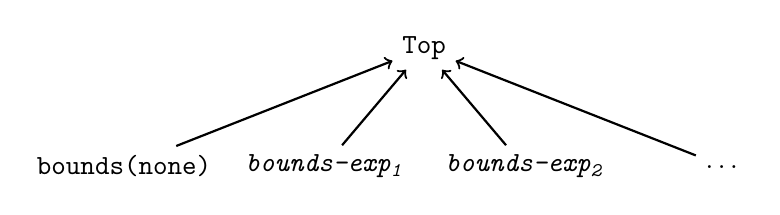
\begin{tikzpicture}[sibling distance=1in]
\node[rectangle, minimum size=8pt]{\texttt{Top}}
  child foreach \name in {\boundsnone, \var{bounds-exp\textsubscript{1}},
                          \var{bounds-exp\textsubscript{2}}, \ldots}
     {node{\name} edge from parent[<-, thick]};
\end{tikzpicture}
\end{center}
\caption{The lattice of values used in dataflow computation of extent}
\label{fig:extent-dataflow-lattice}
\end{figure}
 
For an assignment to an \arrayptr\ variable, the existing
lattice value for the \arrayptr\ variable is killed, unless
the special conditions described in Section~\ref{section:extent-of-declarations}
are met. 
A new lattice value is generated for the \arrayptr\ variable. If the
assignment declares bounds for the \arrayptr\ variable, the new
lattice value is the bounds expression in the bounds declaration.
Otherwise, it is the value \boundsnone.

A declaration of a variable is handled similarly to an assignment,
except that there will not be any lattice value to kill. Lexical hiding
of variables involved in bounds declarations is not permitted. If the
declaration declares bounds for the \arrayptr\ variable, the
new lattice value is the bounds expression in the bounds declaration.
Otherwise, it is the value \boundsnone.

A variable going out of scope kills any existing lattice values in which
that variable occurs.

At control-flow split points, the lattice values for the
\arrayptr\ variables flow to all branches of the split. The
propagation is dataflow-sensitive but not control-flow sensitive. At
control-flow join points, the lattice values are unioned (moving upward
in the lattice). If the lattice values for an \arrayptr\
variable are not the same, the resulting value is \texttt{Top}.

\section{Bounds declarations and loops}

Loops often operate on variables declared outside of loops. They may
read the variables and then update the variables. When these variables
are \arrayptr\ variables they must have bounds and the bound
must be loop invariants.

The common case is that the bounds expression is invariant across all
iterations of the loop. The earlier \texttt{sum} example illustrates
this. The variable \texttt{current} is declared with bounds before a
loop. The loop modifies \texttt{current}, but the bounds for
\texttt{current} do not change:

\begin{verbatim}
/* sum integers stored between start and end, where end is not included */
int sum(array_ptr<int> start where start : bounds(start, end), array_ptr<int> end)
{ 
    int sum = 0;
    array_ptr<int> current : (start, end) = start;

    while (current < end) {
       sum = *current;
       current += 1; // bounds do not need to be redeclared here.
    }
}
\end{verbatim}

A programmer can declare bounds expressions that change on each
iteration of the loop. This may be necessary if an \arrayptr\
variable is modified to point to different memory during a loop
iteration. It also may be desirable for performance reasons. In either
case, there needs to be a loop-invariant bounds declaration.

The following example illustrates this. It is an implementation of
lexicographic comparisons of two arrays, using one pointer to scan each
array. The bounds at the variable declarations serve as loop invariant
bounds. The lower bounds for a variable are declared using the variable
itself, to reduce register pressure in the loop. This can enable
compilers to generate better code. Note that an optimizing compiler will
eliminate the runtime bounds checks easily.

\begin{verbatim}
/* lexicographic comparison of two arrays of integers */
int compare(array_ptr<int> x : bounds(x, x_end), 
            array_ptr<int> y : bounds(y, y_end)
            array_ptr<int> x_end, array_ptr<int> y_end)
{ 
    while (x < x_end && y < y_end) {
        if (*x == *y) {  // bounds check: x >= x && x < x_end; easily optimizable
                         // bounds check: y >= y && y < y_end; easily optimizable
            x++;
            y++;
        }
        else if (*x < *y) {  // bounds checks here are easily optimizable as well
            return -1;
        }
        else {
            return 1;
        }
    }
    if (x == x_end && y == y_end) {
        return 0;
    }
    else if (x != x_end) {
        return 1;
    }
    else {
        return -1; 
    }
}
\end{verbatim}


% !Tex root = checkedc.tex

\chapter{Checking validity of bounds for variables}
\label{chapter:checking-bounds}

This chapter describes basic rules for determining the validity of
bounds declarations in a C translation unit. In general, these rules do
not include any inference steps. Inference steps for reasoning about
bounds are described in Chapter~\ref{chapter:simple-invariants}.

Section~\ref{section:inferring-expression-bounds}
describes how to determine the bounds for an expression of
type \arrayptr\ that does not have any assignments within it.
We start with a set of bounds that are true about variables before the
evaluation of the expression, called the context, and describe the
bounds for the value of the expression.
Section~\ref{section:checking-assignment-expressions}
then describes handling assignment expressions, assuming
that no assignments are nested within the expression. For an assignment
expression, we must determine the updated context in addition to the
value of the expression. The updated context contains new bounds for any
variables assigned to by the expression.
Section~\ref{section:checking-nested-assignment-expressions}
combines the concepts and describes handling expressions
with nested assignments expressions.
Section~\ref{section:checking-expression-statements} 
describes how to validate expression statements. 
Section~\ref{section:checking-function-call-arguments}
describes validating function call arguments.

Because this section covers bounds for \arrayptr\ variables,
not data structures with \arrayptr\ data, certain expressions
are not covered here. This includes member references and expressions
that load or store \arrayptr\ values through pointers. These
expressions are covered in Chapters~\ref{chapter:structure-bounds} and
\ref{chapter:pointers-to-data-with-arrayptrs}.
Section~\ref{section:bounds-checking-indirections} does discuss how to 
insert bounds checking at uses of the
indirection operator (\texttt{*}). This is different than discussing the
bounds of the values \emph{returned} or \emph{stored} through the
indirection operator.

\section{Reducing the number of syntactic cases}

To simplify checking, in-line return bounds expressions are replaced
with the form that uses a name for the return value. The form
\boundsdecl{\var{f}(\ldots{})}{\var{e1}} is changed to 
\texttt{\var{f}(\ldots{}) \keyword{where}
  \boundsdecl{\texttt{return\_value}}{e1}}.
The \texttt{count} and
\texttt{byte\_count} bounds expressions are also expand to bounds expressions.
The form \boundsdecl{\var{x}}{\boundscount{\var{e1}}}
is replaced with \boundsdecl{\var{x}}{\bounds{\var{x}}{\var{x} \texttt{+} \var{e1}}}
and \boundsdecl{\var{x}}{\boundsbytecount{\var{e1}}}
is replaced with \boundsdecl{\var{x}}{\bounds{(\arrayptrchar) \var{x}}{(\arrayptrchar)
\var{x} + \var{e1}}}. For now, we ignore the
additional side conditions on count expressions. Checking of these
conditions will be addressed in Chapter~\ref{chapter:simple-invariants}.

Finally, relative alignment is made explicit for all bounds
declarations: \boundsdecl{\var{x}}{\bounds{\var{e2}}{\var{e3}}} is expanded to
\boundsdecl{\var{x}}{\boundsrelval{\var{e2}}{\var{e3}}{\texttt{sizeof(typeof(\var{x}))}}}.
For code without explicit or implicit casts of \arrayptr s, relative
alignment can be ignored.

In the rules below, we sometimes use shorter syntactic forms for
brevity. The shorter forms should be replaced with the full forms before
using the rules.

\section{Inferring valid bounds for expressions without nested assignment expressions}
\label{section:inferring-expression-bounds}

We first discuss determining valid bounds for expressions that do not
have assignment expressions nested within them. The bounds for an
expression is always determined with respect to a context (bounds for
variables read by the expression). We will use $\vdash$ to denote the
valid bounds for an expression. The notation \boundsinfer{\var{e}}{\var{bounds-exp}}
means that expression \var{e} has valid bounds \var{bounds-exp}.

At times, we need to discuss bounds that are given in terms of the value
of the current expression. For example, a function call expression may
return an \arrayptr\ pointer to an array of constant size
\var{n}. The bounds for that pointer value would be (the
\arrayptr\ pointer, the \arrayptr\ pointer +
\var{n}). We use the special variable \texttt{current\_expr\_value} to
denote the ``current value of the expression.''\footnote{We are open to
  suggestions on the name for this special symbol. We considered the
  term `self', but chose not to use because it is anthromorphic and not
  particularly descriptive. We also considered the term `this', but that
  has specific meaning to programmers who also use object-oriented
  languages, so it is likely to cause confusion.} The bounds for an
expression may involve using the bounds for a subexpression where the
special variable \texttt{current\_expr\_value} occurs. If the ``current
value'' of the expression changes, the uses of
\texttt{current\_expr\_value} from subexpressions must be adjusted to
counter the change. Bookkeeping rules for making this adjustment will be
described in sections that treat expressions with subexpressions.

\subsection{Null pointers}

The bounds for 0 is the \texttt{any} bounds:

\boundsinfer{0}{\boundsany}

\subsection{Variables}
\label{section:checking-variables}

Suppose there is a use of some variable \var{x}.

\begin{itemize}
\item
  If \var{x} has type \arrayptr, the bounds are the result of
  the analysis in Section~\ref{section:extent-definition}
  for this occurrence of \var{x}.
\item
  If \var{x} has type \ptrT, 
  \boundsinfer{\var{x}}{\boundsrel{\var{x}}{\var{x} \texttt{+ 1}}{\var{T}}}.
   On the right-hand side, \var{x} is reinterpreted as having \arrayptr\ type.
\item
  If \var{x} has type
  \spanptrT, 
  \boundsinfer{\var{x}}{\boundsrel{\var{x}\texttt{.lower\_bound}}
                                  {\var{x}\texttt{.upper\_bound}}
                                  {\var{T}}}
\item
  If \var{x} has an array type with a known number of elements \var{n}
  such that the variable is being converted implicitly to a pointer
  type, the bounds are  \boundsinfer{\var{x}}{\boundscount{\var{n}}}.
\item
  Otherwise \var{x} has \boundsnone.
\end{itemize}


\subsection{Addresses of variables}

A variable with type \var{T} whose address is taken is considered to be
an array of one element:

\boundsinfer{\texttt{\&\var{x}}} 
            {\boundsrel{\texttt{\&\var{x}}}{\texttt{\&\var{x} + 1}}{\var{T}}}.

\subsection{Function calls}
\label{section:inferring-bounds-for-function-calls}

Let \var{f} be the name of a function that returns an
\arrayptr\ value (pointers to functions will be handled later).
Suppose there is a function call expression of the form
\var{f}\texttt{(}\var{e1 \ldots{} en}\texttt{)}:

\begin{enumerate}
\item
  If \var{f} has a bounds declaration for the return value of the form
  \texttt{return\_value :} \var{exp1}, then

  \begin{itemize}
  \item
    Any arguments that correspond to formal parameters occurring in
    \var{exp1} must be valid non-modifying expressions. If they are
    not, \boundsinfer{\var{f}\texttt{(\var{e1} \ldots{} \var{en})}}{\boundsnone}.
  \item
    Otherwise, substitute \texttt{\var{e1} \ldots{} \var{en}} for the formal
    parameters of \var{f} occurring in \var{exp1}. Also substitute the
    special symbol \exprcurrentvalue\ for
    \texttt{return\_value}. These substitutions produce \var{exp2}.
    \boundsinfer{\var{f}\texttt{(\var{e1} \ldots{} \var{en})}}{\var{exp2}}.
  \end{itemize}
\item
  If \var{f} does not have a bounds declaration for its return value,
  then \boundsinfer{\var{f}\texttt{(\var{e1} \ldots{} \var{en})}}{\boundsnone}.
\end{enumerate}

The special variable \texttt{return\_value} may appear \var{exp1}. It
is the value of the function call expression, so it is replaced with the
special variable \exprcurrentvalue.

There needs to be validation that the bounds for argument expressions
match the required bounds for formal parameters. This is described in
Section~\ref{section:checking-function-call-arguments}.

The following code provides examples of function call expressions where
bounds need to be computed. In the code, the programmer wraps a call to
\texttt{malloc} in an allocation helper, \texttt{alloc\_helper}. The
function \texttt{alloc\_helper} returns an \arrayptr\ value
that is passed as an argument to \texttt{init}, which initializes the array
and returns the \arrayptr\ value.
\begin{verbatim}
array_ptr<int> alloc_helper(int n) : count(n)
{
    array_ptr<int> result : count(n) = malloc((sizeof(int) * n);
    return result;
}

array_ptr<int> init(array_ptr<int> target : count(s), 
                    int s) : count(s)
{
    for (int i = 0; i < count; i++) {
         target[i] = i;
    }

    return target;
}

void go(int size) 
{
    array_ptr<int> x : count(size) = init(alloc_helper(size), size);
    ...
}
\end{verbatim}

First, syntactic forms for bounds expressions are expanded to eliminate
count expressions and in-line return expressions, as well as make
relative alignment explicit.

\begin{verbatim}
array_ptr<int> alloc_helper(int n)
where return_value : bounds(return_value, return_value + n) rel_align(int)
{
       array_ptr<int> result : bounds(result, result + n) rel_align(int) =
         malloc((sizeof(int) * n);
       return result;
}

array_ptr<int> init(array_ptr<int> target : bounds(target, target + s) rel_align(int), 
                    int s) 
where return_value : bounds(return_value, return_value + s) rel_align(int)
{
    for (int i = 0; i < count; i++) {
         target[i] = i;
    }

    return target;
}

void go(int size) 
{
    array_ptr<int> x : bounds(x, x + size) rel_align(int) = 
      init(alloc_helper(size), size);
    ...
}
\end{verbatim}

The valid bounds for the call to \texttt{init(alloc\_helper(size),
size)} in \texttt{go} are computed using the return bounds for
\texttt{init}:

\begin{verbatim}
    return_value : bounds(return_value, return_value + s) rel_align(int)
\end{verbatim}

First, there is a check that all the actual arguments corresponding to
the formal parameters used by the return bounds expression are valid
non-modifying bounds expressions. This check succeeds even though the
first actual argument \texttt{alloc\_helper(size)} is not a valid bounds
expression. The formal parameter \texttt{target} is not used by the
return bounds expression.

Next, the actual arguments are substituted for the formal parameters and
\exprcurrentvalue\ is substituted for \texttt{return\_value}.
The argument \texttt{size} is substituted for \texttt{s}, producing
\begin{alltt}
    init(alloc\_helper(size), size) \(\vdash\) 
        bounds(\exprcurrentvalue, \exprcurrentvalue + size) rel_align(int)
\end{alltt}

It would not be possible to represent the bounds if \texttt{size} were a
function call too:
\begin{verbatim}
    array_ptr<int> x = init(alloc_helper(getsize()), getsize());
\end{verbatim}

Function calls are not valid in bounds expressions:

\begin{verbatim}
    bounds(expr_current_value, current_expr_value + getsize())  // illegal
\end{verbatim}

The solution would be to assign the result of \texttt{getsize(}) to a
variable:
\begin{verbatim}
   int tmp = getsize();
   array_ptr<int> x = init(alloc_helper(tmp), tmp);
\end{verbatim}

The parameters to the call to \texttt{init} also need to be validated
(see Section~\ref{section:checking-function-call-arguments}). This
requires determining the valid bounds for \texttt{alloc\_helper(size)}. The
return bounds for \texttt{alloc\_helper} are used:
\begin{verbatim}
   return_value : bounds(return_value, return_value + n) rel_align(int)
\end{verbatim}

First, there is a check that the actual arguments that correspond to
formal parameters used in the return bounds are valid non-modifying
expressions. The only argument is the variable size, so this check
succeeds. Next, \texttt{size} is substituted for \texttt{n} and
\exprcurrentvalue\ is substituted for \texttt{return\_value}, producing:
\begin{alltt}
   alloc\_helper(size) \(\vdash\) bounds(\exprcurrentvalue, \exprcurrentvalue + size) 
                         rel_align(int)
\end{alltt}

\subsection{Pointer arithmetic}

The range of memory accessible through pointer arithmetic expressions
remains unchanged from the underlying pointer. In other words, for
\boundsinfer{\var{x}}{\var{bounds-exp}}, the bounds expression for any
pointer arithmetic involving \var{x} is the same as the one for
\var{x}. This is because that C semantics for pointer arithmetic is
that if \var{x} points to an object at runtime, any pointer arithmetic
involving \var{x} must produce a pointer to the same object. The bounds
of the object in memory are not changed by the pointer arithmetic.

We first cover the typical situation where the relative alignment type
for a pointer in a pointer operation matches the referent type of the
pointer. Given a pointer operation of the form \var{x op e1}, where [var{x}
has an \arrayptr\ type, \var{e1} has an integral type, and
\var{op} is addition or subtraction, the memory that can be accessed
through \var{x op e1} is the same memory that can be accessed through
\var{x}:

\begin{itemize}
\item
  If \var{x} is a pointer to \var{T} and 
  \boundsinfer{\var{x}}{\boundsrel{\var{e2}}{\var{e3}}{\var{T}}},
  then \boundsinfer{\var{x} \var{op} \var{e1}}{\boundsrel{\var{e2}}{\var{e3}}{\var{T}}}.
\end{itemize}

This can be extended to pointer operations of the form \var{e4 op e1},
where \var{e4} has type
\arrayptrT\ as
follows:

\begin{itemize}
\item
  If \var{e4} is a pointer to \var{T} and 
  \boundsinfer{\var{e4}}{\boundsrel{\var{e2}}{\var{e3}}{\var{T}}}
  then \boundsinfer{\var{e4 op e1}}{\boundsrel{\var{e2}}{\var{e3}}{\var{T}}}
\end{itemize}

Here is the full rule that handles the situation where the relative
alignment of the pointer differs from the size of the referent type of
the pointer. GCD computes the greatest common divisor of two integers.
The prior rules are just special cases of this rule:

\begin{quote}
If \var{e4} is a pointer to \var{T} and 
\boundsinfer{\var{e4}}
            {\boundsrel{\var{e2}}
                       {\var{e3}}
                       {\var{c}}}
then \boundsinfer{\var{e4 op e1}}
                 {\boundsrel{\var{e2}}
                            {\var{e3}}
                            {\texttt{GCD(\var{c}, sizeof(\var{T}))}}}.
\end{quote}

\subsubsection{Pointer arithmetic for unchecked pointer types}

Pointer arithmetic involving an \arrayptr\ value checks that
the value is non-null and generates a runtime error if it is. This check
is important because a null pointer may have invalid bounds (this
follows from the definition of the meaning of bounds in 
Section~\ref{section:bounds-declarations}). It
prevents a null pointer that has invalid bounds from being used to create a
non-null pointer with valid bounds, which could then be used to access
memory.

Because the meaning of unchecked pointers has not changed, pointer
arithmetic involving a null unchecked pointer may not generate a runtime
error. The rules for array\_ptr pointer arithmetic can be applied to
unchecked pointer arithmetic, however, provided that a side condition that
the pointer expression is non-null is added:

\begin{quote}
If \var{e4} is a pointer to \var{T} and it can be proved that
\var{e4} \texttt{!= 0} and 
\boundsinfer{\var{e4}}{\boundsrel{\var{e2}}{\var{e3}}}{\var{c}}, then
\boundsinfer{\var{e4 op e1}}{\boundsrel{\var{e2}}{\var{e3}}
                                            {\texttt{gcd(\var{c},\sizeof{\var{T}})}}}.
\end{quote}

Chapter~\ref{chapter:simple-invariants}
provides a general framework for checking side-conditions as
part of checking bounds declarations.

\subsubsection{Treatment of expr\_current\_value}

If the special variable \exprcurrentvalue\ occurs in
\bounds{\var{e2}}{\var{e3}}, then
\exprcurrentvalue\ must be adjusted as follows:

\begin{itemize}
\item
  If \var{op} is \texttt{+}, substitute \texttt{\exprcurrentvalue\ -}
  \var{e1} for all occurrences of \exprcurrentvalue\ in
  \bounds{\var{e2}}{\var{e3}}
\item
  If \var{op} is \texttt{-}, substitute \texttt{\exprcurrentvalue\ +}
  \var{e1} for all occurrences of \exprcurrentvalue\ in
  \bounds{\var{e2}}{\var{e3}}.
\end{itemize}

The reasoning behind this is that the current value of the expression has
changed as the result of \var{op} \var{e1}. An adjustment in the
opposite direction of equal magnitude must be made for occurrences of
\exprcurrentvalue.

The following example illustrates the treatment of
\exprcurrentvalue. Consider the prior example that had a
function called \texttt{alloc\_helper} that returned some
newly-allocated memory. Suppose there is an expression that offsets a
pointer returned by a call to \texttt{alloc\_helper}.

\begin{verbatim}
   alloc_helper(size) + 2
\end{verbatim}

To compute the bounds for this expression, first the valid bounds for
\texttt{alloc\_helper(size)} are computed:

\begin{alltt}
   alloc\_helper(size) \(\vdash\) bounds(\exprcurrentvalue, \exprcurrentvalue + size)
\end{alltt}

Next, \texttt{\exprcurrentvalue\ - 2} is substituted for
\exprcurrentvalue\, yielding:

\begin{alltt}
   alloc\_helper(size) + 2 \(\vdash\) (\exprcurrentvalue - 2, \exprcurrentvalue - 2 + size)
\end{alltt}

Now, suppose the pointer is being adjusted to insert some blank padding
at the beginning of the newly-allocated object. We can remove the
occurrence of \texttt{\exprcurrentvalue\ - 2} in the upper bound by
over-allocating in the expression:

\begin{alltt}
   alloc_helper(size + 2) + 2
\end{alltt}

The valid bounds for \texttt{alloc\_helper(size + 2)} are:

\begin{alltt}
   alloc\_helper(size + 2) \(\vdash\) bounds(\exprcurrentvalue, \exprcurrentvalue + size + 2)
\end{alltt}

The valid bounds for the entire expression are:

\begin{alltt}
    alloc\_helper(size + 2) + 2 \(\vdash\) bounds(\exprcurrentvalue - 2,
                                        \exprcurrentvalue - 2 + size + 2)
\end{alltt}

which can be simplified to:

\begin{alltt}
    alloc\_helper(size + 2) + 2 \(\vdash\) bounds(\exprcurrentvalue - 2, 
                                        \exprcurrentvalue + size)
\end{alltt}

As we will explain in Chapter~\ref{chapter:simple-invariants}, 
it is fine to narrow a bounds by
adding a positive constant to the lower bounds. This allows us to adjust
the bounds to what would be desired when extra padding is inserted:

\begin{alltt}
    alloc\_helper(size + 2) + 2 \(\vdash\) bounds(\exprcurrentvalue, 
                                        \exprcurrentvalue + size)
\end{alltt}

\subsection{Cast expressions}
\label{section:cast-expressions}

Given a cast expression of the form \texttt{(\var{T})} \var{e},
the bounds for \var{e} are determined. The bounds for
\var{e} are used as the bounds for the entire expression.

If the special variable \exprcurrentvalue\ appears in the
bounds for \var{e},

\begin{itemize}
\item
  If T is an integral type large enough to hold a pointer or a pointer
  type, let \var{S} be the type of \var{e}. The expression
  \texttt{((\var{S}) \exprcurrentvalue)} is substituted for
  all occurrences of \exprcurrentvalue.
\item
  Otherwise, the bounds of \var{e} are  altered to \boundsnone.
\end{itemize}
  
\subsection{Conditional expressions}

Given an expression of the form \var{e1} \texttt{?} \var{e2}
\texttt{:} \var{e3}, the bounds for \var{e2} and \var{e3} are
determined. They must be syntactically identical (after putting the
bounds into a normal form). The bounds for \var{e2} are used as the
bounds for the entire expression.

If the special variable \exprcurrentvalue\ occurs in the
bounds for \var{e2}, it is left unchanged. The conditional expression
does not change the value returned by one if its branches, so no
adjustment to \exprcurrentvalue\ is needed.

\emph{This is an expression where a conditional bounds expression could
be used to represent the resulting range.  Another alternative that works
with current syntax would be to create upper/lower-bound expressions
that use e1 such as (e1 ? lower-bound(e2) : lower-bound(e3), e1 ?
upper-bound(e2) : upper-bound(e3). For now, we defer discussion of both
alternatives. }

\subsection{Comma expressions}

Given an expression of the form \var{e1} \texttt{,} \var{e2}, the
bounds for \var{e2} are determined. The bounds for \var{e2} are used
as the bounds for the entire expression.

If the special variable \exprcurrentvalue\ occurs in the
bounds for \var{e2}, it is left unchanged.

\section{Bounds for assignment expressions}
\label{section:checking-assignment-expressions}

For an assignment expression of the form \var{x} \texttt{=} \var{e},
where \var{x} is a variable and \var{e} is an expression, we start
with a context that is true before the evaluation of the assignment
expression. We determine the context that will be true after the
evaluation of the assignment expression and the bounds for the value
returned by the assignment expression.

This seems straightforward at first. If \var{x} has type
\arrayptr, compute the bounds for \var{e} and update the
context so that the bounds for \var{x} is the bounds of \var{e}.
However, there is a problem. The bounds for \var{e} is determined
\var{before} \var{x} changes value. When \var{x} changes value, the bounds
for \var{e} may no longer be true if \var{x} appears in the bounds.
The context could contain uses of \var{x} also in bounds expressions.

A simple solution is to invalidate bounds expressions where x appears in
the bounds. This does not work well when a variable that appears in its
own bounds declaration is incremented or decremented. Consider the
following example:
\begin{verbatim}
array_ptr<int> x : bounds(x, high) = ...
int sum = 0;
while (x < high) {
    sum += *x;
    x++;  // bounds for x would be undefined for the simple solution
}
\end{verbatim}

A possible solution is to require programmers to copy variables in loops
that are modified using only pointer arithmetic to temporary variables
before the loop. The temporary variables could then be used in bounds.
However, this might increase register pressure and worsen performance.

One can do better than that for loop induction variables, which are
variables that are incremented or decremented by a constant in a loop.
Condit \textit{et al.} observe that some assignment expressions are
invertible: the old value of a variable can be calculated from the new
value . One can update the bounds by substituting the inverted
expression in place of the variable. The updated bounds can then be
narrowed to satisfy loop bounds invariants. Invertible expressions
include the addition and subtraction expressions that update loop
induction variables.

The updated context will be determined in three steps. First, if
\var{x} has type \arrayptr, the context is updated for
\var{x} using bounds expressions that use the \emph{old} value of \var{x}:

\begin{enumerate}
\item
  If \boundsinfer{\var{e}}{\var{exp}}, then the context is updated with
  \boundsdecl{\var{x}}{\var{exp}}.
\item
  Otherwise, the context is updated with \boundsdecl{\var{x}}{\boundsnone}
   to indicate that \var{x} has no valid bounds.
\end{enumerate}

Second, the context is updated to reflect the change in the value of
\var{x}:

\begin{itemize}
\item
  If the expression being assigned is invertible, the right-hand side of
  any bounds expression that uses \var{x} will be updated to use an
  expression that inverts the new value to compute the old value.
\item
  Otherwise, any bounds expression that involves x is invalidated
\end{itemize}

An assignment expression in C has a value. The bounds of the assignment
expression will be the bounds of \var{x} at this point.

Third, the special variable \exprcurrentvalue\ is eliminated
from the bounds of \var{x}, if it was introduced because it occurred in
\boundsdecl{\var{e}}{\var{exp}}. Recall that
\exprcurrentvalue\ stands for the current value of an
expression whose bounds is being determined. Because the value of
\var{e} has been assigned to \var{x}, \var{x} is substituted for
\exprcurrentvalue\ in the bounds for x.

\subsection{Invertibility}

The following examples illustrate invertibility and updating bounds. For
the first example, suppose there is a declaration of an
\arrayptr\ variable followed by a decrement of a variable
involved in the bounds:

\begin{verbatim}
array_ptr<int> a : count(len) = ...
len = len - 1
\end{verbatim}

The original value of \texttt{len} can be computed from the new value.
In this case, a valid new bounds after the decrement of \texttt{len} is
\texttt{count(a) == len + 1.} The bounds for \texttt{a} after the
assignment are:
\begin{verbatim}
len = len - 1
where a : count(len + 1);
\end{verbatim}

For the second example, consider an update to a pointer variable that
appears in its own bounds:
\begin{verbatim}
array_ptr<int> p : bounds(p, high) = ...         
while (p < high) {
    ...
          p = p + 1;
}
\end{verbatim}

First, the new bounds expression for the expression \verb|p + 1| is
computed. It is the same as the original bounds expression
\verb|bounds(p, high)|. Because p is modified by the assignment, the
inverted expression for \verb|p + 1| is substituted into 
\verb|(p, high)|. The inverted expression for \verb|p + 1| is \verb|p - 1|.
Substituting \verb|p-1| for \verb|p| leads to bounds of the form
\verb|bounds(p - 1, high)|:

\begin{verbatim}
while (p < high) {
    ...
          p = p + 1 where p : bounds(p - 1, high);
}
\end{verbatim}

Bounds ty is preserved when the range of a bounds expression is
narrowed. \texttt{(p - 1, high)} implies that \texttt{(p, high)} is a
valid bounds expression. This reestablishes the loop bounds invariant
for \texttt{p} of \texttt{(p, high)}.

\begin{verbatim}
while (p < high) {
    ...
          p = p + 1 where p : bounds(p, high);
}
\end{verbatim}

The correctness of narrowing depends on pointer arithmetic overflow
for checked pointer types being a runtime error. For a lower bound \var{e1} in a bounds
expression, we can only substitute \var{e2} for \var{e1} as the lower
bound if \var{e2} \textgreater{}= \var{e1}. The identity \texttt{p > p - 1} 
holds only if overflow is a runtime error.

\subsection{Invertible expressions}
An expression is invertible with respect to a variable x if:

\begin{enumerate}
\item
  The expression is x
\item
  or

  \begin{enumerate}
  \item
    The operator in the expression is an addition, subtraction, one's
    complement, unary minus, unary plus, exclusive-or, a bit-preserving
    cast operator, or a widening cast operator, and
  \item
    The variable x occurs only in one argument of the operation and that
    argument is an invertible expression with respect to \var{x}
  \item
    Any other argument of the operation is a non-modifying expression,
    excluding non-modifying expressions that are or include member
    references, indirect member references, or pointer dereferences.
  \end{enumerate}
\end{enumerate}

The addition and subtraction operations must be for checked pointer
arithmetic or unsigned integer arithmetic. An implementation may allow
integral addition and subtraction operations to be invertible if
integral addition and subtraction are defined as two's complement
arithmetic where extra bits are discarded on overflow. However, this
introduces the possibility of non-portable code.

Given the expression \texttt{x =} \var{e}, where \texttt{x} occurs once
in \var{e}, mathematical rules are applied to solve for \texttt{x} in
\var{e}. We generalize the left-hand side from x to an expression
\var{f} and define \texttt{inverse(}\var{f}\texttt{,}
\var{e}\texttt{)} as follows:

\begin{longtable}[c]{@{}ll@{}}
\toprule
\texttt{Given inverse(}\var{f}\texttt{,} \var{e}\texttt{), where} &
\texttt{the result is:}\tabularnewline
\midrule
\endhead
\var{e} = \texttt{x} & \var{f}\tabularnewline
\var{e} = \texttt{\textasciitilde{}}\var{e1} &
\texttt{inverse(\textasciitilde{}}\var{f},
\var{e1}\texttt{)}\tabularnewline
e = \texttt{-}\var{e1} & \texttt{inverse(-}\var{f},
\var{e1}\texttt{)}\tabularnewline
\var{e} = \texttt{+}\var{e1} & \texttt{inverse(+}\var{f},
\var{e1}\texttt{)}\tabularnewline
\var{e} = \texttt{(}\var{t1}\texttt{)} \var{e1}, where \var{e1} has
type \var{t2} & \texttt{inverse((}\var{t2}\texttt{)} \var{f},
\var{e1}\texttt{)}\tabularnewline
and \texttt{(\var{t1})} is not a narrowing cast & \\
\var{e} = \var{e1} \texttt{+} \var{e2}, where \texttt{x} occurs in
\var{e1} & \texttt{inverse(}\var{f} \texttt{-} \var{e2},
e1)\tabularnewline
\var{e} = \var{e1} \texttt{+} \var{e2}, where \texttt{x} occurs in
\var{e2} & \texttt{inverse(}\var{f} \texttt{-} \var{e1},
\var{e2})\tabularnewline
\var{e} = \var{e1} \texttt{-} \var{e2}, where \texttt{x} occurs in
\var{e1} & \texttt{inverse(}\var{f} \texttt{+} \var{e2},
\var{e1})\tabularnewline
\var{e} = \var{e1} \texttt{-} \var{e2}, where \texttt{x} occurs in
\var{e2} & \texttt{inverse(}\var{e1} \texttt{-} \var{f},
\var{e2})\tabularnewline
&\tabularnewline
\var{e} = \var{e1} \texttt{\^{}} \var{e2}, where \texttt{x} occurs in
\var{e1} & \texttt{inverse(}\var{f} \texttt{\^{}} \var{e2},
\var{e1})\tabularnewline
\var{e} = \var{e1} \texttt{\^{}} \var{e2}, where \texttt{x} occurs in
\var{e2} & \texttt{inverse(}\var{f} \texttt{\^{}} \var{e1},
\var{e2})\tabularnewline
\bottomrule
\end{longtable}

Given \texttt{inverse(x}, \var{e}), the rules are applied repeatedly
until the original value of x in e has been computed. Here is an example
of computing the inverse of \texttt{x = (x + 4) + 5}:
\begin{verbatim}
   inverse(x, (x + 4) + 5) =
       inverse(x - 5, x + 4) =
          inverse((x - 5) - 4, x) =
              (x - 5) - 4
\end{verbatim}

\section{Bounds for expressions with nested assignment expressions}
\label{section:checking-nested-assignment-expressions}

C allows assignment expressions to be nested within other expressions.
This means that the approach of 
Section~\ref{section:checking-assignment-expressions} has to be extended to walk
expressions recursively and update the context during the walk.

Given some expression e that has subexpressions e\textsubscript{1}
\ldots{}. e\textsubscript{n}, start with the context for e. Compute a
new context and the bounds expression for e as follows:

\begin{itemize}
\item
  Traverse e\textsubscript{1} \ldots{} e\textsubscript{n} in an order
  that respect the sequence points of \cite{ISO2011}. For each subexpression, take the
  context and compute the updated context and the bound expression (if
  any) for the subexpression.
\item
  If e is an assignment expression, 
  apply the rules in Section~\ref{section:checking-assignment-expressions} to
  compute an updated context and a bounds expression for e
\item
  Otherwise, apply the rules in Section~\ref{section:inferring-expression-bounds}
  to compute an updated bounds
  expression for e.
\end{itemize}

\section{Expression statements}
\label{section:checking-expression-statements}

Expression statements need to be checked for consistency with their
expected bounds declarations. If an expression statement is within a
bundled block, the checking is deferred to the end of the bundled block.

To check an expression statement, the analysis of 
Section~\ref{section:extent-definition} is used
to determine the context for the expression in the statement (the bounds
for variables before the statement is evaluated). The rules in 
Section~\ref{section:checking-nested-assignment-expressions}
are then used to determine the updated context.

The updated context is then checked against the bounds declarations that
must be true after the expression statement. For each
\arrayptr\ variable \var{x} in scope, the expected bounds is
computed:

\begin{itemize}
\item
  If the expression statement has a bounds declaration for \var{x}, the
  bounds expression in that bounds declaration is used.
\item
  Otherwise, the analysis of Section~\ref{section:extent-definition}
  is used to determine the
  expected bounds expression for x.
\end{itemize}

We will refer to the bounds expression for \var{x} in the updated context
as the updated bounds expression.  It must imply that the
expected bounds expression holds. Implication is checked in this section
using by placing non-modifying expressions into a canonical form and
checking for syntactic equality. If two expressions have the same
canonical form, any values that they have at runtime will always be
identical. Chapter~\ref{chapter:simple-invariants}
describes more general techniques for checking
that context bounds imply the expected bounds.

The updated bounds expression implies that the expected bounds
expression holds if:

\begin{itemize}
\item
  The expected bounds expression is \boundsnone, or
\item
  The updated bounds expression is \boundsany, or
\item
  The updated bounds expression and the expected bounds expression are
  equal syntactically after placing the expressions into canonical
  forms,
\item
  The canonicalized expressions
  differ syntactically only in their relative alignment, and
  the context bounds implies the expected relative alignment \var{c}.
  This is true if:

  \begin{itemize}
  \item
    The context relative alignment is an integer multiple of the
    expected relative alignment,
  \item
   or given a context bounds expression of the form
   \boundsrel{\var{e1}}{\var{e2}}{\var{d}},
   \texttt{((\arrayptrchar) \var{x} - (\arrayptrchar) \var{e1}) \% \var{c}}
   canonicalizes to \texttt{0}, as does
   \texttt{((\arrayptrchar) \var{e2} - (\arrayptrchar) \var{x}) \% \var{c}}.
  \end{itemize}
\end{itemize}

\subsection{Canonicalization of expressions in bounds expressions}
\label{section:canonicalization}

Most readers can skip this section safely and come back to it as
necessary. This section is for compiler implementers and for programmers
who want to understand when expressions are regarded as identical by
canonicalization.

Canonicalization guarantees the following: if two non-modifying
expressions have the same canonical form and if they produce values when
evaluated at runtime, the two values will be equal. There are two
important things to understand about this definition. First, two C
expressions may have different canonicalized forms and still always
produce the same value at runtime (in the terminology of logic,
canonicalization is incomplete). Second, canonicalization does not
guarantee that an expression will actually produce a value at runtime.
It may still have a runtime fault. The runtime correctness of bounds
expressions is implied by transitivity: a bounds expression must be
implied by another bounds expression, and so on, until a bounds
expression is implied by an allocation. The allocation must have
involved an expression that actually produced a value.

This has a surprising consequence: integer arithmetic operations that
check for overflow can be regarded as following mathematical rules
during canonicalization. A compiler could not reassociate \texttt{((a
+\textsubscript{ovf} b) +\textsubscript{ovf} c)} to \texttt{(a
+\textsubscript{ovf} (b +\textsubscript{ovf} c)} and replace the first
expression with the second one because it could cause an overflow where
none occurred before. For canonicalization, though, reassociation is
fine.

Signed integer operations do not follow certain mathematical identities.
This is because according to the rules in 
Section~\ref{section:changes-to-undefined-behavior}, they may produce
a value on overflow, but the properties of the value are not specified.
Signed addition is not associative: \texttt{(a + b) + c} is not
guaranteed to produce the same result as \texttt{a + (b + c)} in the
presence of overflow. The expression \texttt{a + b} may overflow, while
\texttt{b + c} may not overflow or the reverse may occur. In addition,
for signed integers, it is not guaranteed that \texttt{a - b} =
\texttt{a + (-b)} or that \texttt{-(-(a))} = \texttt{a}.

The canonicalization rules need to disambiguate between signed and
unsigned operators for integers, as well as operators that check for
overflow. All integer operators will be subscripted by whether they
apply to signed or unsigned integers and whether they check overflow 
using the subscripts \texttt{signed}, \texttt{unsigned}, and
\texttt{ovf}. For example, the expression \texttt{(a + b) + c} involving
signed integers will be written as \texttt{(a
+}\emph{\textsubscript{signed}} \texttt{b)
+}\emph{\textsubscript{signed}} \texttt{c}.

The overflow checking operators introduced in
Section~\ref{section:pointers-as-integers} only include
operators that can occur in practice. For canonicalization, it is useful
to have a complete set of operators, including
\texttt{+\textsubscript{ovf}} and \texttt{\textsubscript{-ovf}} that
take two integers (both signed or unsigned) and produce an integer that
has the same type as the arguments, as well as unary negation that takes
a signed or unsigned integer and produces a signed integer.

In the rules for canoncialization, when a subscript on an integer
operator is omitted, the rule applies to all forms of the operator.
Sometimes the subscript \var{kind} will be used on operators. Either
u\texttt{nsigned} or \texttt{ovf} should be substituted for \var{kind}
in the rule.

The first step in canonicalization is to convert non-modifying
expressions to an initial representation:

\begin{compactenum}
\item
  All expressions involving operators are fully parenthesized and
  unnecessary parenthesis on variables and constants are removed. For
  example, \var{e1} \var{op1} \var{e2} \var{op2} \var{e3}, is
  replaced by \texttt{((}\var{e1} \var{op1} \var{e2}\texttt{)}
  \var{op2} \var{e3}\texttt{)} or \texttt{(}\var{e1} \var{op1}
  \texttt{(}\var{e2} \var{op2} \var{e3}\texttt{))}, depending on the
  precedence of \var{op1} and \var{op2}.
\item
  Implicit cast operations are made explicit.
\item
  The pointer dereference \texttt{*} and pointer indirection operators
  \texttt{(->)} are implicitly annotated with their pointer types.
  This is necessary because converting pointer arithmetic to integer
  arithmetic will erase the type information needed by these operators.
\item
  Unary plus operations are removed.
\item
  Array references of the form
  \var{e1}\texttt{[}\var{e2}\texttt{]} are converted to
  \texttt{*((}\var{e1}\texttt{)} \texttt{+}
  \texttt{(}\var{e2}\texttt{))}
\item
  Pointer arithmetic is expanded to integer-based arithmetic.
\item
  Binary subtraction expressions are canonicalized to use unary minus
  when possible: \var{e1} \texttt{-}\emph{\textsubscript{kind}}
  \var{e2} is converted to \var{e1}
  \texttt{+}\emph{\textsubscript{kind}}
  \texttt{-}\emph{\textsubscript{kind} e2}.
\end{compactenum}

For the second step of canonicalization, two sets of binary arithmetic
operators are defined

\begin{compactitem}
\item
  The set of of commutative and associative operators (CA operators).
  This includes:

  \begin{itemize}
  \item
    The operators +\texttt{\textsubscript{unsigned}},
    \texttt{*\textsubscript{unsigned}}, \texttt{+\textsubscript{ovf}},
    and \texttt{*\textsubscript{ovf}}
  \item
    The bitwise operators \texttt{\textbar{}}, \texttt{\&}, and
    \texttt{\^{}}
  \item
    The Boolean operators \texttt{\textbar{}\textbar{}} and
    \texttt{\&\&}
  \end{itemize}
\item
  The set of commutative-only operators (CO):
  \texttt{+\textsubscript{signed}} and \texttt{*\textsubscript{signed}}.
\end{compactitem}

The following rules are applied until no further changes occur:

\begin{compactenum}
\item
  Removing pointer casts and identity casts on integral types (casts
  from a type to itself). Pointer casts do not change the values of
  pointers.
\item
  Folding constant integral expressions. The following expressions are
  constant-folded:

  \begin{compactenum}
  \item
    Any constant expression that uses only overflow-checking arithmetic
    operators and that mathematically evaluates to an in-range integer
    value. The value is the mathematical result.
  \item
    Any constant expression involving integers that produces a defined
    result according to the C language standard or the C implementation
    rules.
  \end{compactenum}
\item
  Applying algebraic identities to simplify expressions

  \begin{compactenum}
  \item
    Arithmetic identities

    \begin{compactenum}
    \item
      \var{e} \texttt{+} \texttt{0} = \var{e}, \var{e} \texttt{-}
      \texttt{0} = \var{e}, \texttt{0} \texttt{-} \var{e} =
      \texttt{(-}\var{e}\texttt{)}, \texttt{0} \texttt{*} \var{e} =
      \texttt{0}, \texttt{1} \texttt{*} \var{e} = \var{e}, \var{e} /
      \texttt{1} = \var{e}, \var{e}\texttt{/-1} = \texttt{-}\var{e},
      \var{e} \texttt{\%} \texttt{1} = \var{e}
    \item
      For a positive constant \var{c}, (\var{e}
      \texttt{*}\emph{\textsubscript{kind}} \var{c}) \texttt{\%}
      \var{c} = \texttt{0}
    \end{compactenum}
  \item
    Bitwise identities: \var{e} \texttt{\&} \texttt{0} = \texttt{0},
    \var{e} \texttt{\textbar{}} \texttt{0} = \var{e}, \var{e}
    \texttt{\^{}} \texttt{0} = \var{e}, and
    \texttt{\textasciitilde{}(\textasciitilde{}}\var{e}\texttt{))} =
    \var{e}
  \item
    Boolean identities: given a non-zero constant c, \var{e}
    \texttt{\&\&} \var{c} simplifies to \var{e}, \var{e}
    \texttt{\textbar{}\textbar{}} \var{c} simplifies to \texttt{1}, and
    \texttt{!}\var{c} = \emph{0}. When \var{c} = \texttt{0}, \var{e}
    \texttt{\&\&} \var{c} simplifies to \texttt{0}, \var{e}
    \texttt{\textbar{}\textbar{}} \var{c} simplifies to \var{e}, and
    \texttt{!}\var{c} = \texttt{1}.
  \item
    Double negation:
    \texttt{-}\emph{\textsubscript{kind}}(\texttt{-}\emph{\textsubscript{kind}}
    \var{e}\texttt{)} = e.
  \item
    Cancelling terms: \var{e} \texttt{-}\textsubscript{signed} \var{e}
    simplifies to \texttt{0} and \var{e} \texttt{+\textsubscript{kind}}
    (\texttt{-\textsubscript{kind}} \var{e}) simplifies to \texttt{0}.
    This is applied more generally to a sequence of addition operations
    of the form \texttt{(}\ldots{} \texttt{(}e1
    \texttt{+}\textsubscript{kind} e2\texttt{)} \ldots{}
    \texttt{+}\textsubscript{kind} \texttt{-}\emph{\textsubscript{kind}}
    e1 \ldots{}\texttt{)}.

    When identities have commutative versions, those are applied as
    well.
  \end{compactenum}
\item
  Applying associativity commutivity, and distributivity rules to put
  expressions in canonical forms:
\begin{compactenum}
\item
  For each operator \var{op} in CA, repeatedly rewriting any expression
  of the from \var{e1} \var{op} \texttt{(}\var{e2} \var{op}
  \var{e3}\texttt{)} to \texttt{(}\var{e1} \var{op}
  \var{e2}\texttt{)} \var{op} \var{e3} until no further rewrites are
  possible.
\item
  For each operator \var{op} in CA, for each sequence of operations
  (\ldots{} ((\var{e1} \var{op} \var{e2}) \var{op} \var{e3})
  \ldots{} \var{op} \var{en}), reordering the operands so that
  \var{e1} \ldots{} \var{en} appear in lexicographic order. Constants
  should appear lower in the lexicographic order than more complex
  expressions.
\item
  For each operator \var{op} in CO, commuting the operands in \var{e1}
  \var{op} \var{e2} so that \var{e1} is lower in the lexicographic
  order.
\item
  Applying the following distributivity rules:

  \begin{compactenum}
  \item
    Rewriting \texttt{-}\emph{\textsubscript{kind}}\texttt{(}\var{e1}
    \texttt{+}\emph{\textsubscript{kind}} \var{e2}\texttt{)} to
    \texttt{(-}\emph{\textsubscript{kind} e1}\texttt{)} \texttt{+}
    \texttt{(-}\emph{\textsubscript{kind} e2}\texttt{)},
  \item
    Rewriting \texttt{(}\var{e1} \texttt{+}\emph{\textsubscript{kind}}
    \var{e2}\texttt{)} \texttt{*}\emph{\textsubscript{kind}} \var{e3}
    to \texttt{(}\var{e1} \texttt{*}\emph{\textsubscript{kind}}
    \var{e3}\texttt{)} \texttt{+}\emph{\textsubscript{kind}}
    \texttt{(}\var{e2} \texttt{*}\emph{\textsubscript{kind}}
    \var{e3}\texttt{)}
  \item
    Rewriting \texttt{(}e1 \textbar{} e2\texttt{)} \& e3 as \texttt{(}e1
    \& e3\texttt{)} \textbar{} \texttt{(}e2 \& e3\texttt{)} and
    rewriting e3 \& \texttt{(}e1 \textbar{} e2\texttt{)} as \texttt{(}e3
    \& e1 \textbar{} e3 \& e2\texttt{)}
  \item
    Rewriting !(e1 \textbar{}\textbar{} e2) as ((!e1) \&\& (!e2)) and
    !(e1 \&\& e2) as ((!e1) \textbar{}\textbar{} (!e2))
  \item
    Rewriting (e1 \textbar{}\textbar{} e2) \&\& e3 as (e1 \&\& e3)
    \textbar{}\textbar{} (e2 \&\& e3) and rewriting e3 \&\& (e1
    \textbar{}\textbar{} e2) as (e3 \&\& e1 \textbar{}\textbar{} e3 \&\&
    e2)
  \end{compactenum}
\end{compactenum}
\end{compactenum}

The distributivity rules expand the size of expressions, potentially
increasing size exponentially. Implementations may have a reasonable
limit on the size of canonicalized expressions. A minimum required limit
will be determined based on an empirical evaluation of C programs.

\subsection{An example of canonicalization}
\label{section:canonicalization-example}

Here is how bounds for the following declaration and statement will be checked:
\begin{verbatim}
array_ptr<int> x;
x = malloc(sizeof(int)*5) where x : count(5);
\end{verbatim}

The function \verb+malloc+ is assumed to have the bounds declaration:

\begin{verbatim}
array_ptr<void> malloc(size_t num) : byte_count(num);
\end{verbatim}

even though in practice it will have a bounds-safe interface that does
not use a checked pointer type.

First, the implicit casts are made explicit and count is expanded to bounds:

\begin{verbatim}
x = (array_ptr<int>) malloc(sizeof(int)*(size_t) 5) where x : bounds(x, x + 5);
\end{verbatim}

Next, the bounds for the right-hand expression are computed. The bounds
declaration for malloc is expanded to:
\begin{verbatim}
array_ptr<void> malloc(size_t num)  
where return_value : bounds((array_ptr<char>) return_value, 
                            (array_ptr<char>) return_value + num)
\end{verbatim}

The bounds for malloc are used to compute the bounds for the function
call \verb+malloc(sizeof(int)*(size_t) 5)+. The actual argument
\verb+sizeof(int)*(size_t) 5+ is substituted for \verb+num+ in the
bounds expression for the return value of \verb+malloc+:
\begin{verbatim}
return_value : bounds((array_ptr<char>) return_value, 
                      (array_ptr<char>) return_value + sizeof(int)*(size_t) 5)
\end{verbatim}

Next, \verb+expr_current_value+ is substituted for \verb+return_value+ :
\begin{verbatim}
expr_current_value : bounds((array_ptr<char>) expr_current_value, 
                            (array_ptr<char>) expr_current_value + sizeof(int)*(size_t) 5)
\end{verbatim}

Then, the bounds for \verb|(array_ptr<int>) malloc(sizeof(int)*(size_t) 5)|
are computed. The inverse cast \verb|(array_ptr<void> expr_current_value)|
is substituted for \verb|expr_current_value|:

\begin{verbatim}
expr_current_value : bounds((array_ptr<char>) ((array_ptr<void>) expr_current_value), 
                            (array_ptr<char>) ((array_ptr<void>) expr_current_value)
                            + sizeof(int)*(size_t) 5) 
\end{verbatim}

Finally, \verb|x| is substituted for \verb|expr_current_value| :

\begin{verbatim}
x : bounds((array_ptr<char>) ((array_ptr<void>) x), 
           (array_ptr<char>) ((array_ptr<void>) x) + sizeof(int)*(size_t) 5) 
\end{verbatim}

Now, it has be shown that the computed bounds for \verb|x|\ imply the expected
bounds for \verb|x|\ of \verb|bounds(x, x + 5)|. The bounds expressions are both
converted to use integer arithmetic:

\begin{alltt}
// computed bounds
bounds((\arrayptrchar) ((\arrayptrvoid) x),
       (\arrayptrchar) ((\arrayptrvoid) x) +\textsubscript{ovf} sizeof(int)*\textsubscript{unsigned}(size\_t) 5))
// expected bounds
bounds(x, x +\textsubscript{ovf} (5 *\textsubscript{ovf} (signed\_size\_t) sizeof(int)))
\end{alltt}

Next, unnecessary pointer casts are removed:
\begin{alltt}
// computed bounds
bounds(x, x +\textsubscript{ovf} (sizeof(int) *\textsubscript{unsigned} (size\_t) 5))
// expected bounds
bounds(x, x +\textsubscript{ovf} (5 *\textsubscript{ovf} (signed\_size\_t) sizeof(int)))
\end{alltt}

After that, constant folding is done. If \verb+sizeof(int)+ is 4, the result is:
\begin{alltt}
// computed bounds
bounds(x, x +\textsubscript{ovf} 20)
// expected bounds
bounds(x, x +\textsubscript{ovf} 20)
\end{alltt}

We must also show the expected bounds imply that the 
\verb|rel_align(int)| requirement is met. This is straightforward for
a constant-sized array. It involves showing given \bounds{\var{e1}}{\var{e2}}
that \texttt{((\arrayptrchar) x - (\arrayptrchar) \var{e1}) \% 4} canonicalizes
to 0, as does \texttt{((\arrayptrchar) \var{e2} - (\arrayptrchar) x) \% 4}.

For the first expression, \texttt{((\arrayptrchar) x - (\arrayptrchar) x) \% 4}
simplifies to \texttt{0 \% 4}, which constant-folds to \texttt{0}.
For the second expression, \texttt{((\arrayptrchar) (x + 5) - (\arrayptrchar) x) \% 4}
simplifies to \texttt{((x +\textsubscript{ovf} 20) -\textsubscript{ovf\_diff} x) \% 4}. This
simplifies to \texttt{20 \% 4}, which constant-folds to \texttt{0}.

If we change the example to make the number of elements variable instead
of constant, we can see how canonicalization breaks down in the presence
of integer wraparound. Suppose the number of elements is given by a
variable \verb|k|. We would have:

\begin{alltt}
// computed bounds
bounds(x, x +\textsubscript{ovf} (sizeof(int) *\textsubscript{unsigned} (size\_t) k))
// expected bounds
bounds(x, x +\textsubscript{ovf} (k *\textsubscript{ovf} (signed\_size\_t) sizeof(int)))
\end{alltt}

After converting pointer arithmetic to integer arithmetic, we have:
\begin{alltt}
// computed bounds
bounds(x, x +\textsubscript{ovf} (4 *\textsubscript{unsigned} (size\_t) k))
// expected bounds
bounds(x, x +\textsubscript{ovf} (k *\textsubscript{ovf} 4))
\end{alltt}

Canonicalization of the upper bounds expressions produces:
\begin{alltt}
// computed bounds
x +\textsubscript{ovf} (4 *\textsubscript{unsigned} (size\_t) k))
// expected bounds
x +\textsubscript{ovf} (4 *\textsubscript{ovf} k)
\end{alltt}

The expressions are not identically syntactically, so bounds expression
checking fails. The additional side conditions that \verb|k >= 0 && k <= UINTPTR_MAX/4|
are needed to show that the computed upper bound implies the expected upper bound. More
general techniques from Chapter~\ref{chapter:simple-invariants} are needed to show that the context
bounds imply the expected bounds.

\subsection{Extending canonicalization to two's complement signed integer arithmetic}

In some widely-used C compilers, signed arithmetic implemented
as two's complement arithmetic is available under a compiler flag. In
this case, the expected arithmetic properties hold, which enables more
expressions to be canonicalized to the same form.

\section{Declarations}
\label{section:checking-declarations}

Declarations also need to be checked for consistency with their bounds
declarations. If the declaration is within a bundled block, the checking
is deferred to the end of the bundled block.

C distinguishes between declarations and definitions of variables. A
declaration declares the type and storage class for a variable. It may
or may not cause storage to be allocated for the variable. A definition
is a declaration of a variable that causes storage to be allocated for
the variable as well. Definitions may have initializers that initialize
the storage for the variable.

We first describe checking definitions, which is similar to checking
assignments. For a declaration, we assume that there is an ordered list of
\arrayptr\ variables and their optional initializers, and the
list of bounds declarations in the where clause for the declaration. The
list is ordered by the order of variable declarations.

First, the current context is computed before the declaration. Then, for
each variable \var{v} in the list,

\begin{itemize}
\item
  If \var{v} has an initializer, the current context is updated by
  traversing the assignment expressions in the initializer using the
  analysis from Section~\ref{section:checking-nested-assignment-expressions}. 
  The bounds for each individual assignment
  expression are recorded as well. Note that if \var{v} is a static
  variable, the assignment expressions must actually be constant
  expressions, so the context will not change.
\item
  If \var{v} has an \arrayptr\ type or an incomplete array
  type, the context is updated to record the new bounds for \var{v}:

  \begin{itemize}
  \item
    If \var{v} has no initializer, then

    \begin{itemize}
    \item
      If \var{v} is a static variable, then \var{v} will be
      initialized to 0. The context is updated to map \var{v} to
      \boundsany.
    \item
      If \var{v} is an automatic variable then \var{v} will have an
      indeterminate value. The context is updated to map v to
      \boundsnone.
    \end{itemize}
  \item
    If \var{v} has an initializer, the initializer must have the form
    \var{e} or \texttt{\{} \var{e} \texttt{\}}. In both cases,

    \begin{itemize}
    \item
      If \exprcurrentvalue\ appears in the bounds for
      \var{e}, \var{v} is substituted for it.
    \item
      The context is updated to map v to the updated bounds.
    \end{itemize}
  \end{itemize}
\end{itemize}

The current context is then checked against the bounds declarations that
must be true after the declaration using the analysis in 
Section~\ref{section:checking-expression-statements}

Declarations that are not definitions are not checked, other than to
verify that all the declarations of a variable in a translation unit
have the same bounds declaration (or lack of a bounds declarations) for
the variable.

\section{Bundled declarations and statements}
\label{section:checking-bundled}

To check bundled declarations and statements, the current context is
determined before the bundled block. The current context is then updated
for each expression statement and declaration following the rules for
updating contexts in Sections~\ref{section:checking-expression-statements} and 
\ref{section:checking-declarations}. The analysis of 
Section~\ref{section:extent-definition}
is used to determine the expected bounds expression for each variable at
the end of the bundled block. The current context is checked against the
bounds declarations that must be true at the end of the block using the
analysis in Section~\ref{section:checking-expression-statements}

When an expression with \arrayptr\ type is dereferenced within
an expression statement in a bundled block, the current context before
the statement is used to determine the bounds for the expression. This
may cause an expression to have a different bounds than it normally
would have based on bounds declarations.

For example, suppose a pointer assignment is introduced into the middle
of the earlier example. The pointer assignment is highlighted in blue.
The bounds for \verb|parr| at that point in the program based on the
current context will be \verb|bounds(parr, parr + size)|.
\begin{verbatim}
int arr[DEFAULT_SIZE];
array_ptr<int> parr : count(len) = arr;
int plen = DEFAULT_SIZE;

f(int size) {
    if (size > DEFAULT_SIZE) {
        bundle {
            parr = malloc(sizeof(int) * size);
            *parr = 314;
            plen = size;
        }
    }
}
\end{verbatim}

If the code were slightly rearranged, there would be a compile-time
error. The assignment to \texttt{plen} invalidates the bounds for
\texttt{parr} in the context at the point of the assignment.
\begin{verbatim}
f(int size) {
    if (size > DEFAULT_SIZE) {
        bundle {
            plen = size;
            *parr = 314; // error: parr has bounds of none.
            parr = malloc(sizeof(int) * size);
        }
    }
}
\end{verbatim}

A function call within a bundled block require special treatment: the
bounds declarations for variables with static storage must be valid
before the call. The called function is assuming that the declared
bounds are valid. This means that the context before the function call
must imply that bounds declarations for variables in scope that have
static storage are valid.

\section{Function call arguments}
\label{section:checking-function-call-arguments}

Function call arguments also need to be checked for consistency with
expected bounds declarations. This is similar to checking of expression
statements with where clauses. For each call f(e\textsubscript{1}
\ldots{} e\textsubscript{n}) to a function f(x\textsubscript{1} \ldots{}
x\textsubscript{n}) that has bounds declarations for one or more
parameters,

\begin{itemize}
\item
  A statement of the form

  x\textsubscript{1} = e\textsubscript{1} \texttt{,} x\textsubscript{2} = 
  e\textsubscript{2} \texttt{,} \ldots{}. x\textsubscript{n} =
  e\textsubscript{n} where \var{conditions} \texttt{;}

  is constructed, where \var{conditions} contains all the bounds
  declarations on parameters. Parameters are renamed if necessary so
  that they have different names from variables in scope at the function
  call.
\item
  The context for the function call is constructed. The statement is
  checked in that context using the rules in 
  Section~\ref{section:checking-expression-statements}
\item
  A subtle point is that the order of evaluation for argument
  expressions in C is not defined (Section~\ref{section:avoiding-undefinedness}
  discusses order of
  evaluation issues in depth). A check is done also that the values of
  argument expressions used in checking the bounds declaration do not
  depend on the order of evaluation of arguments:

  \begin{itemize}
  \item
    The set of parameters that occur in bounds declarations for
    parameters is computed.
  \item
    Any argument expression corresponding to a parameter in this set
    cannot read a variable that is assigned to by another argument
    expression. If one does, the function call is rejected as not
    checking.
  \end{itemize}
\end{itemize}

 \section{Return statements}

A return statement has the form \texttt{return} \var{e}, where \var{e}
is optional. The bounds for \var{e} are computed. If the special
variable \exprcurrentvalue\ occurs in the bounds, the special
variable \keyword{return\_value} is substituted into the bounds in its
place. It is then checked that the updated bounds for \var{e} imply the
return bounds for the function using the rules in 
Section~\ref{section:checking-expression-statements}

\section{Other statements}

There are a variety of other statements in C. These statements are built
from zero or more expressions, statements, and declarations:

\begin{itemize}
\item
  Labeled statements of the form \texttt{case}
  \var{constant-expression} \texttt{:} \var{statement},
  \texttt{default :} \var{statement}, and \var{identifier} :
  \var{statement}.
\item
  Selection statements of the form \texttt{if (}
  \var{expression}\texttt{)} \var{statement} \texttt{else}
  \var{statement} and \texttt{switch (} \var{expression} \texttt{)}
  \var{statement}.
\item
  Iteration statements such as \texttt{while (} \var{expression} )
  \var{statement} and \texttt{for
  (}\var{declaration\textsubscript{opt}}
  \var{expression\textsubscript{opt} ; expression\textsubscript{opt}
  statement}\texttt{)}.
\item
  Jump statements of the from \texttt{goto} \var{identifier},
  \texttt{continue}, and \texttt{break}.
\item
  Compound statements of the form \texttt{\{ ... \}} where \texttt{...}
  are zero or more declarations or statements.
\end{itemize}

The nested statements and declarations can be checked individually.

For the expressions used in the statements, the context is determined
before the evaluation of the expression. No way is provided for a direct
expression occurring in a statement to have new bounds declared for any
bounds in it. This means that the bounds declarations in the context
will be expected to be true after the evaluation of the expression too.

The rules in Section~\ref{section:checking-nested-assignment-expressions}
are used to determine the updated context after evaluation of the
expression. The rules in Section~\ref{section:checking-expression-statements}
are used to check that the updated
context implies the expected bounds declarations.

\section{Avoiding undefined expressions and undefined bounds}
\label{section:avoiding-undefinedness}

The order of evaluation of side-effects in subexpressions of an
expression is defined in C only in certain circumstances (these are
described in Section 6.5 and Annex C of \cite{ISO2011}). Otherwise, the order of
evaluation of side-effects is undefined. Although nested assignment
expressions help the brevity of programs, they lead to expressions whose
meaning or bounds are undefined. To avoid compromising the integrity of
bounds information, compilers must produce errors when they encounter
these expressions.

The meaning of an expression is undefined if:

\begin{enumerate}
\item
  There are multiple assignments to the same variable within an
  expression where the order of evaluation of the assignments is
  undefined, or
\item
  There is an assignment to a variable that is also used by the
  expression, where the order of evaluation of the assignment and the
  use is undefined.
\end{enumerate}

The following statements illustrate these problems:

\begin{verbatim}
y = (x = 5) + (x = 6);
i = i++ + 1;
a[i++] = i;
\end{verbatim}

In the first case, the value of the right-hand side expression is 11,
yet at the end of the expression, the value of x could be 5 or 6. In the
second case, there are two assignments to i and the order is undefined.
In the third case, it is not clear when i is read vs. when it is
modified.

Bounds checks can lead to a subtle version of the second problem: an
expression may have an assignment through a pointer that require a
bounds check. The bounds for the pointer expression may include a
variable that is modified in the expression, where the order of
evaluation of the assignment through the pointer and the variable
assignment is undefined. This means that the order of evaluation of the
bounds check and the variable assignment is undefined.

This example illustrates this problem:

\begin{verbatim}
w = ...
where w : bounds(x, x + y);
int t = *w + (y = tmp);
\end{verbatim}

The variable y is an integer variable that is a count of elements. It is
overwritten during the evaluation of an expression that dereferences w,
whose bounds include y.

We define these situations to be compile-time errors. Define an
ambiguous variable in an expression e as:

\begin{itemize}
\item
  A variable that has multiple assignments to it within e such that the
  order of evaluation of those assignments is undefined, or
\item
  A variable that has an assignment to it and a use of the variable such
  that the order of evaluation of the assignment and the use is
  undefined, or
\item
  A variable that has an assignment to it, where there is some
  subexpression *e1 of e where the variable appears in the bounds of e1
  and the order of evaluation of *e1 and the assignment to the variable
  is undefined.
\end{itemize}
It is a compile-time error for an expression to have an ambiguous
variable.

% !Tex root = checkedc.tex

\newcommand{\boundscast}[2]{\texttt{bounds\_cast<#1>#2}}
\newcommand{\coreboundscast}[2]{\texttt{core\_bounds\_cast<#1>#2}}
\newcommand{\assumeboundscast}[2]{\texttt{assume\_bounds\_cast<#1>#2}}
\newcommand{\ptrcast}[2]{\texttt{bounds\_cast<#1>#2}}

\chapter{Interoperation}
\label{chapter:interoperation}

Code that uses safe pointer types must be able to interoperate with
code that uses unsafe pointer types.  This chapter describes support
for this.  Section~\ref{section:pointer-casting} starts with
conversion operations: how different kinds of pointers can
be converted to other kinds of pointers.  
Section~\ref{section:function-bounds-safe-interfaces}
describes how existing code that uses unsafe pointers can be modified
to present a safe interface.  They key insight there is that the
the interface must be both safe and unsafe, depending on context.
For existing code that uses unsafe pointers, the interface is descriptive,
but correctness is not enforced by the language.  For code that uses safe
pointers, proper usage of the interface is checked and enforced.

\section{Conversions between pointers to objects of different types}
\label{section:pointer-casting}

Conversions from a pointer to one type to a pointer to a different type
introduce two issues. First, there is type safety. Given a pointer to S
that has been converted to be a pointer to T, is it valid to treat the
memory pointed to by the pointer as being an object of type T instead of
type S? Second, there is bounds safety. Given the pointer, what range of
memory can be accessed validly using that pointer? This section focuses on
bounds safety.

Type safety is not addressed by this design note. Of course, violating
type safety can lead to violations of bounds safety. This can happen
when there is a conversion between a safe pointer to an object of
structure type that contains a bounds-checked member and a safe pointer
to an object of another type. A programmer can use the pointer to the
other type to modify the bounds-checked member or its bounds in an
inconsistent fashion. For now, it is the programmer's responsibility to
update bounds-checked members and their bounds properly when using a
safe pointer that results from such a conversion. Conversions between
safe pointers to integral types, floating-point types, or structure that
contain only integral types or floating-point types cannot lead to
violations of bounds safety by themselves.

Three new operators are introduced for converting between the different
kinds of pointer types:
\boundscast{\var{T}}{},
\coreboundscast{\var{T}}{},
and \assumeboundscast{\var{T}}{}.
The syntax of the operators is similar to the syntax of C++ type
conversion operators. \var{T} is the destination type to which a source
value is being converted. The new operators take one to three arguments,
where the first argument is the pointer being converted and additional
arguments describe the desired new bounds.

The meanings of the operators when T is a complete type are described
first.

\begin{quote}
\var{Here are the rules for when a cast operator (T) can be applied to
an expression e with type S:}
\end{quote}

\begin{itemize}
\item
  \it{T is an \arrayptr: always. The bounds are inferred from the
  expression following the rules in Section~\ref{section:inferring-expression-bounds}.
   Note that the result may
  be an \arrayptr with bounds(none).}
\item
  \it{T is a ptr: sometimes. The bounds are inferred as well. The
  resulting bounds must be large enough to hold at least a single
  element of type T. This implies the bounds cannot be bounds(none).}
\item
  \it{T is an unsafe ptr and S is safe pointer: sometimes. Like ptr, }
    \item
    \it{If S is ptr type and size of the of the referent }
\end{itemize}

\subsection{Dynamic checking using bounds\_cast\textless{}T\textgreater{}}

\boundscast{\var{T}}{} uses
dynamic checks to enforce the preservation of bounds safety. \var{T}
must be a pointer type and is the desired destination type. The operator
takes 1 to 3 arguments, depending on the kind of conversion being done:

\begin{itemize}
\item
  \boundscast{\var{T}}{(\var{e1},
  \var{e2})} converts \var{e1} to an \arrayptr\ or
  \arrayview\ type with bounds \boundscount{\var{e2}}.
\item
  \boundscast{\var{T}}{(\var{e1},\var{e2},\var{e3})} converts \var{e1} to an
  \arrayptr\ or \arrayview\ type with bounds
  \bounds{\var{e2}}{\var{e3}}.
\item
  \boundscast{\var{T}}{(\var{e1})}
  converts \var{e1} to either a \ptr\ or * type.
\end{itemize}

It is a compile-time error if the bounds of \var{e1} are
\boundsnone. No runtime checks are done if the bounds of \var{e1}
are \boundsany. If the bounds of \var{e1} are
\bounds{\var{lb}}{\var{ub}}, the following
runtime checks are done:

\begin{itemize}
\item
  \boundscast{\var{T}}{(\var{e1}, \var{e2})}:
   if \var{e1} \texttt{!= 0}, check that \var{lb}
  \texttt{<=} \var{e1} \texttt{\&\&} \var{e1} \texttt{+
  sizeof(referent-type(}\var{T}\texttt{)) *} e2 \texttt{<=}
  \var{ub}.
\item
  \boundscast{\var{T}}{(\var{e1},\var{e2},\var{e3})}: if \var{e1} \texttt{!= 0},
  check that \var{lb} \texttt{<=} \var{e2} \texttt{\&\&}
  \var{e3} \texttt{<=} \var{ub}. Also check that relative
  alignment constraints for \var{e1}, \var{e2}, and \var{e3} are met.
\item
  \boundscast{\var{T}}{(\var{e1})}:
  check that there is room for least one element of \var{T}. This is
  the same as doing the check for
  \boundscast{\var{T}}{(e1, 1)}: if \var{e1} \texttt{!=} \texttt{0}, check that \var{lb}
  \texttt{<=} \var{e1} \texttt{\&\&} \var{e1} \texttt{+}
  \texttt{sizeof(referent-type(}\var{T}\texttt{) <=}
  \var{ub}.
\end{itemize}

\subsection{Correctness of bounds\_cast\textless{}T\textgreater{} conversions}

In this section, the correctness of the bounds\_cast conversions is
discussed. Readers interested in just using the operations may safely
skip this discussion.

We discuss only
\boundscast{\var{T}}{(\var{e1},\var{e2},\var{e3})} because the other forms are special cases
of this operation. From Section~\ref{section:bounds-declarations},
recall the meaning of a bounds
expression \bounds{\var{lb}}{ub} for
an expression \var{e1} at runtime. Let the runtime values of \var{e1},
\var{lb}, and \var{ub} be \var{e1v}, \var{lbv}, and \var{ubv},
respectively. The value \var{e1v} will be \texttt{0} or have been
derived via a sequence of operations from a pointer to some object
\var{obj} with \bounds{\var{low}}{\var{high}}.
The following statement will be true: \var{e1v}
\texttt{== 0 \textbar{}\textbar{} (}\var{low} \texttt{<=}
\var{lbv} \texttt{\&\&} ubv \texttt{<=}
\var{high}\texttt{)}.

To ensure \bounds{\var{e2}}{\var{e3}} is
valid for \var{e1}, we need to show the following:

\begin{quote}
Let \var{e2v} and \var{e3v} be the runtime values for \var{e2} and
\var{e3} respectively. Then \var{e1v} \texttt{== NULL
\textbar{}\textbar{} (}\var{low} \texttt{<=} \var{e2v}
\texttt{\&\&} e3v \texttt{<=} \var{high}\texttt{)}.
\end{quote}

Given \var{e1v} \texttt{== 0 \textbar{}\textbar{} (}\var{low}
\texttt{<=} \var{lbv} \texttt{\&\&} ubv \texttt{<=}
\var{high}\texttt{)}, the runtime check that if \var{e1v} \texttt{!=}
\var{0}, \var{lbv} \texttt{<=} \var{e2v} \texttt{\&\&}
\var{e3v} \texttt{<=} \var{ubv} implies \var{e1v}
\texttt{== 0 \textbar{}\textbar{} (}\var{low} \texttt{<=}
\var{e2v} \texttt{\&\&} e3v \texttt{<=}
\var{high}\texttt{).}

\subsection{Static checking using core\_bounds\_cast\textless{}T\textgreater{}}

\coreboundscast{\var{T}}{}
uses static checking to enforce the preservation of bounds safety:

\begin{itemize}
\item
  \coreboundscast{\var{T}}{(\var{e1},
  \var{e2})} converts \var{e1} to an \arrayptr\ or
  \arrayview\ type with bounds
  \boundscount{\var{e2}}.
\item
  \coreboundscast{\var{T}}{(\var{e1},
  \var{e2},\var{e3})} converts \var{e1} to an
  \arrayptr\ or \arrayview\ type with bounds
  \bounds{\var{e2}}{\var{e3}}.
\item
  \coreboundscast{\var{T}}{(\var{e1})}
  converts \var{e1} to either a \ptr\ or * type.
\end{itemize}

Like \boundscast{\var{T}}{}, it
is a compile-time error if the bounds of e1 are \boundsnone.
There is no static checking if the bounds of e1 are
\boundsany. If the bounds are \bounds{lb}{ub}, 
the following must be provable via static checking:

\begin{itemize}
\item
  \coreboundscast{\var{T}}{(\var{e1},
  \var{e2})}: under the assumption that 
  \texttt{\var{e1} != 0, lb <= \var{e1} \&\& 
         \var{e1} + sizeof(referent-type(\var{T})) * \var{e2} <= ub.}
\item
  \coreboundscast{\var{T}}{(\var{e1},\var{e2},\var{e3})}: 
  under the assumption that
  \var{e1} \texttt{!= 0}, \var{lb} \texttt{<=} \var{e2}
  \texttt{\&\&} \var{e3} \texttt{<=} \var{ub}. Also show the
  relative alignment constraints for \var{e1}, \var{e2}, and \var{e3}
  are met: \texttt{(}\var{e3} \texttt{-} \var{e2}\texttt{) \%
  sizeof(referent-type(}\var{T}\texttt{)) == 0 \&\& (\var{e2} - \var{e1})
  \%
  sizeof(referent-type(}\var{T}\texttt{)}), where arithmetic is done in
  bytes.
\item
  \coreboundscast{\var{T}}{(\var{e1})}
  converts \var{e1} to either a \ptr\ or * type. For this, check
  that
  \coreboundscast{\var{T}}{(\var{e1},\var{1})} holds.
\end{itemize}

\texttt{core\_bounds\_cast} can be used when programmers do not want to
introduce the possibility of dynamic runtime failures due to bounds
casts. It is recommended for conversions between pointers to
constant-length arrays, which succeed at runtime using
\texttt{core\_bounds\_cast} if and only if they succeed at run-time
using \texttt{bounds\_cast}. For example, converting an array\_ptr of 12
characters to an array\_ptr of 4 32-bit integers should always succeed
at compile-time.

\subsection{Conversions without checking using assume\_bounds\_cast\textless{}T\textgreater{}}

\assumeboundscast{\var{T}}{}
converts unsafe pointers to safe pointers. The declared bounds are
trusted without verification, although relative alignment is checked if
necessary. The source expression must have an unsafe pointer type.

\begin{itemize}
\item
  \assumeboundscast{\var{T}}{(\var{e1},\var{e2})}
  converts \var{e1} to an \arrayptr\ or
  \arrayview\ type with \boundscount{\var{e2}}
\item
  \assumeboundscast{\var{T}}{(\var{e1},\var{e2},\var{e3})}
  converts \var{e1} to an
  \arrayptr\ or \arrayview\ type with \bounds{var{e2}}{\var{e3}}.
  There is a runtime check that the relative alignment requirements for
  T are satisfied by \var{e1,} \var{e2} and \var{e3}. \var{e2} and
  \var{e3} can have pointer type.
\item
  \assumeboundscast{\var{T}}{(\var{e1})}
  converts \var{e1} to a \ptr\ type or T \texttt{*}.
\end{itemize}

A subtle point about
\boundscast{\var{T}}{} and
\coreboundscast{\var{T}}{}
are that they allow {\em bounds-safe casts} of an expression
\var{e} of unsafe pointer type to an \arrayview\ or
\arrayptr\ type. This is provided that the bounds for \var{e}
can be determined. Only a few kinds of expressions with unsafe pointer
types have bounds that can be determined: address-of expressions
involving variables and uses of array variables, where the array
variable is converted to a pointer type.

\subsection{Summary of conversion operators}

The following table summarizes the operations for converting between
pointers to objects of different types, provided that \var{S} and \var{T} are
complete types:



{\tiny
\begin{longtable}[c]{p{0.5in}p{1.4in}p{1.4in}p{1.1in}p{1.1in}}
\toprule
\multicolumn{1}{r}{\textit{To}}  & \arrayptrT &
\arrayviewT & \ptrT &
T * \tabularnewline
\textit{From} \tabularnewline
\midrule
\endhead
\arrayptrinst{\var{S}} &
\boundscast{\arrayptrT}{(e1, e2)}

\boundscast{\arrayptrT}{(e1, e2, e3)}

\coreboundscast{\arrayptrT}{(e1, e2)}

\coreboundscast{\arrayptrT}{(e1, e2, e3)} &
\boundscast{\arrayviewT}{(e1,e2)}

\boundscast{\arrayviewT}{(e1, e2, e3)}

\coreboundscast{\arrayviewT}{(e1, e2)}

\coreboundscast{\arrayviewT}{(e1, e2, e3)} &
\boundscast{\ptrT}{(e1)}

\coreboundscast{\ptrT}{(e1)}
& \boundscast{\var{T} *}{(e1)}

If \texttt{\var{S}==\var{T}}, \texttt{\&e1[i]} can be used too.

\assumeboundscast{\var{T} *}{(e1)}\tabularnewline \midrule[0.25pt]
\arrayviewinst{\var{S}} & Same as above & Same as above &
Same as above & Same as above.\tabularnewline \midrule[0.25pt]
\ptrinst{\var{S}} & Same as above & Same as above. & Same as
above.

For \texttt{bounds\_cast}, it is a compile-time error if \texttt{sizeof(\var{S}) <
sizeof(\var{T})}. This is guaranteed to fail at runtime. &
\boundscast{\var{T} *}{(e1)}

\assumeboundscast{\var{T} *}{(e1)}\tabularnewline \midrule[0.25pt] 
\var{S} * & If e1 has known bounds, same as above. Otherwise:

\assumeboundscast{\arrayviewT}{(e1, e2)}

\assumeboundscast{\arrayviewT}{(e1, e2, e3)} &
   If e1 has known bounds, same as above.  Otherwise:

\assumeboundscast{\arrayviewT}{(e1, e2)}

\assumeboundscast{\arrayviewT}{(e1, e2, e3)}

&
If e1 has known bounds, same as above. Otherwise:

\hspace{0pt} \assumeboundscast{\var{T}}{(e1)} & \texttt{(\var{T} *) e1}\tabularnewline
\bottomrule
\end{longtable}
}

\section{Bounds-safe conversions for pointers to incomplete types, including pointers to void}

In the prior section, the source and destination pointer types in a
bounds\_cast or core\_bounds\_cast operation must be complete types or
have a referent type of void. However, there is one important exception:
\ptrT\ can always be safely converted to T *,
even if T is incomplete. This follows from treating sizeof(T) as a
symbolic constant in the rules for computing bounds and the runtime
checking rules for bounds\_cast and core\_bounds\_cast.

This exception is useful when converting code incrementally from unsafe
pointer types to safe pointers. One may have converted the body of a
function to use safe pointers, but not yet have converted some functions
that it calls.

C allows pointer types to be freely converted to void * types and void *
types to be freely converted back to pointer types. For safe pointer
types, any kind of safe pointer type can be freely converted to the same
kind of pointer type with a referent type of void. However, explicit
casts must be used when converting from any kind of safe pointer type
with a referent type of void:

{\tiny
\begin{longtable}[c]{p{0.6in}p{1in}p{1.1in}p{1.4in}p{1.4in}}
\toprule
\multicolumn{1}{r}{\textit{To}}  & T * & \ptrT &\arrayviewT &
                                \arrayptrT \tabularnewline
\textit{From} \tabularnewline
\midrule
\endhead
void * & Follow existing C rules & \texttt{ptr\_cast<\var{T}>},
if bounds are known.

\texttt{assume\_ptr\_cast<\var{T}>}, otherwise &
\texttt{bounds\_cast<\arrayviewT>},
if bounds are known:

- check relative alignment

\assumeboundscast{\arrayviewT}{(var{e1}, \var{e2})}: No relative alignment check needed.

\assumeboundscast{\arrayviewT}{(\var{e1}, \var{e2}, \var{e3})}: check relative alignment &
\boundscast{\arrayptrT}{}: 

- has \boundsnone\ if bounds are unknown.

- check relative alignment if bounds are known.

\assumeboundscast{\arrayptrT}{(e1, e2)}: no relative alignment check needed

\assumeboundscast{\arrayptrT}{(e1, e2, e3)}:  check relative alignment\tabularnewline
\ptrinst{void} & Only the following unsafe operator is
available.

assume\_unsafe\_ptr\_cast: no check &
\ptrcast{\var{T}}{}

\var{\texttt{TODO: need unsafe operator}} & Not allowed & Not
allowed \tabularnewline
\arrayviewinst{void} & unsafe\_ptr\_cast: check that memory
accessible by pointer dereference is in bounds

assume\_unsafe\_ptr\_cast: no check &
\ptrcast{\var{T}}{}

check that memory accessible by pointer dereference is in bounds &
\boundscast{\arrayviewT}{}: check relative alignment &
\boundscast{\arrayptrT}{}: check relative alignment\tabularnewline

\arrayptrinst{void} & unsafe\_ptr\_cast: check that
memory accessible by pointer dereference is in bounds

assume\_unsafe\_ptr\_cast: no check &
\ptrcast{\var{T}}{}

check that memory accessible by pointer dereference is in bounds &
\boundscast{\arrayviewT}{}:

- check relative alignment &
\boundscast{\arrayptrT}{}:

- check relative alignment\tabularnewline
\bottomrule
\end{longtable}
} 

\section{Bounds-safe interfaces to existing unsafe functions}
\label{section:function-bounds-safe-interfaces}

The new pointer types capture specific properties of pointers. One would
like to update existing C code to use these new pointer types. However,
this will not be possible when backward compatibility requirements
exist. Consider C runtime functions or OS APIs. It may be feasible to
modify the header files for the runtime function or OS API. It may be
impossible to require all uses of these functions or APIs be updated.
Code written by 3\textsuperscript{rd} parties may use these APIs and it
is not reasonable for an existing shipping OS to require all
3\textsuperscript{rd} parties update their existing code to use the new
types.

Consider what would happen if the signature for memcpy were updated to
use \arrayptr. The function

\begin{verbatim}
void *memcpy(void *dest, const void *src, size_t count);
\end{verbatim}

becomes

\begin{verbatim}
void *memcpy(array_ptr<void> dest, array_ptr<const void> src, size_t count);
\end{verbatim}

This, of course, breaks every piece of existing code that uses memcpy.
The code will no longer compile. C does not have method overloading, so
one cannot simply define multiple overloaded versions of memcpy. That
would also be duplicative and potentially increase program sizes.

The reverse problem also exists: suppose the signature for memcpy is not
updated. Then every ``safe'' method that calls memcpy would need to cast
the arguments to unsafe pointer types!

Given that we may not be able to change the pointer types of existing
APIs, we need to adopt an approach that supports backwards
compatibility, enables new safe code to be written easily, and maintains
the safety of new code.

We address this by:

\begin{enumerate}
\item
  Allowing programmers to declare bounds-safe interfaces to code and
  data structures that use unsafe pointers. A bounds-safe interface for
  a function, for example, describes bounds for unsafe pointer
  parameters.
\item
  In checked scopes, where only safe pointers are allowed, unsafe
  pointer types in bounds-safe interfaces are reinterpreted as safe
  pointer types. This makes the code in those scopes straightforward to
  understand: only safe pointers are used, all memory accesses are
  bounds checked or in bounds, and bounds-safe interfaces are trusted
  and respected.
\item
  In unchecked scopes, where safe and unsafe pointer types are allowed,
  we separate type checking concerns from bounds checking concerns. We
  allow implicit coercions at uses of bounds-safe interfaces between
  safe pointer types and unsafe pointer types. We also allow implicit
  coercions from unsafe pointer types to safe pointer types, subject to
  the limitation the bounds checking must also succeed.
\end{enumerate}

Functions that have parameters with unsafe pointer types or that return
values with unsafe pointer types can have bounds declared for the unsafe
pointer parameters or the unsafe pointer return value. Bounds must be
declared for all parameters with unsafe pointer types and the return
value, if it has an unsafe pointer type. In the case where a parameter
has \texttt{ptr} type, this can be declared specially.

Here is the bounds-safe interface for memcpy:
\begin{verbatim}
void *memcpy(void *dest : count(len), const void *src : count(len), size_t len)
where return_value : bounds(dest, dest + count)
\end{verbatim}

The correctness of bounds information is enforced at compile-time when
memcpy is passed safe pointer arguments. It is not enforced when memcpy
is passed unsafe pointer arguments.

Similarly, for data structures, members with unsafe pointer types can
have bounds declared. If bounds are declared for one member of a
structure with an unsafe pointer type, they must be declared for all
members with unsafe pointer types.

Here are the bounds for a structure that is a counted buffer of
characters.
\begin{verbatim}
struct S {
     char *arr : count(len);
     int len;
}
\end{verbatim}

We may have a method that takes a counted buffer of characters and
counts the number of instances of a specific character. The \texttt{ptr}
declaration can be used to declare an unsafe pointer to a singleton
object of a type:
\begin{verbatim}
int count_char(S *str where ptr, char arg);
\end{verbatim}

It is very important to understand that the \emph{semantics of unsafe
pointers does not change even when bounds are declared for the
pointers}. The declared bounds are used only when checking safe code
that calls unsafe functions or uses unsafe data structures. Unsafe
pointer dereferences do not have bounds checks added to them. A method
that declares a bounds-safe interface and whose body consists of only
unsafe code is compiled as though the bounds-safe interface has been
stripped from its source code.

\section{Implicit conversions}
\label{section:implicit-conversions}

In unchecked scopes, we allow implicit coercions from safe pointer types
to the corresponding unsafe pointer types in the following cases. In
each case, one or more types is reinterpreted and type checking proceeds
with the reinterpreted types:

\begin{itemize}
\item
  Function call:

  \begin{itemize}
  \item
    If the function being called has a bounds-safe interface for unsafe
    pointer type arguments and an argument expression has a safe pointer
    type, then the type of each argument of a safe pointer type will be
    reinterpreted as the corresponding unsafe pointer type.
  \end{itemize}
\item
  Field assignment: if the left hand side has an unsafe pointer type,
  the right-hand side has a safe pointer type, and the left-hand side is
  a member of a type with a bounds-safe interface, then the right-hand
  side type will be reinterpreted as the corresponding unsafe pointer
  type.
\end{itemize}

We allow coercions from unsafe pointer types to the corresponding safe
pointer types in the following cases:

\begin{itemize}
\item
  Function call:

  \begin{itemize}
  \item
    If a function being called has a parameter of a safe pointer type
    and the type of an argument is an unsafe pointer, then the type of
    the argument will be reinterpreted as the corresponding safe pointer
    type.
  \end{itemize}
\item
  Assignment: if the left hand side has a safe pointer type to T, the
  right-hand side has an unsafe pointer type to T, then the right-hand
  side type will be reinterpreted as the corresponding safe pointer
  type.
\end{itemize}

The rules for checking bounds are applied separately. These rules are
extended to deal with bounds-safe interface functions as follows.

\begin{enumerate}
\item
  Respecting bounds interfaces:

  \begin{enumerate}
  \item
    If function call has arguments with safe pointer types that are
    converted implicitly to unsafe pointer types, then the bounds for
    the arguments must satisfy the bounds requirements for the unsafe
    pointer parameters. In addition,

    \begin{enumerate}
    \item
      If an argument corresponds to a parameter that has a bounds
      declaration, the argument will be checked to see if it is in
      bounds following the bounds declaration.
    \item
      If an argument corresponds to a parameter that has \texttt{ptr}
      declaration, the argument will be checked to see if it is in
      bounds of its computed bounds.
    \end{enumerate}
  \item
    TBD: field assignment to a member of a type with a bound-safe
    interface (the issue is that we never infer when a bounds is valid).
  \end{enumerate}
\item
  Trusting bounds interfaces:

  \begin{enumerate}
  \item
    If a function call returns an unsafe pointer and the function has a
    bounds-safe interface, the bounds for the return value will be
    computed the same as if the function returned an \arrayptr
    type.
  \item
    If a member access returns an unsafe pointer and the member access
    is to a type with a bounds-safe interface, the member access will
    have the bounds declared for it by the member bounds declared in the
    type.
  \end{enumerate}
\end{enumerate}

Here are some examples:
\begin{verbatim}
void f() 
{
    int a;
    // the type of &a will be int *.  This will be implicitly converted to
    // ptr<int>.
    ptr<int> pa : bounds(&a, &a + 1) = &a;
    int arr[5][5];
    // the type of arr will be int[5] *.  This will be implicitly converted to
    // ptr<int[5]> 
    ptr<int[5]> parr : bounds(arr, arr + 1) = arr;
    ...
}

void copy(array_ptr<int> dest : count(len), 
          array_ptr<int> src : count(len), int len)
{
    // dest, src will be converted to a void *
    // The checking of bounds information succeeds at compile time.
    // The runtime bounds checks that dest and src are in range are  
    // guaranteed to succeed
    memcpy(dest, src, len);
}
 
f(S s) 
{
     int len = s.len;
     array_ptr<char> sp : count(len) = s.arr;
     ...
     if (len > 0) {
        sp[0] = 'a';
     }
}
\end{verbatim}

The following example will fail at compile time. The bounds for sp will
be computed as \texttt{bounds(none)}, which clearly does not match
\texttt{count(sp, sp + 1)}.
\begin{verbatim}
char *random();

f() {
    array_ptr<char> sp : count(1) = random(); 
}
\end{verbatim}

% !Tex root = checkedc.tex

\chapter{Bounds declarations for structure types}
\label{chapter:structure-bounds}

This chapter extends reasoning about bounds to objects with structure
types by introducing bounds declarations for structure members.
Structure types may have members with \arrayptr\ types. Those
members must have \emph{member bounds declarations} associated with them in order for
the values stored there to be used to access memory.

The declarations of
structure members may include \keyword{where} clauses that declare member
bounds. The member bounds declarations may also be placed inline.
A structure declaration may also include \keyword{where} clauses at the same
level as member declarations.  Here are examples:

\begin{lstlisting}
struct S {
    array_ptr<int> data where data : count(num);
    int num;
};
\end{lstlisting}
or
\begin{lstlisting}
struct S {
    array_ptr<int> data : count(num);
    int num;
};
\end{lstlisting}
or
\begin{lstlisting}
struct S {
    array_ptr<int> data;
    int num;
    where data : count(num);
};
\end{lstlisting}

Member bounds declarations are program invariants that are assumed to be true
by default for objects of that type.
Making member bounds declarations be invariants provides a way to deal with issues
caused by aliasing. There can be pointers to data structures or members
of data structures. There may be multiple pointers to a single
structure object in memory. When there are multiple pointers,
the pointers are called aliases because they all name the same
memory location.  Aliasing makes it hard to reason about programs.

Consider the example:
\begin{lstlisting}
f(S *q, S *r, bool b)
{
   if (b) {
      q->arr = malloc(sizeof(int)*5);
      q->len = 5;
   }
   else {
      r->arr = malloc(sizeof(int)*5);
      r->len = 5;
   }
}
\end{lstlisting}

Even when b is true, the value \code{r->arr} may still be
changed by a call to f. This can happen when \code{q} and \code{r}
are the same value and are aliases for the same memory location.
Changing one named value (\code{q->arr}) can have the
effect of changing some other value with a distinct name
(\code{r->arr}). In general, it is difficult to know
whether an assignment through one pointer variable is affecting the
members of other pointer variables.

Member bounds declarations being program invariants for structure members allows
localized reasoning about the members. A programmer can assume that the
bounds declarations are true for members of objects of that type.   Initializers for
structure variables must establish the validity of the member bounds declarations and
updates to structure members of objects must preserve the member bounds
declarations invariants.  The updates may need to be enclosed in a 
\code{bundled} block.

We will check statically that programs maintain the validity of bounds
declarations for structure members.   
Section~\ref{section:checking-bounds-with-structures} generalizes
the rules in Chapter~\ref{chapter:checking-bounds} from variables
to lvalue expressions with {\em bounds invariants}.  The new
expressions covered include structure member access expressions, 
pointer dereference expressions, and array subscripting expressions.   

In the rest of this chapter, to simplify the description, assumptions
about address-taken variables similar to those in
Section~\ref{section:bounds-declarations} are made.
It is assumed that none of the variables or members of variables on the
left-hand side of bounds-declarations have their addresses taken. It is
assumed also that the values of variables or members of variables whose
addresses are taken are not used in bounds expressions.

\section{Declaring bounds for structure members}

Member bounds declarations have the form:
\begin{tabbing}
\var{member}\=\var{-bounds-decl:}\\
\> \var{member-path} \code{:} \var{member-bounds-exp} \\
\\
\var{member-path:}\\
\> \var{identifier} \\
\> \var{member-path} \code{.} \var{identifier}
\end{tabbing}

A member path is a sequence of one or more member names, separated by
the `\code{.}' operator. The sequence of members must be a valid sequence of
member accesses for the structure type. The common case of using a
member of the structure type is simply a member path of length 1.

Member bounds expressions are similar to the bounds expressions
described in Section~\ref{section:bounds-declarations}, 
except that members of the structure type are
used in place of variables in the non-modifying expressions. In
addition, pointer indirection and indirect member references are
excluded.

A structure member whose type is \arrayptr\ or a
checked array type may have at most one bounds declared for it. The
typing rules for member bounds declarations are similar to those for
variable bounds declarations. For bounds declarations of the form
\boundsdecl{\var{member-path}}{\boundscount{\var{e1}}}, the
\var{member-path} cannot have the type \arrayptrvoid\ and
the expression \var{e1} must have an integral type. For bounds declarations
of the form \boundsdecl{\var{member-path}}{\bounds{\var{e1}}{\var{e2}}},
the types of \var{e1} and \var{e2} must be pointers to the same type.
Typically \var{member-path} is also  a pointer to that type or an
array of that type.  However, \var{member-path} can be a pointer to
or an array of a different type.

A structure consists of a list of member declarations, each of which
consists of a type specifier followed by one or more structure member
declarators. Structure member declarators are changed to allow 
optional in-line specification of member bounds and \keyword{where}
clauses.

\begin{tabbing}
\var{struct}\=\var{-member-declarator:}\\
\> \var{declarator where-clause\textsubscript{opt}} \\
\> \var{declarator\textsubscript{opt}} \code{:}
   \var{constant-expression} \\
\> \var{declarator} \code{:} \var{member-bounds-exp}
\var{where-clause\textsubscript{opt}} \\
\\
The list of member declarations is extended to include \keyword{where}
clauses:\\
\\
\var{struct-member-declaration:}\\
\> \ldots{} \\
\> \var{where-clause}\textsubscript{opt}  \\
\\
The remaining syntax for specifying a structure remains unchanged: \\
\\
\var{struct-or-union-specifier:}\\
\> \var{struct-or-union identifier\textsubscript{opt}} \lstinline|{|
\var{struct-member-declaration-list} \lstinline|}| \\
\\
\var{struct-member-declaration-list:} \\
\> \var{struct-member-declaration} \\
\> \var{struct-member-declaration-list struct-member-declaration} \\
\\
\var{struct-member-declaration:} \\
\> \var{specifier-qualifier-list struct-member-declarator-list} \code{;} \\
\\
\var{struct-member-declarator-list:} \\
\> \var{struct-member-declarator} \\
\> \var{struct-declarator-list} \code{,} \var{struct-member-declarator} 
\end{tabbing}

A member bounds expression can use members and child members of the
structure being declared. Any member paths occurring in the member
bounds expressions must start with members of the structure type being
declared. Here is an example of the use of child members:

\begin{lstlisting}
struct A {
   array_ptr<int> data;
};

struct N {
    int num;
};

struct S {
   A a
   where count(a.data) == n.num;
   N n;
};
\end{lstlisting}

Allowing member bounds to use nested members of members complicates
explaining concepts. Sometimes concepts will be explained using member
bounds that use only immediate members and then generalized to handle
nested members.

\section{Bounds-safe interfaces}
\label{section:structure-bounds-safe-interfaces}

Just as existing functions can have bounds-safe interfaces declared for
them, existing structure types can have bounds-safe interfaces declared
for them. This allows checked code to use those data structures and for
the uses to be checked. Existing unchecked code is unchanged.
To create a bound-safe interface for a structure type, a programmer
declares member bounds or interface types for structure members with
unchecked pointer types.

Here is a member bounds declaration for a structure that is a counted buffer
of characters:

\begin{lstlisting}
struct CountedBuffer {
     char *arr : count(len);
     int len;
}
\end{lstlisting}

Here are bounds-safe interface types for members of a structure for binary
tree nodes. The structure contains pointers to two other nodes.  In
checked code, pointer arithmetic on those pointers is not allowed.

\begin{lstlisting}
struct BinaryNode {
    int data;
    BinaryNode *left : itype(ptr<BinaryNode>);
    BinaryNode *right : itype(ptr<BinaryNode>);
}
\end{lstlisting}

If bounds information is declared for one member of a structure with an
unchecked pointer type, it must be declared for all other members of the
structure with unchecked pointer types.

It is important to understand that the \emph{semantics of unchecked
pointers in unchecked contexts does not change even when bounds are declared 
for the pointers}. The declared bounds are used only by checked code that uses the
data structure, when storing checked pointers into the data structure, and when converting
unchecked pointers read from the data structure to checked pointers.  Code in unchecked
contexts that uses only unchecked pointer types is compiled as though the bounds-safe
interface has been stripped from the source code.

\section{Inferring bounds expressions for member access expressions}

In this section, we informally explain how to infer bounds expressions for
member access expressions for members that have bounds declarations.

Given an expression \var{e} \var{op} \var{m}, where 
\begin{itemize}
\item \var{op} is either \code{.} or \code{->}, and 
\item \var{m} is a member that has a member bounds declaration  \var{d}
\end{itemize}
the bounds declaration for the expression is created by taking \var{d} and replacing
members \var{d} that have been used in place of variables with member access
expression.  For each use of a member \var{p}, replace each occurrence of \var{p}
with \var{e} \var{op} \var{p}.  If  \var{e} has side-effects,
\var{e} is replaced with a temporary that will contain the lvalue (or value) to
which \var{e} evaluates.

Here are examples of bounds expressions for member access expressions.
Given
\begin{lstlisting}
struct Buffer {
   array_ptr<int> data : count(len);
   int len;
};

void f(struct Buffer b) {
  ...   b.data[0] ...
}
\end{lstlisting}
the bounds for \code{b.data} are \code{count(b.len)}.   The expanded bounds are
\code{bounds(b.data, b.data + b.len)}.   The bounds check for \code{b.data[0]} will 
check that \code{b.data + 0 <= b.data} and \code{b.data + 0 < b.data + b.len}.
If \code{len} is \code{0}, the bounds check will fail.

Given
\begin{lstlisting}
void g(ptr<struct Buffer> b) {
   ... b->data[0] ...
}
\end{lstlisting}
the bounds for \code{b->data} are \code{count(b->len)}.  The expanded bounds are
\code{bounds(b->data, b->data + b->len)}.
In C, the expression \code{e->m} is equivalent to \code{(*e).m}.   Given
\begin{lstlisting}
void g(ptr<struct Buffer> b) {
   ... (*b).data[0] ...
}
\end{lstlisting}
the bounds for \code{(*b).data)} are \code{count((*b).len}.  The expanded bounds are
\code{bounds((*b).data, (*b).data + (*b).len}.
The following example shows the inference of a bounds expression  when the base expression of
a member access has a side effect:
\begin{lstlisting}
void ptr<struct Buffer> get(int i);

int h(int num, int index) {
  return get(num)->data[index];
}
\end{lstlisting}
A new temporary \var{t1} is introduced by the compiler to hold the result of
\code{get(num)} at runtime.   
The bounds for \code{get(num)->data} are \code{count(}\var{t1}\code{->len)}.
The expanded bounds are 
\code{bounds(}\var{t1}\code{->data,}\var{t1}\code{->data +}  \var{t1}\code{->len)}.

\section{Extending bounds declaration checking}
\label{section:checking-bounds-with-structures}

This section extends the checking in Chapter~\ref{chapter:tracking-bounds} from
variables to the remaing forms of lvalue expressions: structure member accesses, pointer
dereferences, and subscript expressions.  These have to be handled together because
they interact.  Structure member accesses may use other lvalue expressions as 
base expressions, and the other expressions may modify entire structures.

It is important to understand that structure bounds declarations are program-wide invariants.
An assignment to a structure member of a specific object implies that an invariant about
that specific object must hold, when the member is involved in a bounds declaration.
If the bounds declaration involves multiple members, we must check that all the members have
been updated accordingly.  

When an assignment is made to a specific member, the object may enter a state where the
program-wide invariant temporarily does not hold.  The invariant must hold by the end of evaluating 
a full expression or a bundled scope.

The presence of aliasing makes this challenging to reason about.  Aliasing is when two pointers
(or lvalues) point to overlapping memory.   Changing memory via one pointer may change the
result of accessing memory via the other pointer.  We largely side-stepped aliasing issues in the
treatment of variables by disallowing taking the address of variables.  With pointer dereferences,
we must reason about aliasing.

Checking of bounds declarations only enforces that member bounds invariants hold after member
assignments or structure assignments.  For example, if \code{struct S} has a member \code{m}
with a bound declaration, checking of bounds declarations will enforce that bounds invariants hold 
for assignments  of the form \code{e.m = ...} or \code{e->m = ...}, where e is some expression.

In code that is entirely checked, this is enough to enforce that member bounds invariants hold.  
Checked C disallows taking the address of members involved in bounds declarations.
In checked scopes, it disallows structure pointer casts that could allow the address of
a member to be computed.   The bounds checking also does not allow a programmer
to take the address of a member and construct a pointer that can be used to
access the memory of another member.

However, programs will be comprised of code that is also unchecked or that has
\code{bounds\_only} scopes (which allow pointer casts).   Programmers can create pointers
to members by casting to other pointer types and using pointer arithmetic.
If, at runtime, a program does a store via such a pointer to a member of an object
with a bounds declaration, the programmer is responsible for ensuring that the bounds declaration
invariant remains true.  Checking of bounds declaration will not enforce that member bounds invariants hold after 
those assignments.  
Specifically, the programmer must ensure that after the assignment, 
the bounds declaration invariant holds for the object before any member involved in the
 bounds declaration is read.
An example  \lstinline|ptr<int> p = ... ; *p = ...|,
where \code{p} points to struct member with a bounds declaration, it is the programmer
responsibility to ensure that the bounds invariant is true after \code{*p}.

The extended checking works as follows:
\begin{itemize}
\item An assignment to a structure member implies that an invariant about a specific
object must hold.  In Chapter~\ref{chapter:tracking-bounds}, we were able to use
declarations of variables to track what invariants need to be checked.    These were
described as  the {\em declared context}.  In this checking, we add an {\em implied context}.
which tracks new invariants created by assignments to members of objects.  The implied
context must be passed through the checking routines.   The implied context is a map
from non-modifying lvalue expressions to the bounds expressions that must be true at the
end of evaluating the expression.
\item The sets of pending variables become {\em pending lvalue expressions}.   These
describe lvalues that may or may not have been updated yet.   It is undefined for an expression
to read memory and write to the same memory in an unordered fashion, as well as for an 
expression to have multiple writes to the same memory that are unordered.  
\item We introduce functions{\em IsDisjoint} and {\em IsDisjointLValue} that determine when 
two pointer-typed expressions or two lvalue expressions do not alias. IsDisjoint returns
true when two  pointers must point to disjoint accessible ranges of memory  or two lvalue
expressions must denote disjoint ranges of memory. Otherwise it return false. This is used
to detect when there are  conflicting reads/write and writes/writes involving lvalue expressions.

These functions are pessimistic: they assume aliasing except in a few cases.  Currently, 
Checked C has no notation for describing the lack of aliasing in data structures or during
function calls. The functions could be made less pessimistic with this information.

\item Because the checking works in terms of lvalue expressions, we must make sure that we 
do not lose track of lvalues during the checking.  When a variable that is used in computing an
lvalue expression changes, for example, we must make sure that we can compute the original
value of the expression.  If we cannot, we made to signal an error.  In assignment through a pointer
may invalidate an lvalue expression that reads a pointer, if the two pointers are potentially alised.
In this case, we will need to signal an error.
\end{itemize}

\subsection{Aliasing assumptions and implications}

Two pointers alias if some memory accessible via one of the pointers is accessible via
the other pointer too.  Similarly, two lvalue expressions alias if some memory accessible via
one lvalue expression is also accessible via the other lvalue expression.
For C, we  make conservative assumptions about
aliasing of pointers and lvalues during checking of bounds declarations.  
Any unchecked pointer can be cast to another unchecked
pointer type.  Even in checked code, we take great care because unchecked code
may create unexpected aliasing.  

To check anything about bounds declarations involving pointer dereferences, we must make some
assumptions.  In code that is entirely checked, these assumptions will always be met.  However,
unchecked code might break these assumptions via casts and pointer arithmetic.   Here are our
assumptions during checking of bounds declarations:
\begin{itemize}
\item Bounds declarations are not circular: if the upper and lower bounds expressions of a
bounds declaration access lvalues, the lvalues are not within the memory range given
by the bounds. This code is not allowed:
\begin{lstlisting}
array_ptr<int> p : bounds(p, p + 1) = NULL;
p = dynamic_bounds_cast<ptr<int>>(&p);
\end{lstlisting}
Note that the code will be rejected because it takes the address of a variable used in bounds.
\item Accesses via different members of the same struct type do not overlap, even
when the base lvalues may overlap.  For example, given
\begin{lstlisting}
struct S {
  int len1;
  int len2;
  array_ptr<int> buf : count(len1 + len2);

}

void copy(ptr<struct S> dest, ptr<struct S> src) {
  bundled {
    (*dest).len1  = (*src).len1
    (*dest).len2 = (*src).len2;
    (*dest).buf = (*src).buf;
  }
}
\end{lstlisting}
The lvalues \code{*dest} and \code{*src} may denote the same object (this happens when the
same pointer is passed for both arguments). We assume that the lvalue \code{dest->len1}
does not overlap with the lvalue \code{src->len2} or \code{src->buf}.
\item We assume that pointers to distinct struct types are not aliases, unless one
struct type is a structural prefix of the other struct type or a structural prefix
of a member of the struct type.
The prefix is determined by enumerating a list of leaf members
and comparing their types structurally too.  For example, signedness
for integer types is ignored.
Similiarly, we assume that two lvalues that denote distinct struct types do not overlap,
unless one struct type is a structural prefix of the other struct type or a structural prefix of
a member of the other struct type.
  
For example, in the following code,
\code{dest} and \code{src} are assumed to not overlap because \code{S} and \code{T}
are distinct structure types and each is not a prefix of the other.
\begin{lstlisting}
struct T {
  array_ptr<int> buf : count(len);
  int len1;
  int len2;
}

void copy(ptr<struct S> dest, ptr<struct T> src) {
  bundled {
    (*dest).len1 = (*src).len1;
    (*dest).len2 = (*src).len2;
    (*dest).buf = (*src).buf;
  }
}
\end{lstlisting}
Similarly 

\item At a function call, we assume that the function call may read or write any memory accessible
to the function being called.  For local variables whose addresses are not taken, we can assume that 
the function call does not modify them. For data structures, we assume that a function may read or 
write them.  This implies that structure member bounds declarations must hold before function calls.
That in turn implies that unordered calls and assignments via pointers to structure members involved
in bounds declarations will not be allowed in the same expression.

Note that the C Standard places a sequence point after the arguments and function target for a call have been 
evaluated and before the call.  So an assignment to a structure member that is part of an argument 
expression would be allowed, unless there were multiple unsequenced calls within the entire 
The C Standard also states that
function evaluations are not interleaved, even when the calls themselves are unordered.  We do
not have to wory about unordered function calls conflicting with each other with respect to preserving
structure member bounds declarations.
\end{itemize}

These assumptions have another implication: assignments via pointers to primitive types may potentially
conflict with assignments or reads via pointers to structure members.  An unordered
write to a primitive type via a pointer will not be allowed in the same expression as a 
structure member assignment.  This limitation is intentional: it allows programmers to write
low-level code that must maintain/restore bounds invariants without bounds declaration
checking making incorrect assumptions that members of structures have not changed.

\subsection{Generalizing checking}

We generalize the checking from Chapter~\ref{chapter:checking-bounds} to cover checking
assignments to lvalue expressions.  First, some preliminaries.

Contexts are now maps from lvalue expressions with checked pointer or integer types
to bounds expressions.  We use the canonicalization routines from Chapter~\ref{chapter:checking-bounds}
to check of two lvalue expressions in the domain of the context are equivalent.  If
they are, we pick one of them as the canonical lvalue expression, and use it in place
of the others when operating on the contexts.  We require that lvalue expressions
in the domain of a context do not overlap according to the aliasing rules. If we
reach a situation where two lvalue expressions are not disjoint, it is an error
at checking time.

We use the following notation:
\begin{enumerate}
\item Given a context $C$, $C[e]$ returns the bounds for non-modifying lvalue expression $e$ in $C$.
\item $C[e \mapsto B]$ produces a new context that is identical to $C$,
except that lvalue expression  $e$ is mapped to $B$.
\item $e \in dom(C)$ means $e$ has an entry in $C$ ($e$ is in the domain of $C$).
\item $EQ - S$ takes sets of equivalent expressions $EQ$  and a set of lvalue expressions
$S$.  It produces new sets by removing any expressions that use the value 
of lvalue expressions in $S$.
\end{enumerate}

The checking in Chapter~\ref{chapter:checking-bounds} uses a declared context.
The declared context is constructed from bounds declarations for variables.  
and is the context that we want to show is valid at the end of evaluating an expression.
Checking computes a context $C$ and then shows that it implies the declared context. 

Checking of assignments to structure members must show for a specific
object that the bounds invariants for members of that object are valid at the 
end of evaluating an expression.  To do this, we generalize the declared
context to an {\em object invariant context}. This is a mapping from lvalue
expressions to bounds expressions.  The object invariant context is constructed
as part of checking an expression: it is passed as an argument to checking functions
and an updated context is returned as a value.  As checking sees assignments, 
it adds entries to the object invariant context.  Note that one complication is
that assignments may change the values of lvalues used in the lvalue expressions in the
object invariant context.  To handle this, we update the lvalue expressions so that
they are invariants that must be valid in the program state after the assignment has 
completed.

In Chapter~\ref{chapter:checking-bounds}, the checking used $Pending$ sets of 
variables.   These sets were computed and then pass as arguments to recursive
calls to $Check$ and $CheckLValue$.  Unfortunately, that approach does not generalize
well to lvalue expressions.  Lvalue expressions may use lvalues that are side-effected
as part of an expression.  The $Pending$ set comptuations would have to make
adjusts for side-effects, which the main checking functions are already doing.

We continue to compute $Pending$ sets for variables whose addresses are not taken.
We will refer to all other lvalue expressions as {\em possibly-aliased lvalue expressions}.
meaning that some other lvalue expression may produce the same lvalue.
The checking functions compute $Read$ and $Write$ set of non-modifying
possibly-aliased lvalue expressions. These are used  to
check for read/write and write/write conflicts for expressions whose
evaluations are unordered with respect to each other.\footnote{We considered just
using Read and Write sets, but this causes problems when determining the
original value of an expression.  The original value may be available in 
an a variable, but we must ensure that variable is not itself modified 
by an unordered assignment.}
We introduce a special symbol that can be used in the $Read$ and $Write$ 
sets: $AnyAliasedLValue$ designates any lvalue that may possibly be aliased.

The function $Check(e, IV, C, EQ, PV, Form, FB)$ takes as inputs:
\begin{enumerate}
\item An expression $e$ that evaluates to a value.
\item An object invariant context $IV$ that describes the bounds invariants for objects
that must be established to be valid at the end of evaluating an expression.
\item A context $C$
\item Sets of equivalent expressions $EQ$.
\item A set $PV$ of indeterminate variables.
\item Whether $e$ is special instruction form.  This can have 3 values: $No$, $PostIncDec$,
and $Compound$.
\item An optional bounds $FB$ for the first operand of $e$.  
This is used when checking compound assignments and pre/post-increment expressions.  These are
expanded to the form $e1~=~e1~op~e2$ where $e1$ is only processed once. 
\end{enumerate}

$Check$ returns:
\begin{enumerate}
\item A bounds expression $B$ for the values at runtime to which $e$ evaluates.
\item An updated object invariant context $UIV$.
\item An updated context $\mathit{UC}$.
\item Updated sets of equivalent expressions $UEQ$.
\item A set of equivalent expressions $G$ that will produce the same value as $e$. 
\item A set of non-modifying possibly-aliased lvalue expressions $R$ that may be read during evaluation of 
        $e$.
\item A set of non-modifying possibly-alised lvalue expressions $W$ that may be written during evaluation 
        of $e$
\item It may also report an error.
\end{enumerate}
The results produced by $Check$ are valid in the program state
{\em after} the assignments in $e$ have been completed.

The function $CheckLValue(e, IV, C, PV, EQ)$ is similar to $Check$.  It takes the
same first 5 arguments as $Check$, except that $e$ evaluates to an lvalue.
It returns:
\begin{enumerate}
\item A bounds expression $B$ for the lvalues produced by $e$.
\item A bounds expression $RB$ for values read from the lvalues produced by $e$.
\item An update object invariant context $UIV$.
\item An updated context $\mathit{UC}$.
\item Updated sets of equivalent expressions $UEQ$.
\item A set of equivalent expressions $G$ that produce the same lvalue as $e$.
\item A set of non-modifying possibly-aliased lvalue expressions $R$ that may be read during evaluation of
        $e$.
\item A set of non-modifying possibly-aliased lvalue expressions $W$ that may be written during evaluation of
        $e$
\item It may also report an error.
\end{enumerate}

The function $NonModifying(e, G)$ takes an expression $e$ and set of equivalent (non-modifying)
expressions.  It returns a non-modifying expression that produces the same value as $e$ or
the special value {\it None}.  It is defined as:
\begin{enumerate}
\item If $e$ is a non-modifying expression, return $e$.
\item If $G$ is non-empty, return an element of $G$.
\item Otherwise, return $None$.
\end{enumerate}

\subsubsection{Definition of Check function}

The definition of $Check(e, IV, C, EQ, PV, Form, FB)$ is:
\begin{enumerate}
\item If $e$ is an lvalue expression
\begin{enumerate}
\item Let $(B_{lv}, RB, \mathit{UIV}, \mathit{UC}, UEQ, G_{lv}, R_{lv}, W_{lv}) = 
         CheckLValue(e, IV, C, EQ, PV)$.
\item If $e$ has array type, let $B = B_{lv}$, $G = G_{lv}$, $R = R_{lv}$, and $W = W_{lv}$.
\item If $e$ does not have array type, there will an implicit read of the lvalue produced by $e$
at runtime:
\begin{enumerate}
\item If $NeedsBoundsCheck(e)$ returns true, a compiler will insert a bounds check 
to ensure $e$ is a valid memory location to access. Check that $B_{lv}$ does not use any variables in
$PV$.  If it does, report an error.

Let $R_B$ be the possibly-aliased lvalue expressions read by $B_{lv}$.   
Call $CheckOverlap(R_B, W_{lv})$ to ensure that the bounds check does not read any possibly-aliased
lvalues that may be written during the evaluation of $e$.
\item If $e$ is a non-address taken variable $v$ and $v \in PV$, report an error.  There is an unsequenced 
use and assignment of $v$.
\item Otherwise, let $nme = NonModifying(e, G_{lv})$.  Call $CheckOverlap(AliasedSet(nme), W_{lv})$ to make  sure that the  implicit read is not for an lvalue that may have been written during the evaluation of $e$. 
\item Let $B = RB$. 
\item If $nme$ is an element of a set of equivalent expressions $F$ in $EQ$, let $G = F$.
\item Otherwise, if $nme$ is not {\it None}, let $G = \{ nme \}$.
\item Otherwise, let $G = \emptyset$.
\item Let $R = R_{lv} \cup R_B \cup AliasedSet(nme)$.  Let $W = W_{lv}$.
\end{enumerate}
\end{enumerate}

% lhs = rhs

\item If $e$ has the form $lhs = rhs$,
\label{list:check-lval-assignment}
\begin{enumerate}
\item Let $P_{lhs} = PV \cup Pending(rhs)$ and $P_{rhs} = PV \cup Pending(lhs).$   $P_{lhs}$
        and $P_{rhs}$ describe variables that are pending during the evaluations of $lhs$ and $rhs$.
\item Let $(B_{lhs}, RB, \mathit{UIV}_{lhs}, \mathit{UC}_{lhs}, {UEQ}_{lhs}, G_{lhs}, R_{lhs}, W_{lhs}) =
        CheckLValue(lhs, IV, C, P_{rhs}, EQ)$.  
\item Let $(B_{rhs}, \mathit{UIV}_{rhs},  \mathit{UC}_{rhs}, {UEQ}_{rhs}, G_{rhs}, R_{rhs}, W_{rhs}) = \\
        Check(rhs, \mathit{UIV}_{rhs}, \mathit{UC}_{lhs}, {UEQ}_{lhs}, P_{rhs}, Form, RB)$.
\item If $NeedsBoundsCheck(lhs)$ returns true, check that $B_{lhs}$ does not use any variables in 
$PV \cup Pending(lhs) \cup Pending(rhs)$.  If it does, report an error.
\item If $lhs$ is a variable $v$ (that is, $GetLvalueVariable(lhs) = { v }$), 
check that $v \notin PV \cup Pending(lhs) \cup Pending(rhs)$.  If it is, report an error.  
There are multiple unsequenced assignments to $v$.
\item Check for conflicts involving possibly-aliased lvalue expressions. First check for conflicts
involving the evaluation of $lhs$ and $rhs$:
\begin{enumerate}
\item Call $CheckOverlap(W_{lhs}, W_{rhs})$.
\item Call $CheckOverlap(W_{lhs}, R_{rhs})$.
\item Call $CheckOverlap(W_{rhs}, W_{lhs})$.
\item Call $CheckOverlap(W_{rhs}, R_{lhs})$.
\end{enumerate}
\item Next, check for conflicts involving the bounds check for the assignment.
If $NeedsBoundsCheck(e)$ returns true, let $R_B$ be the possibly-aliased lvalue expressions read by
$B_{lv}$.  Call $CheckOverlap(R_B, W_{lhs} \cup W_{rhs})$ to ensure that the bounds check does
not read possibly-aliased lvalues that may be written during the evaluation of $e$.
\item Finally, check for conflicts involving the assignment. If $lhs$ is a possibly-aliased
lvalue expression,
\begin{enumerate}
\item Let $nme = NonModifying(lhs, G_{lv})$. 
\item Call $CheckOverlap(AliasedSet(nme), W_{lhs} \cup W_{rhs})$.  If there is 
an overlap, there may be multiple unsequenced assignments to $lhs$.
\end{enumerate}
\item Choose an expression that computes the old value of $lhs$:
\label{list:check-lval-original}
\begin{enumerate}
\item If $nme$ is {\it None}, let $inv = $ {\it None}.
\item Otherwise, if $rhs$ can be inverted with respect to $nme$, let $inv = inverse(nme, rhs)$. 
\item Otherwise, if $EQ - (PV \cup Pending(lhs) \cup Pending(rhs))$ contains a set of equivalent expressions $F$ that contains $nme$ as  an element, and $F$ contains a variable $w \neq nme$, let $inv = w$.
\item Otherwise, let $inv = $ {\it None}.
\end{enumerate}
\item Let $R = R_{lhs} \cup R_{rhs}$.  Let $W = W_{lhs} \cup W_{rhs} \cup AliasedSet(nme)$.
\item Let $(B, UIV, \mathit{UC}, UEQ, G, R, W) = Update(nme, inv, B_{rhs}, \mathit{UIV}_{rhs}, 
                                                                         \mathit{UC}_{rhs}, UEQ_{rhs}, G_{rhs}, R, W)$.
\label{list:check-lval-update}
\end{enumerate}

% lhs op= rhs

\item If $e$ has the form $lhs~op= rhs$, the result is 
$Check(lhs = lhs~op~rhs, IV, C, EQ, PV, Compound, None)$.
\item For pre- and post-increment/decrement forms, if $e$ has the form:
\begin{enumerate}
\item \code{++}$e1$, the result is  $Check(e1$ \code{ = } $e1$ \code{ + 1}$, IV, C, EQ, PV,
Compound, None)$.
\item \code{--}$e1$, the result is $Check(e1$ \code{ = } $e1$ \code { - 1}$, IV, C, EQ, PV,
Compound, None)$.
\item $e1$\code{++}, the result is  $Check(e1$ \code{ = } $ e1$ \code { + 1}$, IV,
C, EQ, PV, PostIncDec, None)$.
\item $e1$\code{--}, the result is $Check(e1$ \code{ = } $ e1$ \code{ - 1}$, IV, C, EQ, PV,
        PostIncDec, None)$.
\end{enumerate}
\item If $e$ has the form \code{&}$e1$, let $(B, \_, \mathit{UC}, UEQ, G) = CheckLValue(e1, IV, C, EQ, PV)$.
      
\item Otherwise, $e$ is some expression with $n$ subexpressions (n may be 0).  The
result is 
\label{list:check-unordered-operands}
\begin{enumerate}
\item Let  $\mathit{UIV} = IV$, $\mathit{UC} = C$ and $UEQ = EQ$.  
        Let $S_k$ designate the $k^{th}$ subexpression.
\item Visit the $n$ subexpressions in some order, accumulating results into $\mathit{UIV}$, $\mathit{UC}$
         and $UEQ$.  If the current subexpression being visited is $S_i$,
\begin{enumerate}
\item If $i = 1$ and $Form = PostIncDec$ or $Form = Compound$, $S_1$ has already
been checked, so use the results from that.  Let $B_1 = FB$.  If $S_1$ appears in some set $F$ in $UEQ$,
 let $G_1 = F$. Otherwise, let $G_1 = \emptyset$.    
 
 Reads and writes of possibly-aliased lvalue expressions in $S_1$ have been computed already. 
 Any conflicts will be detected at the assignment containing containing this expression, 
 so let $R_1 = \emptyset$ and $W_1 = \emptyset$.
\item Otherwise,  let $PV_i = PV \cup \bigcup_{j= 1, j <> i}^{n} Pending(S_j)$.
Let $(B_i, \mathit{UIV}, \mathit{UC}, UEQ, G_i, R_i, W_i) =$  
     $Check(S_i, \mathit{UIV}, \mathit{UC}, UEQ, PV_i, No, None)$.
\item See if there are conflicts involving possibly-aliased lvalue expressions for the different
operands. For $i$ in $1 \ldots n$,
let $OW_{i} = \bigcup_{j= 1, j <> i}^{n} W_j$. Call $CheckOverlap(OW_{i}, W_{i})$ and
$CheckOverlap(OW_{i}, R_{i})$.
\item Let $R = \bigcup_{j=1}^{n} R_j$ and $W = \bigcup_{j=1}^{n} W_j$
\end{enumerate}
\item Determine the set of equivalent expressions for $e$.  Recall that the equivalent expressions must be non-modifying expressions.
\begin{enumerate}
\item  If $Form = PostIncDec$, let $Val = S_1$.  Otherwise, let $Val = e$.
\item If $Val$ is a non-modifying expression, let $G  = \{ Val \}$.
\item If $Val$ is a call expression, let $G = \emptyset$.
\item Otherwise, try to construct a version $Val^\prime$ of $Val$ that computes the same value 
      as $Val$ but is a non-modifying expression. 
      
      For any subexpression $S_i$ that is a modifying expression, 
      use an expression from $G_i $ (or $G_1$ when $Form = PostIncDec$). If the set 
      is empty, $Val^\prime$ cannot be constructed.
      
      Note that there are two invariants about each $G_i$.  First, each $G_i$ does not contain any uses
      of variables in $PV_i$ or $PV$.  This means that assignments to variables in other subexpressions (the
      $S_k$) or expressions whose evaluation is unordered with respect  to $S_i$ to do not affect the value
      of $G_i$.
      
      Second, each $G_i$ only contains reads of lvalues that may also be done by the 
      corresponding $S_i$.  This means that if checking passes, the values stored at those lvalues will not 
      be affected by side effects in other expressions (the $S_k$) or other expressions whose evaluation is
      unordered with respect to $S_i$.  This implies that the $G_i$ are not affected by
      side-effects in those expressions also.
      
      (The proof of the invariants is by induction on the size of expressions. It  is trivially true for constant
       expressions and variable expressions.  In the inductive step, we assume that is true
       about the $G$ returned by $Check$ for smaller expressions.  If we consider the assignment
       case (\ref{list:check-lval-assignment}, the original value expressions
       constructed in case~\ref{list:check-lval-original} meet this invariant. The call to $Update$ in
       case~\ref{list:check-lval-update} preserves the invariant.  Other expression cases follow
       by similar reasoning).
\item If $Val^\prime$ can be constructed, let $G = \{ Val^\prime \}$.  Otherwise, let $G = \emptyset$.	
\end{enumerate}
\item Use the rules in Section~\ref{section:inferring-expression-bounds} to compute B using the $B_i$. 
\item If computing $B$ introduces a temporary $t$ to hold the value produced by evaluating $e$, add $t$ to $G$

\end{enumerate}
\end{enumerate}

\subsection{Old stuff}

In Chapter~\ref{chapter:checking-bounds}, contexts map pointer variables to their bounds.
Contexts are extended to map structure variables to descriptions of bounds for their
members.  The bounds for members of a variable will be described using a set of pairs,
where the first element of each pair is a member path whose type is \arrayptr\
and the second element of each pair is a bounds expression.  The bounds expression may use 
variable member paths in addition to variables.

In Section~\ref{section:inferring-expression-bounds}, the inference of bounds for an
expression determines the bounds expression that applies to the value of the
expression.  For structure-typed expressions, inference is generalized to determine
the bounds expressions that apply to the \arrayptr\ members of the value 
of the expression.  This information is represented using the same
representation used for contexts: a set of pairs, where the first element 
is a member path whose type is \arrayptr\ and the second element is a 
bounds expression.  Given this representation, it is easy to define
the rules for inferring bounds for member accesses: a member access prunes the
set of pairs and shortens the member paths.

In Section~\ref{section:checking-complex-expressions}, checking of assignment
expressions updates contexts.  The contexts are then used to check that expression
statements imply declared bounds.  They are also used to check expressions nested
within an expression that contain assignment expressions. 
Given the representation of contexts, the rules for updating contexts
are extended to update contexts pointwise for structure variable assignments and member 
assignments.  For a structure variable assignment, the entire set of pairs for a
variable is updated.  For an assignment to a member of a  structure variable,
only the set of entries  associated with that member are updated.  Both forms of assignment
invalidate bounds expressions that use variable member paths that are changed by the
assignment.

An expression statement is checked by determining the updated context for the
expression statement, determining the expected context for bounds after 
the statement, and then checking that the updated context implies the
validity of the bounds in the expected context (Section ~\ref{section:checking-full-expressions}).
For each variable in the expected context, it is checked that the bounds expression in
the updated context implies the expected bounds expression.  This is easily 
extended to a structure variable by checking for each member path for 
the variable that the bounds expression in the updated context implies
the expected bounds expression.

\subsection{Determining contexts}

The context for every statement can be determined by using dataflow analyses extended
pointwise to structure variables.  Each structure variable is expanded into the set
of variable member paths that represent all \arrayptr-typed variable member paths beginning
with the variable.  First, an iterative forward dataflow analysis is done to determine the
member bounds state at every point in a function, following the rules in
Section~\ref{section:member-bounds-state-extent}.  The analysis works on the set of variable
member paths.   It computes for each variable member path whether the member bounds are valid 
at each program point.  It is a compile-time error if the analysis determines that the state of
member bounds is inconsistent along different paths.

Second, a generalized version of the extent dataflow analysis of Section~\ref{section:computing-extent}
is done.  Each structure variable is expanded into the set of variable
member paths that represent all \arrayptr-typed variable member paths begining with 
the variable.  The analysis assigns one lattice value to each of the variable member path for
each program point in the function where the variable is in scope.

The context for a statement is computed using the results of the dataflow analyses.
For each structure variable in scope for the statement, the set of \arrayptr-typed variable member paths 
beginning at the variable is determined.  The set is mapped to a set of pairs as follows:
\begin{itemize}
\item For the first element, the structure variable is removed from the beginning of the
path to create a member path.
\item For the second element, the extent dataflow analysis is consulted for the \arrayptr\ member path.
   If the bounds expression is not \boundsunknown, it is used.   If it is \boundsunknown, the result
   of the dataflow analysis for the member bounds state is examined. If the member bounds
   state is valid, the member bounds is used.  It is transformed to use variable member
   bounds by prefixing the member paths that occur in it with the structure variable.
   Otherwise, \boundsunknown\ is used.
\end{itemize}

\subsection{Inferring bounds for expressions without assignments}

This section describes extensions to Section~\ref{section:inferring-expression-bounds} for
determining bounds.   The notation \boundsinfer{\var{e}}{\var{s}} is overloaded for expressions
with structure types to mean that \var{e} has a set of member paths with individual bounds expressions.
\begin{itemize}
\item Variables: If \var{x} has a structure type, the context is consulted for \var{x} for
the set \var{s} of pairs of member paths and bounds expressions.  \boundsinfer{\var{x}}{\var{s}}.
\item Member access: Given an expression \var{e}\code{.}\var{m}, where \var{m} is 
a member name and \boundsinfer{\var{e}}{\var{s}},
\begin{itemize}
\item If \var{e}\code{.}\var{m} has a structure type, then
\begin{itemize}
\item The set $\var{s}^{\prime}$ is defined as follows.  For each pair 
      \texttt{(\var{mp}, \var{b})} in \var{s}, if \var{mp} has the form 
      \var{m}\code{.}\var{rp}, then \texttt{(\var{rp}, \var{b})} is
      included in $\var{s}^\prime$.
\item  Given $\var{s}^\prime$, \boundsinfer{\var{e}\code{.}\var{m}}{$\var{s}^\prime$}.
\end{itemize}
\item Otherwise,
\begin{itemize}
\item If $\var{s} = \texttt{\{(\var{m}, \var{b})\}}$, then \boundsinfer{\var{e}\code{.}\var{m}}{b}
\item Otherwise, \boundsinfer{\var{e}\code{.}\var{m}}{\boundsunknown}
\end{itemize}
\end{itemize}
\item Function calls: {\em To be filled in}
\end{itemize}

\subsection{Assignment expressions}

{\em To be filled in.}

\section{Compatibility of structure types with bounds declarations}

The C Standard defines compatibility of two structure types declared in
separate translation units \cite[Section 6.2.7]{ISO2011}.  This definition
is extended to include member bounds declarations and member bounds-safe
interfaces.  If the structure types are completed in both translation
units, for each pair of corresponding members,
\begin{itemize}
\item If the members have unchecked pointer type,
\begin{itemize}
\item If the members both have bounds-safe interfaces, the bounds-safe
interfaces must either both be bounds expressions or both be interface
types. If both have bounds expressions, the bounds expressions must be
syntactically identical after being placed into a canonical form.
If both have interface types, the interface types must be compatible.
\item Otherwise,  one member must have a bounds-safe interface and the
other member must omit a bounds-safe interface, or both members must omit
bounds-safe interfaces.
\end{itemize}
\item Otherwise, both members must have member bounds declarations or both
members must not have member bounds declarations.  If both members have
member bounds declarations, the bounds expressions must be syntactically
identical after being placed into canonical form.
\end{itemize}

% !Tex root = checkedc.tex

\chapter{Pointers to data that contains \plainarrayptr s}
\label{chapter:pointers-to-data-with-arrayptrs}

This chapter covers using pointers to data with \arrayptr s.  It also covers rules
around pointers and bounds expressions.  This includes dereferencing pointers
in bounds expressions and rules around address-taken pointer variables and
bounds expressions..
Three important scenarios for using pointers to \arrayptr s to support are:
\begin{itemize}
\item Data structures: All linked data structures in 
C are built with pointers, typically using pointers to structures.   This means
there need to be ways to create pointers to structures that contain \arrayptr s,
to assign through pointers to structures, and to read from pointers to structures.
\item Passing data by-reference to functions.  C does not provide by-reference
parameters.  Programmers pass data by-reference by using pointers explicitly.
To pass data of type \var{T} by reference, a programmer creates a parameter
with type \var{T *}.  Using checked pointers, a programmer create a parameter
with type \ptrT.
\item Taking the addresses of variables.  In C, programmers may take the
addresses of variables.  Typically, this is done to be pass data by-reference.
If a variable is used in a bounds expression, what can be done with the pointer
must be constrained so that bounds-safety is not accidentally broken.
\end{itemize}

\section{Initialization of pointers in data}

The term ``referent data'' will refer to the data that can be accessed
directly through a pointer.  The data may be an integer or floating-point number, a structure,
a pointer, or an array of data.   Any checked pointers in data must be initialized
before the pointers are used.

For variables, this can be enforced using a static 
analysis of variables with checked pointer types that point to data with checked
pointer types. For example, the Cyclone dialect of C \cite{Jim2002} did this
and languages like Java and C\# have rules for ensuring that variables
are definitely assigned before they are used.
For a variable of \arrayptr\ data, the compiler will insert code for 
initializing checked pointers in the data automatically to \code{0}, which is always
a valid pointer.    

For heap-allocated data, we can require that allocators
return data that has been zeroed.  The initial implementation of
Checked C will take this simple approach.  Section~\ref{section:allocation-of-uninitialized-data} 
describes a proposal for supporting for allocators that return pointers to
uninitialized data.
 
\section{Pointers to structures}

Pointers to  structures can be supported by ensuring that modifications to members
preserve type-level bounds invariants, following the approach of the Deputy
system \cite{Condit2007}.  This in turn means that member accesses via structure
pointers produce values that follow the type-level bounds invariants.  
Complicated aliasing problems are avoided because the
alias relationship of members within a structure is well-known.

Checked C requires that type-level bounds invariants hold after each expression
statement or bundled block and before any function calls.  For type-level bounds
invariants involving multiple members, the code for updating members accessed
via structure pointers must be fairly simple because of possible aliasing issues.
\begin{itemize}
\item It must be possible to prove that the base expressions used in the
member assignments produce the same ponter value.  One case is that the same
non-modifiable base expression is used in the member assignments  (given
var{e}\code{.}\var{m}, e is the base expression).
\item There cannot be any function calls.  An exception to this is if the memory
for the structure is known to be newly allocated (and cannot possibly be aliased).
\item There cannot be any memory accesses via any other pointers that might alias
the pointer being used for the update.
\end{itemize}

\section{Speculative idea: support for by-reference parameter passing of \protect\arrayptr s}

It will be important to support by-reference parameter passing of \arrayptr-typed variables
in C.  It is a common way that multiple values are returned from a function.  By-reference parameter
passing of \arrayptr s will lead to programs where the addresses of local variables or struct
members of type \arrayptr\ are taken.

For example, a function that returns a newly-allocated buffer and its length could be written as:
\begin{lstlisting}
void create(ptr<array_ptr<char>> pbuf where *pbuf: count(*len),
            ptr<int> plen)
{ ...
}
\end{lstlisting}
A caller would take the addresses of local variables to use this function:
\begin{lstlisting}
void f(void)
{
    int len;
    array_ptr<char> buf : count(len) = NULL;
    create(&buf, &len);
}
\end{lstlisting}

We can gain insight into this problem by considering a related
problem.   When the address of a variable that occurs in a bounds declaration is 
taken, it is important to ensure that the invariants for the bounds declaration are not
broken accidentally.  Consider:
\begin{lstlisting}
void bad_code(array_ptr<char> buf : count(len), int len) 
{
    ptr<int> plen = &len;
    *plen = 5;
}
\end{lstlisting}
The problem with allowing the address of just \code{len} to be taken is
that the lvalue for \code{len} actually has additional constraints. This
suggests that pointer variables that hold addresses of address-taken variables should
themselves have additional constraints.  For example:
\begin{lstlisting}
void constrained_code(array_ptr<char> buf : count(len), int len) 
{
    ptr<int> plen = NULL;
    ptr<array_ptr<char>> pbuf = NULL where *pbuf : count(*plen);
    bundle {
       plen = &len;
       pbuf = &buf;
    }
    bundle {
       array_ptr<int> a = malloc((sizeof(char)*5);
       *plen = 5;
       *pbuf = a;
    }
}
\end{lstlisting}
There are some interesting issues that arise from this idea:
\begin{compactitem}
\item The bounds on the lvalues for \code{len} and
\code{buf} must be invariant throughout the execution of the program.
While we can put constraints on pointers that point to those lvalues,
we do not know when the lvalues will be updated.
The implication of this is that only local variables with invariant
bounds declarations (Section~\ref{section:invariant-bounds-declarations})
can have their addresses taken.   Local variables
with flow-sensitive bounds declarations cannot have their addresses taken.
The function could alter the bounds declarations for the local variables
so that they disagree with constraints on the pointers.
\item Once the address of a variable involved in a bounds declaration 
is taken, we cannot add new bounds declarations involving the variable.
The pointer-level bounds declarations would not reflect the new constraint.
\item The constraints on the pointers must fully capture 
all the constraints on the underlying variables.
\item Finally, constraints on the pointers cannot be dropped.
\end{compactitem}

The operations that could be done while updating
address-taken variables or assigning through pointers with 
constraints on them must be limited.
To maintain the bounds declaration, we must ensure that
variables are not modified unexpectedly via aliases. 
Without aliasing information, function calls could not
be allowed.  Updates to address-taken variables could
not be intermingled with reads or writes through pointers
with constraints to avoid the possibility of aliasing.

Taking the addresses of members that are used in member
bounds fits nicely into this approach for supporting
by-reference paramters.  The lvalues involved there do have
invariant bounds through the execution of the program,
which is the same requirement that we have placed on
local variables.

\section{Speculative idea: tracking initialization state of data}
\label{section:allocation-of-uninitialized-data}

In the long run, it is unsatisfactory to require that allocators always
return zeroed data.  Some allocators such as \code{malloc} return pointers to
uninitialized data.  This improves efficiency when data is
simply overwritten by the caller.  For example, it is not necessary
for bounds safety for arrays of characters to be zeroed.

Here we describe a strawman proposal for addressing this issue.  
We could add a way to track the initialization state of ranges of memory 
that contain pointers. We already have a way of 
describing ranges of memory: bounds expressions.  We can add
predicates that use bounds expressions to describe the initialization
state of memory pointed to by a variable:
\begin{itemize}
\item Three predicates can be used in \keyword{where}\ clauses
to describe the initialization state of a \arrayptr\ or \ptr-typed variable:
\code{_init_data}, \code{_uninit_data}, and \code{_zero_data}.
A predicate applies to a variable if it is combined using the \code{:}
notation: \var{x} \code{: _uninit_data} means that \var{x} points to data
that is uninitialized.
\item The predicates also have range versions that take bounds expressions
as arguments by suffixing the predicate name with \code{_range}.  For example, 
if we want to express that the first n elements of \var{x} are initialized
and the remaining elements are not, we could have
\var{x} \code{: init_data(x, x + n) &&} \var{x}
\code{: uninit_data(x + n + 1, x + len)}, where \code{len} is 
the length of the array pointed to by \var{x}.
\item The default state of data is that it is assumed to be initialized.
Data must explicitly have another state declared for it to be in another
initialization state.
\item We need to address aliasing: static checking must ensure
that areas of memory do not have contradictary initialization states.
At a minimum, we would need a way to specify that a variable holds
a unique pointer to memory that no one else has \cite{Jim2002}.
\item There will be local rules for expression and statements that deduce that a new
initialization state declaration is valid after a statement.  We leave 
the rules to be worked out later.
\item Additional static checking rules will be added to ensure the
correctness with respect to bounds of casts to checked pointer types that have pointer types embedded
within them.
\end{itemize}

Here are potential bounds-safe interfaces for \code{malloc} and \code{calloc}.
We omit notation for describing that \code{malloc} and \code{calloc} produce 
pointers to new memory:
\begin{lstlisting}
void *malloc(size_t len) 
where return_value : byte_count(len) and return_value: _uninit_data;

void *calloc(size_t num, size_t size)
where return_value : byte_count(num * size) and return_value : _zero_data;
\end{lstlisting}
A cast from the result of a \code{malloc} call to a checked pointer type with pointer types
would propagate the  \code{_uninit} predicate:
\begin{lstlisting}
struct S {
    int len;
    int array_ptr<char> chars : len;
}

void f(void) 
{
   S *s = malloc(sizeof(S)) where s : _uninit_data;
   s->chars = NULL where s : _init_data;
   ...
\end{lstlisting}
Of course we might want inference rules that add annotations automatically.  

It might be possible to use ranges to write code that tracks at a fine grain that 
data is being zeroed:
\begin{lstlisting}
array_ptr<char> zero_mem(array_ptr<char> x : count(len) where x : _uninit, size_t len) 
   where x : _zero_init
{
   array_ptr<char> p : bounds(x, x + len) = x
       where p : _init_data(x, p) and p : _uninit_data(p, x + len);
       
   while (p < x + len) { 
       *p++ = 0;
   }
   return;
}
\end{lstlisting}

% !Tex root = checkedc.tex

\chapter{Reasoning about bounds and simple program invariants}
\label{chapter:simple-invariants}

Programmers and compilers will need to reason about bounds as variables
are modified. In doing so, they will also need to reason about simple
program invariants. This section introduces extensions to C to support
reasoning about program invariants.

There are a variety of reasons why programmers and compilers may need to
reason about bounds:

\begin{itemize}
\item
  A programmer may wish to narrow the area of memory that can be
  accessed via an array pointer by modifying the bounds of the pointer.
\item
  A programmer may introduce a temporary variable and may wish to
  re-express existing bounds in terms of that new variable.
\item
  A programmer may write a loop that depends on a variable with bounds
  and also modifies one or more variables used in those bounds. Some
  simple reasoning may be needed to show that the loop body preserves
  the bounds.
\item
  A programmer may do a dynamic check to ensure that a bounds can be
  satisfied.
\item
  A compiler may need to check that the arguments to a function call
  satisfy the bounds requirements of the function parameters.
\item
  A programmer may want to write performance-critical code that is free
  of dynamic bounds checks. The programmer may introduce checks outside
  the performance-critical code that guarantee no dynamic checks are
  needed. The compiler may need to check that the bounds are statically
  satisfied in the performance-critical code.
\end{itemize}

We incorporate reasoning about bounds into the language because checking
the correctness of bounds statically is often the only practical choice.
If we were to ignore the correctness of the reasoning about bounds, we
would have to track the bounds for all pointer values dynamically to
ensure correct operation of programs. C programs often operate at such a
low level in the system that there may be no practical way to do this.

Because the reasoning about bounds is part of the language, compilers
will check the correctness of the reasoning, just as they check the
correctness of types. They must do so predictably and efficiently. Two
compilers for C with these extensions should always produce the same
answer. Compile times should be relatively unaffected and checking
should scale to code bases with millions of lines of code. This rules
out incorporating program verification techniques that are
heuristic-based or computationally expensive.

The computational limits for production compilers are severe. For
production compilers, compiler developers aim for algorithms that are
O(N) or (N lg N) time in terms of the size of a method or a program.
Compilers may encounter methods may have hundreds of thousands of lines
of code and whole programs that have millions of lines of code.
Production compiler developers use O(N\textsuperscript{2}) time
algorithms for individual functions only with great care, typically
including code to disable an algorithm, reduce precision, or switch to
an alternate algorithm that has better behavior at the expense of
producing worse code.

To handle the computational limits of compilers, we view the compiler's
job as one of proof checking. The compiler will check that individual
steps in a proof are correct. It will do limited inference in the
process of checking those steps. It will not try to infer which of the
many possible facts about a large method are relevant; the programmer
will need to state the relevant facts to use in inference.

\section{Facts about program points}

We start with facts about program points that a programmer may use to
reason about bound.  A  fact is a bounds declaration or a relational
statement about a variable and a non-modifying expression.
\begin{tabbing}
\var{fact:}\=\\
\>\var{bounds} \\
\>\var{variable relop non-modifying-exp} \\
\>\var{non-modifying-exp relop variable}
\end{tabbing}

Facts may be declared as part of \keyword{where} clauses.  
Chapter~\ref{chapter:tracking-bounds} included relational facts in
the grammar for \keyword{where} clauses but did not say
anything about them.  For expression statements, the compiler
will check that relational facts in the \keyword{where} clause are true 
using the facts true before the expression statement and the effect of
the expression. For a parameter, the \keyword{where} clause becomes a 
precondition that must be true at the call site. The compiler will check this precondition at the call sites. 

A \keyword{where} clause may be used as a stand-alone statement, 
in which case it stands on its own as a set of invariants and bounds
declaration:
\begin{verbatim}
where x>=0 && x<=10;
\end{verbatim}
This is just a special case of an expression statement
that omits the expression but still has \keyword{where} clause.

Facts are automatically inferred for the clauses of if-statements, 
the cases of switch statements, and from assignment statements. 
For if-statements, the test has to have
the form of a fact. For a switch statement, a fact is deduced from the
switch expression and the case statement.  For assignments, the
left-hand side must be a variable and the right-hand side must be
a non-modifying expression.

Here are some simple examples where the fact created by a control-flow
statement is explicitly declared using redundant \keyword{where} clauses:

\begin{verbatim}
if (x < 5) {
    where x < 5;
}
else {
    where x >= 5;
} 

switch (x) {
    case 0: {
        where x == 0;
        break;
    }
    case 1: {
        where x == 1;
        break;
     }   
    default: {
        where x != 0 && x != 1;
        break;
    }
}
\end{verbatim}

Here is a simple example that introduces the fact that \texttt{i} is always
\texttt{>=} 0:

\begin{verbatim}
int sum10(array_ptr<int> buf : count(10)) {
    int sum = 0;
    int i = 0
    where i >= 0;
    while (i<10) {
        sum += buf[i];
        i = i + 1
        where i >= 0;
    }
}
\end{verbatim}

From this fact, it can be deduced that the access to \texttt{buf} is always in
range. A \texttt{where} clause can be used double check this:

\begin{verbatim}
int sum10(array_ptr<int> buf : count(10)) {
    int sum = 0;
    int i = 0
    where i >= 0;
    while (i<10) {
        where (i>= 0 && i<10);
        sum += buf[i];
        i = i + 1
        where i >= 0;
    }
}
\end{verbatim}

\section{Checking facts}

The compiler checks facts in a \keyword{where} clause by gathering known
facts before an assignment statement and checking that the facts
declared in the \keyword{where} clause can be inferred (easily) from
known facts and the effect of the assignment statement. The compiler
finds known facts by examining each path from the beginning of the
function to the statement and identifying facts that are true along all
paths. Facts are introduced by \keyword{where} clauses, control-flow
statements, and simple assignments. Facts are removed by assignments to any
variable in a fact.

A programmer can find the facts that are available before an assignment
statement by looking at assignments that precede the statement. The
programmer usually only has to look at assignments to variables in the
\keyword{where} clause for the assignment statement. The programmer can then check
the facts along all paths from those assignments to the statement.

This analysis of facts available before a statement is similar to the
``available expression'' analysis done by optimizing compilers for
common-subexpression elimination. For common-subexpression elimination,
a compiler looks at all expressions. For analyzing available facts, a
compiler only looks at expressions in \keyword{where} clauses, expressions
inferred from control-flow statements, and simple assigments.

\subsection{Algorithm for checking correctness of facts}

To infer whether a fact is true in a \keyword{where} clause, the compiler first
computes the set of facts that are true after the expression statement.
We describe the common case where the expression is an assignment of the
form x:= e1.

\begin{enumerate}
\item
  If e1 is invertible and must have a well-defined value (cannot
  overflow or fails on overflow), the compiler takes the facts true
  before the statement and substitutes the inverse expression of e1 for
  any occurrences of x in the facts.
\item
  If e1 is not invertible or may not have a well-defined value, the
  compiler takes the facts before the statement and removes any facts
  where x occurs.
\item
  If e1 is a valid non-modifying expression, the compiler adds the fact
  x == e1 to the set of facts.
\end{enumerate}

For variables that are declared to be equal, the compiler chooses one of
them as the representative variable and substitutes it for all the other
variables. That is, given x == y and y == z, the compiler chooses one of
the variables (say, x) and substitutes it for y and z. The compiler
applies this substitution to both the set of facts and the fact that is
being checked.

The compiler then reduces the set of relational operators to the set
\texttt{<}, \texttt{<=}, \texttt{==},  and \texttt{!=}
by swapping operands and replacing \texttt{>} and \texttt{>=} 
with \texttt{<=} and \texttt{<} instead.

The compiler then puts each bounds declaration into a normal form so
that syntactic identity can be used to compare facts. For example,
operands for addition operations are commuted so that constant operands
appear first, followed by the remaining subexpressions in lexicographic
order. Integer subtraction a - b is turned into a + (-b). Additions
with only constant operands are simplified and algebraic identities for
addition and subtraction such as x + 0 are applied

The compiler next checks if the fact being checked is in the set of
facts. If it is not, it applies transitivity rules involving
\texttt{<}, \texttt{<=}, and \texttt{==}.
It also checks to see if \texttt{<}
implies \texttt{!=} is true, and if \texttt{<=} and
\texttt{>=} imply \texttt{==}.

\subsection{Bounds declarations and facts}

Bounds declarations are treated the same way as other facts. During the
checking process, the same simplifications that are applied to other
facts are applied to the right-hand side bounds expressions: the
compiler chooses representative variables and puts the non-modifying
expressions that make up a bounds expression into normal forms.

The rules for checking bounds declarations include rules for
transitivity. For \boundsdecl{\var{x}}{\bounds{\var{e1}}{\var{e2}}}, if
\texttt{\var{e1} <= \var{e3}}, then \var{e3} can
be substituted for \var{e1}. 
If \texttt{\var{e4} <= \var{e2}}, \var{e4} can be substituted for
\var{e2}.  For \boundsdecl{\var{x}}{\boundscount{\var{e1}}}, if \
\texttt{\var{e2} <= \var{e1} and \var{e2} >= 0}, 
\var{e2} can be substituted for \var{e1}.

\subsection{Pointer arithmetic and facts}

The rules used to check facts include the identities \texttt{\var{x} < \var{x} + \var{k}}
for positive \var{k} and \texttt{\var{x} + \var{k} < \var{k}} for
negative \var{k}, where \var{k} is a
constant and \var{x} is a variable that has a new pointer type (\ptr or \arrayptr).
qThese identities are true
because pointer arithmetic overflow is defined as a runtime error for
new pointer types. This guarantees that adding \var{x} and \var{k} produces either
an in-range value or a runtime error (no value).

\subsection{Integer arithmetic and overflow}
\label{section:where-clauses-and-overflow}

Integral arithmetic may overflow or wraparound. A consequence of that is
that the rules used to check facts do not include the identities 
\texttt{\var{x} < \var{x} + \var{k}} 
for positive \var{k} and \texttt{\var{x} + \var{k} < \var{x}} for 
negative \var{k}, where \var{k} is a
constant and \var{x} has an integral type. These identities are not true in C.  For signed integer types, the computation \texttt{\var{x} + \var{k}}
may overflow.   According to C language
rules, program behavior is undefined in that case.  For unsigned
integer types, computations are performed modulo one plus
the maximum unsigned integer.

To use these identities for integers, the compiler needs to prove for
positive \var{k} that \texttt{\var{x} + \var{k} <= MAXINT} and for negative \var{k} that \texttt{MININT <= \var{x} + \var{k}}.  There are four rules that can be used to prove this:

\begin{itemize}
\item
  Given an integer \var{c} and a positive integer \var{k}, if 
  \texttt{\var{x} <= \var{c}} and \texttt{\var{c} + \var{k} <= MAXINT},
  then \texttt{\var{x} + \var{c} <= MAXINT}.
\item
  Conversely, given an integer \var{c} and a negative integer 
  \var{k}, if \texttt{\var{c} <= \var{x}} and \texttt{\var{c} +
   \var{k} >= MININT}, then \texttt{\var{x} + \var{k} >= MININT}
\item
  Given \texttt{\var{x} < \var{y}}, where \var{y} is any variable, 
  then \texttt{\var{x} + 1 <= MAXINT}.
\item
  Conversely, given \texttt{\var{x} > \var{y}}, where \var{y}
  is any variable, then \texttt{\var{x} - 1 >= MININT}.
\end{itemize}

\subsection{Checking function calls}

A function call is checked by substituting the actual parameters for the
formal parameters in the \keyword{where} clause for parameters.  The
resulting whre clauses must be checked to see if they are true, given
the facts true before the clause.  For the where clause for the returned
value, the actual parameters are substituted for the formal parameters.
The set of facts in the clause are then added to the set of facts true
after the call.

\subsection{Avoiding bounds checks at runtime}
\label{section:avoiding-bounds-checks}

It can be important to avoid dynamic bounds checks at runtime. The
built-in method \inbounds{\var{e}} can be used to do this. It can be applied
to expressions of type \arrayptr. At compile time, the compiler
checks that the bounds expressions for \var{e} are always true given the
facts true before the evaluation of \var{e}. At runtime, \inbounds{\var{e}}
simply returns the value of \var{e}. The compilers generates code for
\texttt{*\inbounds{\var{e}}} with no dynamic bounds checks. The prior example
can be written as:

\begin{verbatim}
int sum10(array_ptr<int> buf : count(10)) {
    int sum = 0;
    int i = 0
    where i >= 0;
    while (i<10) {
        sum += *in_bounds(buf + i);
        i = i + 1
        where i >= 0;
    }
}
\end{verbatim}

\section{Examples}

Here is a simple example of capturing the lower bounds of an
\arrayptr\ variable using another variable:

\begin{verbatim}
int sum(array_ptr<int> buf : bounds(buf, end), array_ptr<int> end) {
    array_ptr<int> tmp = buf;
    where buf : bounds(tmp, end); // substitute tmp for buf
    int sum = 0;
    while (buf < end) {
        sum += *buf;   
        buf = buf + 1; // buf bounds do not change, do not need to be redeclared
    }
    return sum;
}
\end{verbatim}

Here is a more complicated example where \texttt{buf} is incremented
\emph{and} \texttt{buf} is the lower bound:

\begin{verbatim}
int sum(array_ptr<int> buf : bounds(buf, end), array_ptr<int> end) {
    int sum = 0;
    while (buf < end) {
        sum += *buf;   
        buf = buf + 1
        where buf : bounds(buf, end);
    }
    return sum;
}
\end{verbatim}

Here are the steps that the compiler goes through, illustrated using 
\keyword{where} clauses. First, the compiler computes the facts true after
\texttt{buf = buf + 1}. The compiler computes the inverse expression for
\texttt{buf + 1}, which is \texttt{buf - 1}. It substitutes it into the
bounds expression that is true before the increment, producing the set
of facts after the increment of 
\texttt{\boundsdecl{buf}{\bounds{buf-1}{end}}}:

\begin{verbatim}
int sum(array_ptr<int> buf : bounds(buf, end), array_ptr<int> end) {
    int sum = 0;
    while (buf < end) {
        sum += *buf;   
        buf = buf + 1
        where buf : bounds(buf - 1, end); 
    }
    return sum;
}
\end{verbatim}

The next step is for the compiler to show that that \texttt{buf :
bounds(buf - 1, end)} implies \texttt{buf : bounds(buf, end)}. The
transitivity rule for bounds expressions implies that the compiler must
show \texttt{buf - 1 <= buf}. This follows from the identity
\texttt{\var{x} - \var{k} < \var{x}}, completing the validation of the bounds expression:

\begin{verbatim}
int sum(array_ptr<int> buf where bounds(buf) == (buf, end), 
        array_ptr<int> end) {
    int sum = 0;
    while (buf < end) {
        sum += *buf;   
        buf = buf + 1
        where bounds(buf) == (buf, end) 
    }
    return sum;
}
\end{verbatim}
% !Tex root = checkedc.tex

\chapter{Related work}
\label{chapter:lessons}

The C family of programming language is widely used.  The lack of
bounds checking in C and related languages such as C++ has had
serious practical consequences for computer security and software 
reliability.   There has been extensive work in industry and the
research community addressing the lack of bounds checking in C.
In this section, we discuss related work,  
highlighting key lines of work and describing how Checked C relates to them. 

We begin by discussing the most closely related work to Checked C:
type-safe dialects of C.  These address the underlying problem of
a lack of bounds checking as well as other aspects of type safety.
These dialects are not used in practice, so we look closely at why
this is true for lessons for the Checked C effort.

We then discuss security mitigations that address
security problems that arise from a lack of bounds checking.
These mitigations are widely used in practice.   Checked C
complements these mitigations by providing protection against data
modification and data disclosure attacks.

\section{Runtime-only bounds checking}

The C specification leaves the semantics of out-of-bounds pointer
arithmetic undefined, except for the case of a pointer to one element
past the last element of an array.  It also leaves the semantics of out-of-bounds
pointer access undefined.  This makes it possible to implement
runtime-only bounds checking that is consistent with the semantics of
C and that dooes not require source code changes.  Many such systems have been implemented.  

There are two general approaches used 
for runtime-only bounds checking.
The first approach is to change the representation of pointers to carry
bounds with them.  The second approach uses a side-data structure to
hold bounds information.   There are several different kinds of side-data
structures used.  One kind tracks blocks of memory that are valid to
use.  The block are typically powers of 2 and can range from bytes 
up to 32-byte.  This is used to track ``red zones'' around objects that
are invalid to access.  These are useful for detecting buffer overruns caused
by loops, but may not detect other out-of-bounds access.  Another kind tracks the
start and end locations of objects and can be used to provide object-level bounds checking.   A third approach uses a shadow memory to track bounds information for individual pointers, splitting the bounds information from the pointer.

These approaches work well for testing purposes, but they have issues that
prevent them from being used for production systems.  There are issues
with performance, backwards-compatibility, and constraints on memory
management and layout.  Most fundamentally, all of these approaches add
runtime data to programs, which in turn increases memory accesses, processing 
times, and memory footprint.  They have to pay for generality regardless of
whether it is needed or not. In contrast, Checked C allows re-use of existing data.
It incurs no data overhead for constant-sized arrays or pointers on which no pointer arithmetic is done.   Approaches that change
pointer representations have difficulty interoperating with existing
systems because that changes the layout of data that must be passed
across boundaries.  Approaches that track data on the side generally
requiring hooking memory allocators.  Furthermore, a number of them
constrain memory layout and object sizes to speed up the lookup of
the side data.

These approaches also take control of checking away from the programmer.
Runtime-only checking {\em always} checks, unless the check can be proven 
redundant by compiler optimization.   With Checked C, programmers have
a range of options   The default behavior is to always check. For performance-critical
code, programmers can rely on static checking that proves the checks
are unnecessary or omit checks entirely.

We first describe approaches that change the representation of pointers.
The bcc source-to-source translator \cite{Kendall1983} and the rtcc
compiler \cite{Steffen1992} were used to find bounds errors and
other errors during debugging.  Each changed the representations of pointers to be 
3 words: the pointer itself and an upper and lower bound.   
Steffen \cite{Steffen1992} reports that the rtcc compiler generated code
that was 3 times larger and ran about 10 times slower than the original code, 
likely reflecting the simple nature of  the optimizer for the PCC compiler.  Data
layout compatability is an issue.  Bounds information has to be removed at calls to
standard library  functions and added at returns from standard library functions.
Austin {\it et al.} \cite{Austin1994} describe a pointer representation that
adds a capability in addition to bounds information.  The capability is used to
prevent accesses to de-allocated memory.  The runtime system tracks capabilities that
are valid (memory that has not been deallocated).  

Fail-Safe C is a memory-safe compiler for ANSI C cite{Oiwa2009}.  It
supports all operations in ANSI C,including cast operations.
It represents pointers as pairs, where each pair consist of the base address
of an object and an integer offset from the base address. 
It changes the representation of integers to be pairs as well so that pointers can 
be cast to integers and back.  It also changes the representation of memory blocks in
C to dynamically track their types.  This
supports the C notion that memory locations are dynamically typed; the type
of the value in a memory location depends on the type of the last value stored there.
It use conservative garbage collection to ensure the safety of memory
deallocations.   With the data layout changes, programmers no longer 
directly control memory representations.  This makes Fail-Safe C unsuitable for low-level  systems programming.
It is suitable for applications programs, provided the wrappers for system
calls are provided.  Bytemark benchmarks are 2 to 4 times slower.  OpenSSL RSA
speed tests are 2 to 4 times slower, while AES speed tests are 5 times slower.

We next describe approaches that use side-data structures.    We first
describe approaches that track what memory is valid to access.
Purify \cite{Hastings1992, Unicom2016} detects some bounds checking problems
as well as uses of uninitialized memory and memory leaks.  It is meant for
use during development and debugging.  Purify uses a table that keeps track
of the state of each byte in memory, using 2-bits to represent the state of
memory.  It inserts a small ``red zone'' before and after each dynamically
allocated object and between statically-allocated objects.   It also
inserts red zones between stack frames.  All memory accesses are instrumented 
to  check or update the state for a byte. 
The instrumentation is inserted by rewriting binary code before linking.
Purify detects out-of-bounds memory reads and writes involving red-zone
memory.   It does not detect out-of-bounds
reads or writes that occur entirely within valid memory for other objects
or stack frames. It cannot detect out-of-bounds memory accesses at
the sub-object level.
Hastings {\it et al.} report a slowdown of more than 2 times due to
the instrumentation.  However, this includes additional checking for memory leaks 
and the use of uninitialized memory.

There are a number of other similar commercial or open-source tools available
that detect out-of-bounds memory accesses.
Tools based on binary rewriting include Bounds Checker \cite{BoundsChecker2016}, 
Dr. Memory \cite{Bruening2011,DrMemory2016}, Intel Inspector \cite{Intel2016},
Oracle Solaris Studio Code Analyzer \cite{CodeAnalyzer2016},
and Valgrind Memcheck  \cite{Nethercote2007, Valgrind2016}.  Insure++ 
\cite{Insure2016}
inserts instrumentation using source-to-source rewriting.  It also provides
a mode that does not require recompilation, although details of how that
works are not described.

AddressSanitizer \cite{Serebryany2012} is a tool similar to Purify that is
incorporated into the LLVM and GCC compilers.  It uses a table
stored in shadow memory that tracks that state of 8-byte chunks of memory, using
1/8 of the virtual address space.  It also relies on inserting ``red zones''.
Because it has been implemented in a compiler, it is able to place red zones
around stack-allocated objects.   It cannot detect out-of-bounds memory
accesses at the sub-object level and cannot reliably track out-of-bounds accesses
for objects smaller than 8 bytes.  For SPEC CPU2006, average program execution time
increases by 73\% when checking reads and writes and 26\%
when only checking writes. For SPEC CPU2006, average memory usage is 
3.37 times larger.

Light-weight Bounds Checking \cite{Hasabnis2012} is an optimized implementation of bound
checking that uses ``red zones''.
it focuses solely on bounds checking.  It uses a bitmap to track
which bytes in memory correspond to allocated objects and which do not.
It uses a two-level table to avoid allocating a table equal to 1/8 of the
address space.  It optimizes memory reads by filling red zones with special
values.  If a memory read returns a special value, then a check is done to
ensure that the address was not a red zone address.  It is implemented in a compiler and can guard stack objects.  For SPECINT 2000, average 
program execution time increases by 23\%. For SPECINT 2000, its memory 
overhead ranges between 0.2\% and 44\% with an average of 8.5\%.

Next, we describe approaches that use side-data structures to track
object bounds.   
Jones and Kelly \cite{Jones1997} use a splay tree to track the bounds for
objects in a side data structure.  They insert 
checks for pointer arithmetic to make sure that pointers stay within valid bounds for
objects.  If a pointer goes out of bounds, it is converted to a value that cannot
be dereferenced and that is not allowed to go back in bounds. 
They change checked code to call modified versions of \keyword{malloc}
and \keyword{free}  as well as system-level allocator.  The compiler modifies
code generation for stack allocate objects to call funtions that update the 
bounds information. In a production system, all custom allocators would have to be
modified to update the object bounds information.  

Jones and Kelly implememented their approach in GCC.   The approach easily allows
interoperation between checked and unchecked code.  Objects that are not allocated by
checked code are not tracked.  Untracked and tracked objects are treated as distinct memory regions.  Operations in checked code on untracked objects are not allowed to produce pointers to checked objects, providing some protection to untracked objects.  

Their implementation increases program running
times by a factor of 7.7 to 12 \cite{Nagarakatte2009} for  a set of
23 benchmarks that includes programs from SPEC and the Olden benchmark.
There are other drawbacks to this approach.
Because bounds are tracked at the granularity of objects, it
cannot track bounds for arrays nested within structures.  It also cannot
track bounds for objects produced by custom allocators.  There are also
issues with handling pointers to one element past the last element of
an array.  The approach inserts padding between objects to have a gap.  In some
cases, such as parameters passed on the stack, this is not possible.

The C Range Error Detector (CRED) \cite{Ruwase2004} extends the Jones and Kelly
approach to tolerate out-of-bounds pointers.  They observe that 12 out of
20 open source programs totalling 1.2 million lines of C code break when
out-of-bounds pointers are not allowed.   This observation supports the
design decision in Checked C to allow out-of-bounds pointers and only
check bounds at memory dereferences.

CRED uses a proxy object that
tracks the original pointer value and the object with which it is associated
os that the pointer can go in back bounds.  When a pointer goes out of
bounds, it is replaced with the proxy object address.  This requires
additional checks on comparisons and pointer arithmetic computations.
They find similar increase in program running times.  They suggest
limiting bounds checking to only character pointers. With this restriction,
the increase in execution time  ranges from 1\% to 130\% on a set of real-world
programs.  They do not report on changes in memory usage.

Dhurjati and Adve \cite{Dhurjati2006} describe an optimized implementation of
CRED.  It relies on a whole-program analysis to partition
objects into separate pools.  The pool information is used to partition
the splay tree and  to avoid having to create entries for single-element arrays 
or scalar objects in the splay tree.

Baggy Bounds Checking \cite{Akritidis2008} provides a faster implementation
of the side data structure in Jones and Kelly.  The implementation 
calculates the bounds for any pointer in constant-time.   To acheive this,
the implementation constrains object sizes to be powers of 2.  It also reserves 
1/var{n} of the virtual address space for a table, where \var{n} is the smallest 
allowed object size (16 in the implementation).  The table stores the size of the
enclosing object (if any) for each \var{n}-byte chunk of memory.   Baggy Bounds 
Checking increases the average execution time for SPECINT 2000 benchmarks by 60\%. 
It increases average memory usage by 20\%.

Paricheck \cite{Younan2010} stores a 2-byte label for each 32-byte chunk of memory.
It reserves 1/16 of the virtual address space for a table and increases
the memory object allocation size to 32 bytes.
It checks that pointer arithmetic stays in bounds by checking that the
original pointer and the pointer computed by pointer arithmetic have the
same label. For SPEC CPU2000, it increases average execution time 49\% and
average  memory usage by 9.5\%.

Low Fat Pointers \cite{Duck2016} encode bounds information into 64-bit pointers by
dividing memory into \var{m} regions of 4 GBytes each and storing
the region information in the upper 32-bits of the pointer.  Each
region contains objects of some size $k$ that are aligned to $k$.
A table maps regions to their sizes.  They measure the performance of 
SPEC 2006 programs and find that checking all pointer reads and writes
increases average program execution time by 56\% and checking only writes 
increases average execution time by 13\%.

Finally, we describe shadow memory approaches.
Patil and Fischer \cite{Patil1997}
implement bounds checking using a second process that follows the execution 
of the original process.  They separate the bounds and lifetime information
from the original pointer and use shadow heaps and shadow stacks in the
second process to track it.  
SoftBound \cite{Nagarakatte2009} tracks bounds information
for each  memory location that contains a pointer by using a side table.  
As an example, given a pointer variable,
the system tracks the bounds based on the address of the pointer variable.
This allows the system to track sub-bounds within objects.  The calling
convention for values passed in registers is modified to have an additional
parameters for bounds.  SoftBound uses either a hash table or
a shadow copy of memory to track the bounds information.   The shadow
copy of memory generally has better performance.  With the shadow
copy of memory, SoftBound increases average program execution time for
a set of benchmarks by 67\%.   SoftBound can check only writes, in which
case average program execution time increases by 22\%.   SoftBound increases 
average memory footprint by 64\%, although it can increase it by up to 200\%.

\section{Type-safe dialects of C}

CCured \cite{Necula2005} uses whole-program static analysis to identify 
different uses of pointers in C programs. It identifies pointers that are used to
read or write values only (safe pointers), pointers that are used in pointer
arithmetic also (sequence pointers), and pointers that are involved in
possibly non-type safe casts (wild pointers). It uses a multi-machine
word representation for sequence pointers and wild pointers. It also
changes the representation of data pointed to by wild pointers. This
changes data layouts and causes interoperation problems. The CCured
results clear show that many pointers are never used with pointer
arithmetic. It suggests that new types of pointers should be introduced
into C for pointers that have different safety requirements. This would
be an easy and low-risk way to improve the safety of C programs.

Deputy \cite{Condit2007,Feng2006} uses dependent types to avoid runtime layout changes
in pointers involved in pointer arithmetic. The dependent types allow the bounds of
the pointers to be specified as part of the types of the pointers and
the bounds to depend on runtime values. Deputy requires programmers to
annotate function parameters, data structures, and global parameters
with dependent types. It then infers dependent type annotations for
local variables and adds runtime checks to make the dependently-typed
program type check. The runtime checks enforce that pointer values stay
in bounds. The checks apply to pointer arithmetic and pointer
dereferencing.

Havoc \cite{Condit2009} goes beyond Deputy and allows types to be combined with program
verification. It allows a programmer to specify program invariants that
imply type safety and can verify these invariants statically. It can
handle unsafe code such as using a pointer to a field to access a prior
field in a data structure.

There are some high-level conclusions that we can draw from these
systems. First, it is not feasible in practice to require widespread
data layout changes, as CCured did. Second, this means that use of
program invariants and/or runtime system support will be required to
establish that pointer uses are in bounds. Third, it can be arbitrarily
hard to show the type safety statically of low-level systems
code. The code may be type-safe at runtime. A programmer may intuitively know
that it is type-safe and be able to argue informally for correctness.
However, writing down the invariants may be hard and may require deep
knowledge of program verification techniques. It may also lead to
invariants that are longer and more complicated than the original code.
It may be better for a programmer to just rewrite the code to be type
safe.

Extensions for checked pointer operations will require a trade-off between
dynamic techniques for checking pointer bounds (which are easy to reason
about and understand, but require data layout changes) and static
techniques (which may not be easy to reason about and understand, but do
not require data layout changes).

We can draw the following chart of principles versus techniques:

\begin{longtable}[c]{@{}lll@{}}
\toprule
& Dynamic techniques & Static techniques\tabularnewline
\midrule
\endhead
Minimal & \texttt{Yes} & \texttt{No}\tabularnewline
Succinct and clear & \texttt{Yes} & \texttt{Sometimes}\tabularnewline
Incremental & \texttt{No} & \texttt{Yes}\tabularnewline
\bottomrule
\end{longtable}

One concern about the work is that the more applied work, such as
CCured, Deputy, and SAL, has not been adopted by programmers
enthusiastically. SAL is widely used within Microsoft because it is a
mandated part of the software development process, not because
programmers are enthusiastic about it. It has not been adopted widely
outside of Microsoft. It is unclear why these approaches have not been
adopted. There are many plausible possible reasons, including inertia,
lack of a product-quality toolchain, lack of perceived benefit relative
to the effort, and perhaps being difficult to use. It is important to
aim for something that programmers like. When we are facing design
choices, we recommend using user studies of programmers to evaluate the
choices, instead of relying on hunches or opinions.

\subsection{Using dependent types to enforce checking of pointer bounds}

Deputy adds dependent types to C to specify and track pointer bounds. A
dependent type is a type that may depend on a value at runtime.
Dependent types are built using type constructors that are applied to
types and values. The type constructors capture specific properties of
runtime values. For example, Deputy introduces a type constructor
\verb|Array| that can be applied to an integer value (the length of the
array) and an element type. \verb|Array 5 int| describes the type of
integer arrays with 5 elements. The \verb|Array| type constructor can be
applied to a program variable or an expression, so the type can depend
on a runtime value. For example, \verb|Array n int| describes the type
of integer arrays with n elements.

The following example illustrates the use of dependent types in Deputy.
It is adapted from Figure 3 of the Deputy OSDI paper , which in turn was
adapted from the Deputy version of the Linux e1000 network card driver.

The example has an annotation on the \texttt{buffer\_info} field of
\texttt{e1000\_tx\_ring}. The annotation means that
\texttt{buffer\_info} points at an array element and that at least
\texttt{info\_count} elements are valid (specifically, it is valid to
access memory between \texttt{buffer\_info} and \texttt{buffer\_info +
info\_count - 1}). This information is part of the type of
\texttt{buffer\_info}.

The type checking rule for adding a pointer of \verb|Array| type with an
integer requires that the integer value be in bounds for the array. To
type check \texttt{tx\_ring-\textgreater{}buffer\_info[i]}, the type
checker must show at compile time that \texttt{i >= 0} and
\texttt{i <= tx\_ring->count}. In general, taking
an arbitrary program and establishing equality between runtime values at
compile time is undecidable, which means that type checking would be
undecidable. To make type checking decidable, Deputy examines statements
whose type checking rules require establishing facts at compile-time
that involve runtime values. Deputy systematically inserts run time
checks that establish the relationships are true before the statements.
If a relationship between runtime values is not true, the checks cause
the program to fail at run time. Of course, these runtime checks can be
eliminated by later optimization. In this specific case, the compiler
injects a runtime check \verb|assert(0 <= i && i < tx_ring->info_count);| into the program. 
In the example, the runtime checks are italicized assert statements.

\begin{alltt}
struct e1000_tx_ring \{
    ...
    unsigned int info_count;
    struct e1000_buffer * count(info_count)
        buffer_info;
    ...
\};

static boolean t
e1000_clean_tx_irq(
    struct e1000_adapter *adapter,
    struct e1000_tx_ring *tx_ring)
\{
    ...
    \textit{assert(tx_ring != NULL);}
    spin lock(&tx_ring->tx_lock);
    ...
    i = tx_ring->next_to_clean;
    \textit{assert(0 <= i && i < tx_ring->info_count);}
    eop = tx_ring->buffer_info[i]
    .next to watch;
    ...

    spin unlock(&tx_ring->tx_lock);
\}
\end{alltt}

\subsection{Problems with making {C} function bodies dependently-typed}
\label{section:dependent-typing-issues}

C function bodies need to be rewritten to use dependent types and to be
properly typed according to dependent typing rules. Local pointer
variables must be modified to be dependently-typed. As explained
earlier, this means that runtime checks must be added to the code.
Dependently-typing local pointer variables also requires the addition of
computations to track array bounds and local variables to hold the
results of those computations.

Deputy proposes the use of an inference and rewriting step for C
function bodies automatically during compilation to make C function
bodies dependently-typed. Deputy takes a C program, does inference, and
rewrites the programs so that local variables are properly
dependently-typed. Deputy is able to do this automatically given
programs where method parameters, data structures, and global variables
are annotated with dependent types. Deputy introduces local variables
and computations to track missing dependent information. It also
introduces runtime assertions that check that pointers remain within
range. It is an impressive technical feat that this can be done
automatically.

The rewriting step, however, breaks the principle of preserving the
efficiency and control of C. It introduces computations into the program
that may have significant cost and that are not under programmer
control. For C, it is highly desirable that programmers control the
computations that are added to programs to enforce bounds checking. The
rewriting step also potentially violates the principle of clarity
because understanding program failures may require understanding these
computations.

The following code example from Figure 1 of the Deputy ESOP paper shows
this. Here is the original code:
\begin{verbatim}
int sum (int * buf, int * end) {
    int sum = 0;
    while (buf < end) {
        sum += * buf;
        buf = buf + 1;
    }
    return sum;
}
\end{verbatim}

Here is the Deputy-generated code, assuming that the function parameters
are annotated with dependent types. The new code inserted by Deputy has
been italicized:

\begin{alltt}
int sum (int * count(end - buf) buf, int * end) \{
    int sum = 0;
    while (buf < end) \{
        \textit{assert(0 < end - buf);}
        sum += * buf;
        int tmplen = (end - buf) - 1;
        \textit{assert(0 <= 1 <= end - buf);}
        int * count(tmplen) tmp = buf + 1;
        \textit{assert(0 <= end - tmp <= tmplen);  // how to explain this failure??}
        buf = tmp;
    \}
    return sum;
\}
\end{alltt}

The program now has computations of \texttt{end - buf} and \texttt{end
- tmp} that track the bounds of the array \texttt{buf}. A C programmer
would not expect instructions for these computations to be injected into
the program. This makes the program less efficient and these
instructions are also not introduced under programmer control. In
addition it might be difficult for a programmer to understand a bounds
failure in this program at runtime when the failure involves a
synthesized expression such as \verb|end - tmp <= tmplen| that did not
exist in the original source code.

This suggests that the automatic inference and rewriting during
compilation that Deputy does is not appropriate for C. We will not do
this for Checked C.

\subsection{Problems with dependently-typed {C}}

We have ruled out using an automatic inference and rewriting step during
compilation. If we want to use dependent types to enforce bounds
checking in C, this means that programmers will have to write code
directly in a variant of C that is dependently-typed. It would be
possible to use a Deputy-like to automatically rewrite existing C
programs into this dependently-typed C, provided that dependent-type
annotations have been provided for parameters, global variables, and
data structures. Code could be converted and then programmers could
continue developing their software in a dependently-typed C.

There are several problems with using a dependently-typed variant of C
directly for programming. First, dependent types are a big change to the
C type system and C type checking. Dependent types are a rather abstract
concept that may be hard for many programmers to understand. Even if
programmers can understand dependent types, type checking now becomes a
complicated exercise: to type check a dependently-typed statement, the
type checker must prove that certain runtime invariants are true before
the statement. To illustrate this, consider the type checking rule for
variable assignment from \cite{Condit2007}. This
rule requires that the type checker prove that certain invariants must
be true at runtime before the statement. Type checking becomes entangled
in general reasoning about program invariants.

Second, dependent types do not interact nicely with imperative
programming. The program always has to be well-typed according to
dependent-typing rules. To address this, Deputy introduced a programming
operator that may seem odd to a C programmer: a new parallel assignment
operator.

Consider a structure with a pointer field whose size depends on another
field:
\begin{verbatim}
struct S {
   int * count(len) arr;
   int len;
}
\end{verbatim}

If there is a local variable of type S, neither field of the variable
can be updated independently of the other field:

\begin{verbatim}
S y;
int * count(5) tmp = malloc(sizeof(int) 5);
y.arr = tmp;
y.len = 5;
\end{verbatim}

The assignment to y.arr will fail to type check because y.len is
out-of-date. Reversing the order of assignments does not help. The
solution in Deputy was to introduce a parallel assignment operator. This
is just a specific instance of the problem of initializing a data
structure that satisfies an invariant. In an imperative language,
programmers expect to be able to initialize a data structure using
several assignments and only assert an invariant at the end of
initialization.

Finally, using dependent types makes programs too verbose: explicit
checks to enforce safety have to be inserted all over the code. To our
knowledge, there are no widely-used languages with array-bounds checking
that requires this level of verbosity. In Java and C\#, the checks are
implicitly done. This was the case in older languages such as FORTRAN
and Pascal, as well.

The conclusion is that dependently-typed C at the source level is
not a practical approach. Given that dependent typing is just one way of 
enforcing program invariants,
it suggests that we should explore other ways to enforce program
invariants necessary for bounds safety for C.

\subsection{Tracking pointer bounds dynamically}

A requirement that local variable array bounds be tracked by program
invariants could lead to many invariants. The Deputy authors observe
that the Deputy inference algorithm for local variables produces a
result similar to fat pointers: ``Deputy introduces a fat representation
for locals, whereas for data structures, function parameters, and global
parameters, the programmer must specify how to compute the metadata from
data already existing in the program.'' The bounds for a pointer are
tracked explicitly using other local variables. This suggests that fat
pointers could be used as an alternative to program invariants for local
variables, in cases where using program invariants makes code too
verbose and there is not a constraint on data layout.

Suppose there is a \spanptr\ type constructor where
\spanptr\ is a struct that has a pointer field and lower and
upper bounds on the valid range of memory associated with a pointer.
\spanptr\ values can be used where pointer values can be
used, with safety checks added for various operations. Consider the
original example in Section~\ref{section:dependent-typing-issues}. 
Here is the code for the method using
\spanptr.

\begin{verbatim}
int sum (int * count(end - tmpbuf) tmpbuf, int * end) {
    span<int> buf = new span(tmpbuf, tmpbuf, end);
    int sum = 0;
    while (buf < end) {
        sum += *buf;   // checks that buf is in  bounds before dereferencing it        
        buf = buf + 1; // new struct with updated pointer, same bounds
    }
    return sum;
}
\end{verbatim}

\subsection{Summary of lessons}

It is clear from the CCured results that many C pointers are never used
with pointer arithmetic. This suggests strongly that new types of
pointers should be introduced into C for pointers that have different
safety requirements. This would be an easy and low-risk improvement to
the safety of C programs.

For pointers where pointer arithmetic is allowed, a combination of
dynamic and static techniques will be needed to ensure bounds-safe pointer
operations. Dynamic techniques that change pointer representations allow
succinct and clear code, at the expense of changing data layout and
causing problems with interoperation and likely efficiency. Static
annotations allow programmers to express bounds information for existing
data structures and parameters and support interoperation. The use of
static annotations for local variables is not required: automatic
inference and insertion of computations to maintain bounds information
and check bounds can be done instead. However, the inference and
automatic insertion of computation compromises the control, efficiency,
and clarity desired by C programmers. This suggests that this approach
should not be used. A more suitable approach for C seems to be to embed
the bounds information for local variables directly into programs.

Static annotations that introduce the complex notion of dependent types
into C programs are problematic. We should explore other formulations of
programs invariants may fit better with C.

\section{Security mitigations}
One motivation for adding bounds-checking to C and related languages
such as C++ is security.  Programs that
corrupt memory through out-of-bounds writes or that access memory through
out-of-bounds reads can be exploited in several ways:
\begin{enumerate}
\item  Execution of arbitrary code: An attacker may be able to inject arbitrary machine code into a process and have the process  execute that code.
\item Control-flow attacks: this a more subtle attack that avoids the need to inject arbitrary machine.  An attacker manipulates program state to
stitch together execution of a program of the attacker's choosing
using existing machine code.
For example, in return-oriented programming, an attacker finds segments of useful
machine code that end in return instructions. The attacker manipulates the state of 
the program call  stack to execute a series of small pieces of machine code and execute
a arbitrary program.  There are other ways to manpulate program state to
change control-flow, such as changing the target of an indirect function call.  
This can be done by 
ovewriting a function pointer or the virtual table of an object.
\item Data modification: an attacker may be able to write data to a process, causing the process to take an incorrect action on behalf of an attacker.
\item  Data disclosure: an attacker may be able to read data from a process 
and obtain data, including data that is meant to be confidential.  
\end{enumerate}

A number of security mitigations have been developed and deployed
in practice to address the computer security problems caused by incorrect
C and C++ programs. 
The mitigations include Address-Space Layout Randomization (ASLR), Data Execution
Prevention (DEP), stack canaries,
shadow stacks, and Control-Flow Integrity (CFI).   ASLR, DEP, and CFI focus
on preventing execution of arbitrary code and control-flow modification.  
Stack protection mechanisms focus on protecting data or return addresses
on the stack. ASLR, DEP, CFI, and stack canaries can be 
can be defeated by determined attackers using data modification and data disclosure
attacks.  Shadow stacks do not protect stack-allocated buffers or arrays, 
heap data, and statically-allocated data.

Checked C complements existing security mitigations by providing
protection against data modification and data disclosure attacks.
Chen {\it et al.} \cite{Chen2005} show that data modification
attacks that do not alter control-flow pose a serious long-term threat.
The Heartbleed attack on OpenSSL illustrates the damage this is
possible from even data disclosure attacks.

If a C program and libraries that it uses have been converted to use 
only checked pointers and checked arrays and the program is free of type 
cast or memory management errors, Checked C provides a strong
guarantee about memory reads and writes. Any pointer must have been constructed
via a  series of operations from a pointer to an object.   Checked C ensures 
that the constructed ponter only accesses memory within that object.  

Because Checked C addresses only bounds safety, Checked C programs 
remain vulnerable  to incorrect type casts, memory management errors, 
and race conditions that invalidate bounds information. They are also
vulnerable to data modification by unchecked code in the same address space.

In the remainder of this section, we review security mitigations that
have been deployed in practice. We discuss what they protect against
and how the mitigations can be defeated by data modification and data 
disclosure attacks.

Hardware and OS-based approaches can prevent some attacks that inject and
execute machine code.  At the hardware level, virtual memory support may provide
a ``no execute'' bit for each virtual memory page that forbids the execution
of instructions located on that page of virtual memory.  This bit can be set by
default for program stacks and for memory when it is first allocated. A process
may have to request specifically that an area of virtual memory be made
executable.  This approach does not defend against other attacks, such as
control-flow attacks,  data modification, or data disclosure.  
Control-flow attacks can be used to execute a system call and disable
no execution protection.    

Hardware and OS support for ``no execute'' is widely deployed in production.
For example, hardware support was incorporated into 32 and 64-bit processors
for the Intel x86 architecture in 2005 and 2003, respectively.  Windows
and Linux have supported it from that time as well.  For 32-bit programs on
Windows, programs must opt-in.  That is the default for programs compiled
with the Microsoft Visual C++ compiler, however.

Software can emulate ``no execute'' support or provide approximiations of it
when hardware support is not available. Software fault isolation
\cite{Castro2009, Erlingsson2006,McCamant2006,Wahbe1993} injects checks
into machine code, either during compilation or by rewriting binaries.
It implements address spaces in software for fault isolation. Software components communicate via remote-procedure calls. By implementing address
spaces in software, this avoids expensive hardware context switches.
Wahbe {\it et al} \cite{Wahbe1993} describe how execution of data can be
prevented by placing code and data in separate areas of memory and checking the
targets of  indirect jumps.  Software fault isolation, like hardware-based
approaches, is vulnerable to control-flow attacks, data modification, 
and data disclosure attacks.

ASLR \cite{PaX2003,WikipediaASLR} provides some protection against 
control-flow attacks.   All major production operating systems provide
some form of ASLR. In ASLR, code
sections from executable files are loaded in random locations in the
address space of a process.  In addition, data sections, stacks, and
dynamically-allocated data are also placed in random locations in the address
space of a process. This makes it harder for an attacker to identify the locations of fragments of code to be used in return-oriented programming.  However, ASLR does
not protect against data modification or data disclosure attacks. For example, data 
may be located on the stack adjacent to a
variable that is subject to a buffer overrun; the buffer overrrun can be
be used reliability to overwrite or read the data.   

ASLR can be compromised by data disclosure attacks.  An attacker can obtain the
location of a code section by reading data from the stack, for example, and obtaining function return addresses.  The attacker can then craft an attack based on that data. 
A number of proposals suggested finer-grained  randomization of code layout
\cite{Bhatkar2005, Hiser2012, Kil2006, Pappas2012,Wartell2012}.
For example, code layout can be randomized at the instruction level or
basic-block level. These too are vulnerable to 
data disclosure attacks \cite{Snow2013}.

The idea behind ASLR is to use randomization to protect
code and data addresses.  For randomization of addresses to be effective, 
it requires hardware  architectures that have 64-bit addresses and 
virtual memory support \cite{Shacham2004}.  With 32-bit addresses, 
there is typically  at most 16 bits of entropy available for
virtual memory allocation.  Data is allocated at virtual memory
page granularities or multiples of virtual memory page granularities
and using upper bits fragments the virtual address space, which
could cause large virtual memory allocations to fail.  This
amount of entropy is not enough to defend systems deployed at scale on
the Internet.  An attacker only needs on average 32,768 probes for one system or 
conversely 32,768 target systems to compromise one of them through a
brute force attack.
This limits the usefulness of ASLR in embedded domains where 
64-bit address spaces are uncommon.  

Another set of ideas is to protect the data that contains 
code addresses.  Some ideas aim to protect against modification;
others aim to protect against disclosure of the code addresses.
Stack canaries \cite{Cowan1998, Dang2015, Petsios2015} provide 
some protection against injection of 
arbitrary code and control-flow attacks.
They protect against attacks that modify return addresses
on call stacks by overrunning the bounds of a stack-allocated array.  
This kind of overrun can happen when using C string functions that do
not valid parameter lengths, for example.   A
compiler injects code at function entry points and return
points. Entry point code places a token on the call stack
next to the return address.  Return point code checks that
the token has not been modified before executing the return
instruction.  The value of the token may be computed at run time
and selected to have specific properties that aid in the detection
of overflow attacks.  This form of stack protection is available as a
compiler option for the GCC and Microsoft Visual C++ compilers.

Canaries do not provide protection against data modification attacks
that modify only the contents of stack-allocated variables, that
precisely modify return addresses, or that modify other areas 
of memory such as the heap and global variables. They also do not
provide protection against data disclosure attacks. 

An alternative to stack canaries is shadow stacks \cite{Abadi2005, 
Baratloo2000, Bhatkar2005, Chiueh2001, Corliss2005, Erlingsson2006,
Frantzen2001, Kuznetsov2014}.
With shadow stacks,
the stack is split into two stacks.  One stack is the secure stack. It
is accessible via a dedicated hardware register and placed at a random
location in memory.   The location of the secure stack is protected
against disclosure by guaranteeing that all memory accesses
to the secure stack are in bounds.  For example, only scalar variables whose
addresses are not taken may be stored on the secure stack. In addition, 
the addresses of locations on the secure stack are only stored on the secure
stack.   The other stack is the insecure stack.  Its location is not
protected against disclosure.

In some approaches, the secure stack is used to only hold return addresses.
A return address is stored on the regular stack as well and there is a
check that the return address is unmodified before doing a return.
This incurs an overhead of about 10\% because of the cost of having two
stacks and checking return addresses \cite{Dang2015}.   The
the regular stack can be used as the secure stack and that variables
that may have out-of-bounds memory accesses or whose addresses are taken
can be stored on the insecure stack \cite{Bhatkar2005, Kuznetsov2014}.  
Kuznetsov {\it et al.}.   
\cite{Kuznetsov2014} observe that this improves performance because
many small stack frames do not even need shadow stack frames.  For
SPEC CPU 2006 benchmarks, they found that the performance cost 
ranges from -4.2\% to 4.1\%,
with an average cost of less than 0.1\%.  They speculate
that performance improvements are due to improved data locality for
stack accesses from the placement of large arrays on the insecure stack.
This form of stack protection is available as a compiler option 
for the LLVM compiler.

Shadow stacks do not prevent data modification and data disclosure attacks
against the insecure stack or other areas of memory such as the heap 
and global variables.  Shadow stacks also have backwards compatibility
problems; all code used by a thread must be converted to prevent disclosure
of the shadow stack location for the thread.  

A shadow stack that uses the regular stack can be attacked in
a subtle way, even if all memory accesses to the stack
are guaranteed to be in bounds.  An attacker can cause a calling convention
mismatch, where the caller of a function and the called function disagree on
the size of argument data that is passed on the stack or who is expected to
make adjustments to the stack pointer.  This corrupts the stack pointer, 
allowing a data modification or data disclosure attack against the shadow stack, including overwriting return addresses \cite{Goktas2014}.

Like ASLR, shadow stacks that use the regular call stack may be vulnerable to 
brute-force data disclosure attacks on systems with 32-bit addresses.
For example, on a 32-bit Windows system, the smallest possible
stack size is 64K and the uppermost 1 GByte of virtual address space
is not available by default.  If an attacker is able to read a byte 
in memory at an attacker-selected location and the attack randomly picks
the location,  an attacker has a 1 in 49,152 
chance of reading a byte that is on a virtual memory page that contains a 
shadow stack location.  With reads of nearby locations, an attacker can likely 
determine if the page containing the byte contains part of a stack.

Control-flow integrity (CFI) also provides some protection
against return-oriented programming attacks \cite{Abadi2005}.  There
have been many follow-up papers \cite{Akritidis2008, Li2011, Li2010, Mashtizadeh2015,
NiuPLDI2014, NiuCCS2014, Niu2015, Sadeghi2015, Tice2014, 
vanderVeen2015, Wang2015, Wang2010, Zeng2011, ZhangSP2013,Zhang2015, ZhangSEC2013}.
CFI adds runtime checks to machine code to ensure
that a program follows an approximation of the valid control-flow of the program. 
In the description in \cite{Abadi2005}, a compiler computes the target addresses of each 
indirect  function call and each return instruction.  The
compiler groups addresses into equivalence classes: addresses are in the same 
class if they may be the target of the same call or return instruction.  This is
used to generate unique identifiers for the runtime control-flow check. 
Many different variants of CFI have been proposed, including coarse-grained CFI
implementations that are less precise than the original description \cite{Wang2015,
ZhangSP2013, ZhangSEC2013} 
as well as fine-grained CFI implementations \cite{Tice2014,Wang2010} 
and even context-sensitive CFI implementations \cite{vanderVeen2015}.
CFI has been applied in production C and C++ compilers to indirect function
calls and not applied to return instructions
\cite{GCCCFG2016,LLVMCFG2016,MicrosoftCFG2016, Tice2014}.   Return instructions
are protected via other means such as stack canaries or shadow stacks.  
CFI is implemented in various forms in production versions of the
GCC, LLVM, and Microsoft Visual C++ compilers.

CFI does not defend against data modification or data disclosure attacks. 
It is also vulnerable to data modification attacks.  Determined attackers can
use a data modification attack to still construct a control-flow attack
\cite{Carlini2015, Conti2015, Evans2015, Goktas2014}.
The runtime control-flow checks are imprecise because the control-flow graph (CFG)
is an approximation of the actual control-flow that is possible for
a program.  The computed CFG must allow at least all legal executions of a
program. In fact it allows invalid executions of a program too.  The
attacker can take advantage of that difference to control execution of the program
via a data modification attack.

CFI is based on the assumption that a precise control-flow graph can be
constructed for C and C++ programs.  According to Evans {\it et al.} \cite{Evans2015},
``this assumption is tenuous at best''.  It is difficult to construct
a precise CFG for programs with pointers that use function pointers and
object-oriented language features.  Coarse-grained CFI implementations make the
checked CFG even less precise.  They do this to reduce  the cost of runtime checking or 
because of difficulties computing a precise CFG.  For example, binary rewriting
approaches have difficulty precisely computing possible targets for indirect jumps.
This allows even more invalid executions.  Coarse-grained CFI implementations
were  first shown to be vulnerable to an 
attack based on the imprecision of the checks \cite{Carlini2014,Davi2014,Goktas2014}. 
Fine-grained CFI implementations are also vulnerable to the same kind of attack
\cite{Carlini2015,Evans2015}.

Evans {\it et al} \cite{Evans2015} explain how constructing the CFG relies on a
points-to analysis for pointers.  Sound and complete points-to analysis is 
undecidable \cite{Ramalingam1994}, so points-to analyses implemented in compilers 
must approximate the the actual points-to behavior of programs.  This leads to 
imprecise CFGs in practice.

It is also difficult to construct a precise CFG in the presence of 
separately-compiled dynamically-loaded libraries \cite{NiuPLDI2014} or just-in-time
compiled code \cite{NiuCCS2014}.  Tice {\it et al.} \cite{Tice2014} discuss the difficulties of implementing CFI for programs that use dynamically-loaded libraries. 
Hand-written assembly code also causes problems for constructing a precise CFG.

%\chapter{Experience applying to this to OpenSSL}
%\label{chapter:eval}
% !Tex root = checkedc.tex

\chapter{Pending work and open issues}
\label{chapter:open-issues}

This chapter discuss work that needs to be done and open issues.

\section{Pending work}

\begin{itemize}
\item Add a way to lift bounds to pointers to \arrayptr\ pointers
      and other lvalues used in their bounds.  This will be 
      necessary for handling pass-by-reference parameters.
      In C, pass-by-reference parameters are represented pointers
      to storage that holds the resulting values.  They are
      used to return multiple values from a function.
      For example, one parameter may be a pointer to an 
      \arrayptr\ and another parameter may be a pointer to an 
      integer that is the length of the \arrayptr:
\begin{verbatim}
f(ptr<array_ptr<int>> ptrbuf, ptr<int> ptrlen) {
   ...
}
\end{verbatim}
       There needs to be a way to describe the bounds for
       \texttt{*ptrbuf} using \texttt{*ptrlen}.
       
      This will also be necessary for handling address-of operations
      involving structure members with member bounds.
      Suppose \texttt{s} is a structure variable where the structure 
      has a member bounds. If the address of a member of \texttt{s} is
      taken and the member appears in the member bounds, the member
      bounds becomes a constraint on that pointer.  In particular, 
      there are constraints on values that may be written to memory using 
      that pointer.
\item Add a way to describe that safe pointers are not aliases
      of each other. It will be important to know that a pointer store 
      does not affect a pointer involved in a constraint.  For example,
      in \texttt{f}, \texttt{*ptrbuf} and \texttt{ptrlen} cannot alias 
      the same memory. Otherwise a store into an element of \texttt{*ptrbuf}
      might accidentally  modify the length of the buffer.
\item Allow conditional bounds expressions.   While conditional
expressions are allowed in the non-modifying expressions in a bounds expression, 
there is not a conditional form of bounds expressions.  This is useful for
specifying that an expression only has bounds if some condition is true.
This could be provided by adding a clause to bounds-exp that uses the
same syntax as C conditional expressions:
\begin{tabbing}
\var{bounds}\=\var{-exp:} \\
\>\texttt{\var{non-modifying-exp} ? \var{bounds-exp} : \var{bounds-exp}}
\end{tabbing}

We would need to add descriptions of introduction and elimination
forms, as well as enhance the rules for checking the validity of bounds.
\item Allow bounds declarations to declare bounds for expressions.
This would allow us to easily describe the bounds when pointers are tagged.
The bounds for the untagged pointer would be described. 
A tagged pointer could not be used to access memory.  It would have to be
untagged first  to have valid bounds.
\end{itemize}

\section{Language and library features to be addressed}

\begin{itemize}
\item
  Decide what to about null terminated arrays. Do we have special rules
  for them?
\item
  Old-style function declarations where argument list length or
  parameter/argument types could be mismatched at compile time, leading
  to undefined behavior.
\item
  Function pointers: the where clauses must become part of the signature
  of the pointer type.
\item
  Variable arguments
\item
  Pointer casts that produce incorrectly aligned pointers have undefined
  behavior, according to the C11 standard. This hole should be filled in
  for safe pointer types. For safe pointer types, we should specify
  either (1) dereferencing an incorrectly aligned pointer shall cause a
  runtime error or (2) the cast itself shall check any alignment
  requirements. For case 1, note that safe pointer arithmetic is already
  defined to preserve misalignment.
\end{itemize}

\section{Concrete syntax}
 
The current syntax for describing post-conditions places a where clause
after the function parameter list declaration:

\begin{verbatim}
f( ...)
where cond1 ...
\end{verbatim}

This syntax might lead to confusion. We might want to adopt an alternate
syntax that makes this clearer. Some suggestions are the keywords
\texttt{on\_return} or \texttt{after}:

\begin{verbatim}
f(...)
on_return cond1 ...

f(...)
after cond1 ...
\end{verbatim}

Section~\ref{section:alternate-pointer-type-syntax} describes alternate
syntax proposals for pointer types.

% !Tex root = checkedc.tex

\chapter{Design choices considered but not chosen}
\label{chapter:design-alternatives}

\section{Removing relative alignment}
\label{section:design-alternatives:always-unaligned}

We consider removing the concept of relative alignment from the design to simplify
the design.  Relative alignment is described in Sections~\ref{section:relative-alignment}
and~\ref{section:pointer-cast-results}.  If relative alignment
is removed, however, the compiler has to assume that bounds and pointers are
not relatively aligned.   This would result in more costly bounds checks
as well as significantly more bounds checks in optimized code.

Checks against upper bounds would  take several more instructions.
Given a pointer \var{p} to type \var{T}, \texttt{*\var{p}} accesses the memory from
\var{p} to \texttt{\var{p} + sizeof(\var{T}) - 1}. Given an upper bound \var{ub}, the
upper bounds check for \var{p} becomes \texttt{\var{p} + sizeof(\var{T}) - 1 < \var{ub}},
not \texttt{\var{p} < \var{ub}}.  The
computation of \texttt{\var{p} + sizeof(\var{T}) - 1} would need an overflow check also, 
so there would typically be several extra instructions added to an upper bounds check, 
not just an extra addition.

There will also be more bounds checks because it will be harder for compiler optimizers
to eliminate upper bounds checks in loops.  Most programmers would write code that
strides through an array using a comparison that
\texttt{\var{p} \textless{} \var{ub}}. The comparison 
\texttt{\var{p} < \var{ub}} does not imply
\texttt{\var{p} + sizeof(\var{T}) - 1 < \var{ub}}, so the comparison is
not sufficient for a compiler to optimize away
the upper bounds check. A compiler would have to know that a pointer
and bounds are relatively aligned in order to eliminate the upper bounds
check. It would be hard for a compiler to prove this because it would
require interprocedural or whole-program analysis.

\section{Allowing pointer variables to be assigned values with no relationship to their bounds}

We considered allowing pointer variables to be assigned pointer values
not derived in some way from the object with which their bounds are
associated. The idea would be to avoid unnecessary restrictions on
operations involving pointers and give pointers more leeway to encode
information by modifying bits in pointers.

In this approach, the meaning of a bounds expression would be defined
differently than that given in Section~\ref{section:bounds-declarations}. 
The meaning would be the
following. Given an expression \var{e} with a bounds expression
\texttt{bounds(}\var{lb}\texttt{,} \var{ub}\texttt{)}, let the runtime
values of \var{e}, \var{lb}, and \var{ub} be \var{ev}, \var{lbv},
and \var{ubv}, respectively. If \var{ev} is not null, there will
always exist some object at runtime with the bounds (\var{low},
\var{high}) such that \var{low} \texttt{\textless{}=} \var{lbv} \&\&
\var{ubv} \texttt{\textless{}=} \var{high}. In other words, the
requirement is that expression bounds are always a subrange of the range
of memory for some valid object. This is provided that the value of the
expression with which those bounds are associated is non-null.

The problem with this approach is that it has unexpected consequences
for the bounds that are allowed to be declared for pointer variables.
Any valid pointer bounds could be declared for a variable because there
is no longer a requirement that a pointer stored in the variable is
derived from a pointer to the object associated with the bounds. The
following example would be valid:

\begin{verbatim}
array_ptr<int> x : count(5) = malloc(sizeof(int) * 5);
array_ptr<int> y : bounds(x, x + 5) = malloc(sizeof(int) * 2);
\end{verbatim}

Because the bounds are disassociated from the actual pointer values,
there is much more potential for errors to be made by programmers that
are only detected at runtime. This approach was not pursued further for
this reason.

\section{Address-of and array-to-pointer conversion always produce safe pointer types}

We considered a designed where the address-of operator (\&) and
array-to-pointer type conversion always produced safe pointers. To
preserve compatibility with existing C code, we introduce implicit
conversions from safe pointers to unsafe pointers. We found that we were
not able to preserve backwards compatibility for the address-of operator
and that implicit array-to-pointer conversions required bounds checking.

\subsection{Proposed rules for an address-of operator that produces safe pointer type.}

The address-of operator (\texttt{\&}) applied to an lvalue expression of
type \var{T} would produce a value of type
\ptrT.

Existing C code expects the address-of operator to produce a \var{T} *.
To allow most code to compile without changes, we add an implicit cast
rule: \ptrT can be cast
implicitly to a \var{T} * in those situations where a \var{T}
\texttt{*} type is expected, except for pointer arithmetic operators
that add or subtract a pointer and an integer. Those situations include
pointer assignment, arguments to function calls, return statements, and
conditional expressions. In all these situations a \var{T} \texttt{*}
type must have been declared explicitly in the code already, so this
implicit cast does not introduce unsafe pointer types where none existed
before.

Pointer arithmetic operators are excluded to avoid the silent
introduction of unsafe pointer types and to preserve the value of having
the \ptrT type. If
there were always an implicit cast from \ptrT to \var{T} \texttt{*},
then any expression that uses pointer arithmetic could do pointer
arithmetic on \ptrT
values.

Code takes the address of an array element and immediately does pointer
arithmetic will still fail to type check, introducing a potential
backward compatibility issue:
\begin{verbatim}
f()
{
    int a[10];
    int *x = &a[0] + 5; // &a[0] has type ptr<T>.  Pointer arithmetic is not allowed
    ...
}
\end{verbatim}

We expect this kind of code to be rare because the succinct style is to
use \texttt{a} instead of \texttt{\&a[0]}, but is nonetheless a
possibility, so this proposal still violates the principle of not
changing the meaning of existing C code.

\begin{verbatim}
f()
{
    int a[10];
    int *x = ((int *) &a[0]) + 5; // redundant but OK under old rule
    ...
}
\end{verbatim}

\subsection{Proposed rules for conversion of array types to pointer types}

Array types may be complete or incomplete. A complete array type
specifies the number of elements in the array using a constant
expression. In incomplete array type does not specify the number of
elements in the array. Examples of complete array types are int[10]
and int[10][10]. Examples of incomplete array types are
int[] and int[][10].

If the type of an expression or a subexpression is an ``array of
\var{T}'', the following rules would apply. If the array is a complete
type, the type of the expression is altered to
\arrayptrT . If it is
an incomplete type, the type of the expression is altered to \var{T} *.
This alteration does not happen if the expression is an operand of an
address-of operator, \texttt{++}, \texttt{-\/-}, \texttt{sizeof}, or the
left operand of an assignment operator or the `\texttt{.}' operator.

These rules would have an interesting effect for arrays of complete
types: all array references involving those arrays would be bounds
checked. Any address computations involving those arrays will be checked
for overflow also. Because the existing C language definition leaves
out-of-bounds access of arrays of complete type undefined, as well as
the meaning of overflowing address computations undefined, this is
compatible with the existing C language definition.

However, these rules by themselves are problematic for existing C code.
It is common in C code to use array types interchangeably with pointer
types. The rule that complete array types are converted to
\arrayptr\ types could cause problems for such code

\begin{verbatim}
f(int *arg, int len)
{ 
   ...
}

g() {
   int x[10];
   f(x, 10);
}

h() {
   int x[10];
   int *ptr = x;
   f(ptr, 10);
}
\end{verbatim}

To allow existing code to continue to compile unchanged, we adopt the
rule that an \arrayptrT\ can be
implicitly cast to a \var{T} * in situations where a T * type is
expected. Those situations may include pointer assignment, arguments to
function calls, return statements, and conditional expressions. For
conditional, expressions of the form exp1 \texttt{?} exp2 \texttt{:}
exp3, the implicit coercion occurs when exp2 or exp3 has type T * and
the other expression has type
\arrayptrT. These situations do not
include array references and adding or subtracting a pointer type and an
integer. \arrayptrT\ is an acceptable
type for those operations and a coercion to T * is not needed.

We allow \arrayptr\ values to not be within bounds. Because of
this, any implicit conversion of an \arrayptr\ value with a
bounds to an unsafe pointer type must be bounds checked. Otherwise, it
is easy to write ``safe'' code that creates undetected buffer overruns:

\begin{verbatim}
// f looks safe, but does something bad that is undetected before calling unsafe code
f(array_ptr<int> p where bounds(p) == (p, p + 10))
{
    // first argument implicitly converted to int *
    poke(p + random_large_value(), 31415);  
}

void poke(int *p, int val)
{
    *p val
}
\end{verbatim}

The silent introduction of a bounds check at a call to a method violates
the design principles of control and clarity. The implicit conversion
introduces an invisible failure point in a program where one does not
otherwise exist. Pointer arithmetic is not normally bounds checked, so
it is not expected fail.

\section{Alternate semantics for bounds declarations}
\label{section:bounds-declarations-alternate-semantics}

There are a variety of possible semantics for
bounds declarations. A bounds declaration has the form:

\begin{quote}
\boundsdecl{\var{x}}{\var{bounds-exp}}
\end{quote}

\begin{tabbing}
\var{bounds}\=\var{-exp:} \\
\> \texttt{count(}\var{non-modifying-exp}\texttt{)} \\
\> \bounds{\var{non-modifying-exp}}{\var{non-modifying-exp}} \\
\> \boundsnone \\
\> \boundsany
\end{tabbing}

It may be attached to declarators, parameter declarations, or assignment statements:

\begin{tabbing}
\var{init-}\=\var{declarator:} \\
\>\var{declarator inline-bounds-specifier\textsubscript{opt} where-clause\textsubscript{opt}} \\
\>\var{declarator inline-bounds-specifier\textsubscript{opt} 
where-clause\textsubscript{opt}} \texttt{=} \var{initializer
where-clause\textsubscript{opt}} \\
\>\ldots{} \\
\\
\var{parameter-declaration:} \\
\>\var{declaration-specifiers declarator} \\
\>\var{inline-bounds-specifier\textsubscript{opt} where-clause\textsubscript{opt}} \\
\\
\var{expression-statement:}\\
\>\var{expression\textsubscript{opt} where-clause\textsubscript{opt}}\texttt{;}
\end{tabbing}

The information in the bounds declaration is used at pointer
dereferences involving either (1) the variable or (2) pointers
constructed from the value of the variable.

One design choice for bounds declarations is when
bounds expressions are evaluated.  In the design, evaluation of
bounds expressions is {\em deferred} until bounds checks.  The bounds
expressions could be evaluated {\em eagerly} at the point of the bounds declarations.

If bounds expressions in a bounds declaration \boundsdecl{\var{v}}{\var{e}} are evaluated 
eagerly, they must  be evaluated only when \var{v} is non-null. If \var{v} is null,
the bounds might not be meaningful.  This keeps eager evaluation from
causing accidental runtime failures when null values are encountered.    

Consider the code for the use of \texttt{malloc}.   With eager evaluation,
the bounds expressions in \bounds{result}{result + size} would not
be evaluated if \texttt{malloc} returns \texttt{null}:
\begin{verbatim}
array_ptr<int> result = malloc(size) where result : bounds (result, result + size);
if (result != NULL) {
      ... *result = ...
}
\end{verbatim}

We considered eager evaluation, but rejected it because it would turn \arrayptr\
types into \arrayview\ types.  When bounds expressions are always eagerly
evaluated, the results need to be stored somewhere so that they can be used
when \var{v} is used.  For local variables, hidden temporary variables could be
introduced.  This breaks the design principle of not introducing hidden
costs, though.  To avoid introducing hidden costs, the semantics of \arrayptr\ types could 
be changed so that they carry their bounds with them.   This just turns \arrayptr\ types into 
\arrayview\ types.   For structures, introducing hidden state or converting \arrayptr\ types to 
\arrayview\ types is especially problematic because it breaks data layout compatibility.

For these reasons, we think it is better to think of bounds declarations as being
program invariants describing the bounds of variables.   Normally, 
program invariants are not evaluated at runtime.  However, in the case of pointers,
the program invariants are used to provide bounds safety at runtime.

Deferred evaluation of bounds expressions has issues, too, though. First, there
can be problems if a programmer modifies a variable used in a bounds expression
within the extent of a bounds declaration.  Static checking could fail if the
bounds declaration no longer holds.  These would be unexpected errors for
C progammers.  Second, it is a new concept for C programmers that could
cause confusion.  We recommend a carefully designed study of
programmers to evaluate the difficulty of learning the concept.

Because bounds declarations constrain assignments to variables within the scope
of the bounds declarations, we considered several alternate definitions of 
bounds declarations.   First, we considered not having lexically-scoped bounds
declarations and just having flow-sensitive bounds declarations.  Flow-sensitive
bounds declarations are more subtle to understand, though, while lexically-scoped
bounds declarations can be understood at a glance.  We decided to keep
lexically-scoped bounds declarations because they are simpler to understand and
allow bounds invariants to be declared that always cover a set of statements.
In contrast, with only flow-sensitive bounds declarations, a programmer might need 
to redeclare the bounds invariant at  assignments to variables that occur in the
bounds declaration. This could lead to verbose code, something C tries to
avoid, and it could also be error-prone.

We considered the opposite approach of having only lexically-scoped
bounds declarations.   However, this introduces the opposite problem of
redeclaring invariants.  A pointer variable could not have different
bounds declarations during at different points in the program.  This could
make modifying existing C code to be bounds-safe more complex: an existing
variable might need to be replaced with several new variables.

Finally, we considered several alternate definitions of the extent of a
flow-sensitive bounds declaration for a pointer variable:
\begin{compactitem}
    \item Defining extent to be the set of statements up to the first assignment
          to any variable occurring in the bounds declaration.   This is a
          ``minimal'' notion of extent.  It removes the special case for
          pointer increment and decrement, so bounds
          declarations would be required at those statements.  We believe
          the special case will lead to more succinct code, so we chose to
          keep it.
    \item Defining extent to be all the statements between the bounds
          declaration and the next bounds declaration for
         the pointer variable or the last use of the pointer variable.  This
         is a ``maximal'' notion of extent.  We thought this case might
         lead to surprising error messages when modifying existing
         code.  In particular, with this definition, extending
         the lifetime of a pointer variable could lead to errors
         at assignments within the new part of the lifetime, specifically
         assignments to variables that occur in the bounds declaration.
         The current definition is more conservative.  It could produce errors
         only at new uses of the pointer variable or assignments in
         the new part of the lifetime that increment or decrement the pointer 
         variable.
  \item Adding special cases to the current definition beyond
        pointer increment and decrement.  
\end{compactitem}
We believe that we need experience using flow-sensitive bounds declarations
to choose between these different possible definitions of extent.



\nocite{Jones2009}
\nocite{Jim2002}
\bibliographystyle{plain}
\bibliography{sources}

\appendix
% 

\chapter{Random Fragments}

Here are some fragments of ideas that need to be more fully developed.

\section{Discussion of optimizing bounds check and overflow}

We had the following discussion in Section~{section:bounds-checking-at-indirections}
that distracted from the
main point of the section. It's also confusing the overflow check for x
+ c is omitted. The point of the example below is that we can make code
efficient. That deserves a fuller discussion and should be buttressed by
empirical data.

Consider as an example, z = *(x+5); where x : bounds(x, x + c). The
compiler will produce code of the form

\begin{lstlisting}
assert(x != null);
t1 = x + 5;
check x + 5 for overflow
assert(t1 != null && x <= t1 && t1 < x + c);
z = *t1;
\end{lstlisting}

This simplifies to:

\begin{lstlisting}
assert(x != null);
t1 = x + 5;
check for overflow x + 5
assert(x <= t1 && t1 < x+c);
z = *t1;
\end{lstlisting}

The compiler can recognize that \texttt{x <= t1} is always true,
leading to:-

\begin{lstlisting}
assert(x != null);
t1 = x + 5;
check for overflow of x + 5
assert(t1 < x + c);
z = *t1;
\end{lstlisting}

\section{Incompleteness of static checking}

The invariant checking algorithm is not complete, in that there may be
invariants about the program that are true, but which the invariant
checker does not report as true. First, the invariant checker only uses
declared invariants. An invariant may be true after a particular
statement, but if it is not declared, the invariant checker may not be
able to use it for subsequent statements. If a programmer declares an
invariant x \textless{} y but neglects to declare the invariant y
\textless{} z, the checker will not be able to reason several statements
later that x \textless{} z, even though it may be true about the
program. This is a consequence of the compiler being a checker, not a
theorem prover. Second, the underlying logic used by the checker is not
complete: the invariants require first-order Presburger arithmetic,
complete with disjunction (or) because of the presence of min and max.
The logic used by the checker does not include axioms for disjunction or
min/max.

\section{Partial correctness}

We are pursuing a strategy of being able to prove partial correctness
when these undefined behaviors are possible. Specifically, we would
assume that some undefined behaviors do not occur in some parts of code.
We would be able to prove given this assumption that other undefined
behaviors do not occur in other parts of the program. For example, we
might assume memory allocation and type casts are in fact correct. We
might also assume that unchecked code never reads or writes through
out-of-bounds pointers. We would then be able to provide that checked code
is guaranteed to never read or write through out-of-bounds pointers.

To arrive at more complete correctness guarantees about systems, we will
use the approaches of narrowing the amount of code about which
assumptions have to be made and narrowing the types of assumptions that
have to be made (that type casts are correct and memory allocation is
correct). For example, we will narrow the amount of unchecked code so that
assumptions are needed about less and less code.

\section{Discussion of facts involving members}

\var{fact: }

\begin{quote}
\var{bounds}

\var{var-member-path relop range-exp}

\var{range-exp relop var-member-path}
\end{quote}

\section{Loop invariants and dataflow-sensitive bounds declarations}

\texttt{Array\_ptr} variables with dataflow-sensitive bounds declarations also
need loop invariants if the variables are updated in a loop. Those
invariants must be declared before the loop and cannot occur cannot
occur only within the loop, unless the loop is completely unreachable
from the beginning of the function, in which case it is dead code.

To understand why, suppose the bounds declaration only occurs in the
loop body at or after the read of a variable. There will be a path from
the beginning of the function to the read of the variable. From
condition 2 of consistency, that path must also have a bounds
declaration, which is a contradiction.
% % !Tex root = checkedc.tex

\chapter{Generating efficient code for local variables of type \spanptr}

This appendix gives an example of how a compiler can generate efficient
code when \spanptr\ is used in place of \arrayptr\
for local variables. The compiler can do this by applying well-known
optimizations: inlining operations for \spanptr , replacing
struct members with local variables, copy propagation, reverse copy
propagation, and eliminating identity assignments.

Here is a possible implementation of \spanptrT (in C++). It
uses the proposed extensions to C. The italicized assert in
\texttt{Deref} represents code that is injected by the compiler to check
the bounds at run time.

\begin{lstlisting}
struct span<T>
{
    array_ptr<T> low;
    array_ptr<T> high;
    array_ptr<T> current : bounds(low, high);
      
    span<T>(array_ptr<T> ptrVal : bounds(lowerBound, upperBound),
            array_ptr<T> lowerBound, array_ptr<T> upperBound)
    {
        bundle {
            low = lowerBound;
            high = upperBound;
            current = ptrVal;
        }
    }

    T Deref(span<T> av) 
    {
        return *(av.current);
    }

    span<T> Add(span<T> av, int delta) 
    {
        span<T> tmp = av;
        tmp.current = tmp.current + delta;
        return tmp;
    }
}
\end{lstlisting}

Here is a version of the sum routine where the local variable buf has
type \spanptr. This means that no bounds need to be declared
for buf.

\begin{lstlisting}
int sum(array_ptr<int> argbuf : bounds(argbuf, end), 
        array_ptr<int> end) {
    span<int> buf = new span(argbuf, argbuf, end);
    int sum = 0;
    while (buf < end) {
        sum += *buf;   // checks that buf is in  bounds before dereferencing it        
        tmp = buf + 1; // new struct with updated pointer, same bounds
        buf = tmp;
    }
    return sum;
}
\end{lstlisting}

The compiler can inline the code for the \spanptr\ struct operations
and place struct members in local variables:
\begin{lstlisting}
int sum (array_ptr<int> argbuf : bounds(argbuf, end),
         array_ptr<int> end) {
    // buf = new span(argbuf, argbuf, end);
    array_ptr<int> buf_ptr = argbuf; 
    array_ptr<int> buf_lo = argbuf;
    array_ptr<int> buf_hi = end
    where buf_ptr : bounds(buf_lo, buf_hi);
    int sum = 0;
    while (buf_ptr < end) {
        array_ptr<int> tmp1 = buf_ptr
        assert(tmp1 >= buf_lo && tmp1 < buf_hi);
        sum += *tmp1;
        // span<int> tmp = buf + 1;
        array_ptr<int> tmp_ptr = buf_ptr + 1;
        array_ptr<int> tmp_lo = buf_lo;
        array_ptr<int> tmp_hi = buf_hi
        where tmp_ptr : bounds(tmp_lo, tmp_hi);
        buf_ptr = tmp_ptr;
        buf_lo = tmp_lo;
        buf_hi = tmp_hi
        where buf_ptr : bounds(buf_lo, buf_hi);
    }
    return sum;
}
\end{lstlisting}

The compiler can then apply copy propagation and reverse copy
propagation:

\begin{lstlisting}
int sum (array_ptr<int> argbuf : bounds(argbuf, end), 
         array_ptr<int> end) {
    // buf = new span(argbuf, argbuf, end);
    array_ptr<int> buf_ptr = argbuf; 
    array_ptr<int> buf_lo = argbuf;
    array_ptr<int> buf_hi = end
    where buf_ptr : bounds(buf_lo, buf_hi);
    int sum = 0;
    while (buf_ptr < end) {
        assert(buf_ptr >= buf_lo && buf_ptr < buf_hi);
        sum += *buf_ptr;
        // span<int> tmp = buf + 1;
        buf_ptr = buf_ptr + 1;  // result of reverse copy prop
        buf_lo = buf_lo;
        buf_hi = buf_hi;
        where buf_ptr : bounds(buf_lo, buf_hi);
    }
    return sum;

}
\end{lstlisting}

It can then eliminate eliminating identity assignments:

\begin{lstlisting}
int sum (array_ptr<int> argbuf : bounds(argbuf, end), 
         array_ptr<int> end) {
    // buf = new span(argbuf, argbuf, end);
    array_ptr<int> buf_ptr = argbuf; 
    array_ptr<int> buf_lo = argbuf;
    array_ptr<int> buf_hi = end
    where buf_ptr : bounds(buf_lo, buf_hi);
    int sum = 0;
    while (buf_ptr < end) {
        assert(buf_ptr >= buf_lo && buf_ptr < buf_hi);
        sum += *buf_ptr;
        // span<int> tmp = buf + 1;
        buf_ptr = buf_ptr + 1
        where buf_ptr : bounds(buf_lo, buf_hi)
    }
    return sum;
}
\end{lstlisting}

It can do another round of copy propagation and dead-code elimination,
producing:

\begin{lstlisting}
int sum(array_ptr<int> argbuf : bounds(argbuf, end), 
        array_ptr<int> end) {
    // buf = new span(argbuf, argbuf, end);
    buf_ptr = argbuf;
    where buf_ptr : bounds(argbuf, end);
    int sum = 0;
    while (buf_ptr < end) {
        assert(buf_ptr >= argbuf && buf_ptr < end);
        sum += *buf_ptr;
        // span<int> tmp = buf + 1;
        buf_ptr = buf_ptr + 1
        where buf_ptr: bounds(argbuf, end);
    }
    return sum;
}
\end{lstlisting}

Finally, the compiler can analyze this code and realize that the assert
statement is redundant. The condition \texttt{(buf\_ptr \textless{}
end)} is redundant with the while condition. The variable
\texttt{buf\_ptr} always monotonically increases and is not subject to
overflow:
\begin{lstlisting}
int sum(array_ptr<int> argbuf : bounds(argbuf, end), 
        array_ptr<int> end) {
    // buf = new span(argbuf, argbuf, end);
    buf_ptr = argbuf;
    where buf_ptr : bounds(argbuf, end);
    int sum = 0;
    while (buf_ptr < end) {
        sum += *buf_ptr;
        // span<int> tmp = buf + 1;
        buf_ptr = buf_ptr + 1
        where buf_ptr: bounds(argbuf, end);
    }
    return sum;
}
\end{lstlisting}

The \keyword{where} clauses are static only and the compiler can erase
them from the final code:

\begin{lstlisting}
int sum(array_ptr<int> argbuf : bounds(argbuf, end), 
        array_ptr<int> end) {
    // buf = new span(argbuf, argbuf, end);
    buf_ptr = argbuf;
    int sum = 0;
    while (buf_ptr < end) {
        sum += *buf_ptr;
        // span<int> tmp = buf + 1;

        buf_ptr = buf_ptr + 1
    }
    return sum;
}
\end{lstlisting}

\end{document}
